% Options for packages loaded elsewhere
\PassOptionsToPackage{unicode}{hyperref}
\PassOptionsToPackage{hyphens}{url}
%
\documentclass[
]{book}
\usepackage{lmodern}
\usepackage{amssymb,amsmath}
\usepackage{ifxetex,ifluatex}
\ifnum 0\ifxetex 1\fi\ifluatex 1\fi=0 % if pdftex
  \usepackage[T1]{fontenc}
  \usepackage[utf8]{inputenc}
  \usepackage{textcomp} % provide euro and other symbols
\else % if luatex or xetex
  \usepackage{unicode-math}
  \defaultfontfeatures{Scale=MatchLowercase}
  \defaultfontfeatures[\rmfamily]{Ligatures=TeX,Scale=1}
\fi
% Use upquote if available, for straight quotes in verbatim environments
\IfFileExists{upquote.sty}{\usepackage{upquote}}{}
\IfFileExists{microtype.sty}{% use microtype if available
  \usepackage[]{microtype}
  \UseMicrotypeSet[protrusion]{basicmath} % disable protrusion for tt fonts
}{}
\makeatletter
\@ifundefined{KOMAClassName}{% if non-KOMA class
  \IfFileExists{parskip.sty}{%
    \usepackage{parskip}
  }{% else
    \setlength{\parindent}{0pt}
    \setlength{\parskip}{6pt plus 2pt minus 1pt}}
}{% if KOMA class
  \KOMAoptions{parskip=half}}
\makeatother
\usepackage{xcolor}
\IfFileExists{xurl.sty}{\usepackage{xurl}}{} % add URL line breaks if available
\IfFileExists{bookmark.sty}{\usepackage{bookmark}}{\usepackage{hyperref}}
\hypersetup{
  pdftitle={The Worst Stats Text eveR},
  pdfauthor={Dan Stich},
  hidelinks,
  pdfcreator={LaTeX via pandoc}}
\urlstyle{same} % disable monospaced font for URLs
\usepackage{color}
\usepackage{fancyvrb}
\newcommand{\VerbBar}{|}
\newcommand{\VERB}{\Verb[commandchars=\\\{\}]}
\DefineVerbatimEnvironment{Highlighting}{Verbatim}{commandchars=\\\{\}}
% Add ',fontsize=\small' for more characters per line
\usepackage{framed}
\definecolor{shadecolor}{RGB}{248,248,248}
\newenvironment{Shaded}{\begin{snugshade}}{\end{snugshade}}
\newcommand{\AlertTok}[1]{\textcolor[rgb]{0.94,0.16,0.16}{#1}}
\newcommand{\AnnotationTok}[1]{\textcolor[rgb]{0.56,0.35,0.01}{\textbf{\textit{#1}}}}
\newcommand{\AttributeTok}[1]{\textcolor[rgb]{0.77,0.63,0.00}{#1}}
\newcommand{\BaseNTok}[1]{\textcolor[rgb]{0.00,0.00,0.81}{#1}}
\newcommand{\BuiltInTok}[1]{#1}
\newcommand{\CharTok}[1]{\textcolor[rgb]{0.31,0.60,0.02}{#1}}
\newcommand{\CommentTok}[1]{\textcolor[rgb]{0.56,0.35,0.01}{\textit{#1}}}
\newcommand{\CommentVarTok}[1]{\textcolor[rgb]{0.56,0.35,0.01}{\textbf{\textit{#1}}}}
\newcommand{\ConstantTok}[1]{\textcolor[rgb]{0.00,0.00,0.00}{#1}}
\newcommand{\ControlFlowTok}[1]{\textcolor[rgb]{0.13,0.29,0.53}{\textbf{#1}}}
\newcommand{\DataTypeTok}[1]{\textcolor[rgb]{0.13,0.29,0.53}{#1}}
\newcommand{\DecValTok}[1]{\textcolor[rgb]{0.00,0.00,0.81}{#1}}
\newcommand{\DocumentationTok}[1]{\textcolor[rgb]{0.56,0.35,0.01}{\textbf{\textit{#1}}}}
\newcommand{\ErrorTok}[1]{\textcolor[rgb]{0.64,0.00,0.00}{\textbf{#1}}}
\newcommand{\ExtensionTok}[1]{#1}
\newcommand{\FloatTok}[1]{\textcolor[rgb]{0.00,0.00,0.81}{#1}}
\newcommand{\FunctionTok}[1]{\textcolor[rgb]{0.00,0.00,0.00}{#1}}
\newcommand{\ImportTok}[1]{#1}
\newcommand{\InformationTok}[1]{\textcolor[rgb]{0.56,0.35,0.01}{\textbf{\textit{#1}}}}
\newcommand{\KeywordTok}[1]{\textcolor[rgb]{0.13,0.29,0.53}{\textbf{#1}}}
\newcommand{\NormalTok}[1]{#1}
\newcommand{\OperatorTok}[1]{\textcolor[rgb]{0.81,0.36,0.00}{\textbf{#1}}}
\newcommand{\OtherTok}[1]{\textcolor[rgb]{0.56,0.35,0.01}{#1}}
\newcommand{\PreprocessorTok}[1]{\textcolor[rgb]{0.56,0.35,0.01}{\textit{#1}}}
\newcommand{\RegionMarkerTok}[1]{#1}
\newcommand{\SpecialCharTok}[1]{\textcolor[rgb]{0.00,0.00,0.00}{#1}}
\newcommand{\SpecialStringTok}[1]{\textcolor[rgb]{0.31,0.60,0.02}{#1}}
\newcommand{\StringTok}[1]{\textcolor[rgb]{0.31,0.60,0.02}{#1}}
\newcommand{\VariableTok}[1]{\textcolor[rgb]{0.00,0.00,0.00}{#1}}
\newcommand{\VerbatimStringTok}[1]{\textcolor[rgb]{0.31,0.60,0.02}{#1}}
\newcommand{\WarningTok}[1]{\textcolor[rgb]{0.56,0.35,0.01}{\textbf{\textit{#1}}}}
\usepackage{longtable,booktabs}
% Correct order of tables after \paragraph or \subparagraph
\usepackage{etoolbox}
\makeatletter
\patchcmd\longtable{\par}{\if@noskipsec\mbox{}\fi\par}{}{}
\makeatother
% Allow footnotes in longtable head/foot
\IfFileExists{footnotehyper.sty}{\usepackage{footnotehyper}}{\usepackage{footnote}}
\makesavenoteenv{longtable}
\usepackage{graphicx,grffile}
\makeatletter
\def\maxwidth{\ifdim\Gin@nat@width>\linewidth\linewidth\else\Gin@nat@width\fi}
\def\maxheight{\ifdim\Gin@nat@height>\textheight\textheight\else\Gin@nat@height\fi}
\makeatother
% Scale images if necessary, so that they will not overflow the page
% margins by default, and it is still possible to overwrite the defaults
% using explicit options in \includegraphics[width, height, ...]{}
\setkeys{Gin}{width=\maxwidth,height=\maxheight,keepaspectratio}
% Set default figure placement to htbp
\makeatletter
\def\fps@figure{htbp}
\makeatother
\setlength{\emergencystretch}{3em} % prevent overfull lines
\providecommand{\tightlist}{%
  \setlength{\itemsep}{0pt}\setlength{\parskip}{0pt}}
\setcounter{secnumdepth}{5}
\usepackage{booktabs}
\usepackage[]{natbib}
\bibliographystyle{apalike}

\title{The Worst Stats Text eveR}
\author{Dan Stich}
\date{}

\begin{document}
\maketitle

{
\setcounter{tocdepth}{1}
\tableofcontents
}
\hypertarget{title}{%
\chapter*{The Worst Stats Text eveR}\label{title}}
\addcontentsline{toc}{chapter}{The Worst Stats Text eveR}

Dan Stich, PhD

\emph{Biology Department and Biological Field Station, SUNY Oneonta}

Unskillful representation of an alcohol molecule where -OH is the functional group and R is the radical group, or ``rest of the molecule'', much like it is to modern statistics. This is funny, because R is a ``functional'' programming language that will drive you to drink (or perhaps undertake some other, healthier stress-reducing activity). Don't worry, I'll explain all of the jokes, and \textbf{most} of the code as we go, because this

is \textbf{The Worst Stats Text eveR}.

\hypertarget{preface}{%
\chapter*{Preface}\label{preface}}
\addcontentsline{toc}{chapter}{Preface}

\begin{center}\rule{0.5\linewidth}{0.5pt}\end{center}

This book is a compilation of teaching content and lab activities that I have amassed like a digital hoarder during my time teaching BIOL 217 (Quantitative Biology) at SUNY Oneonta. The book started as a collection of R scripts that I eventually converted into web-pages under the former BIOL 217 course website using \href{https://rmarkdown.rstudio.com/}{rmarkdown}, and now finally into an e-document (thanks to \href{https://bookdown.org/home/about/}{bookdown}!) that is without doubt The Worst Stats Text eveR.

\textbf{The purpose of this book is to} provide a tutorial survey of commonly used statistical tools in R for undergraduate students interested in biology. On any given week, our focus will be to demonstrate one or more techniques in R and show how they might be applied to real-world data, warts and all. My hope is that students take away 1) why we use these tools, 2) how to use them (and how not to!), and 3) how we show what it means. Along the way, we'll incorporate data management and exploration, statistical assumptions, and plotting.

To that end, certain ideas and language within this book are simplified for the target audience - apologies in advance if simplicity or informality jeopardize accuracy in any way. I am happy to receive constructive advice through the GitHub repository for this project located \href{https://github.com/danStich/worst-r}{here}.

This text and the course assume minimal starting knowledge of statistics or computer programming. We build on both during each chapter, and from one chapter to the next. Throughout the book, we will demonstrate statistical and biological concepts using real and simulated data sets from a variety of sub-disciplines within the biological sciences. My own academic interests are in quantitative aspects of applied ecology and fisheries management. Therefore, many of our examples have a fishy flavor, but I try to incorporate examples from other realms of biology.

\textbf{The purpose of this book is not} to serve as a stand-alone, citable reference document or a comprehensive guide to R even for students enrolled in my own class. It is The Worst Stats Text eveR! Why would you cite a book with that name? The code and generally citation-free ranting contained herein are, however, extensively supplemented by targeted readings on each topic from the primary literature, published text supplements and discussions. The reader is strongly encouraged to seek out other learning resources appropriate to their comfort level (see \href{https://danstich.github.io/stich/classes/BIOL217/index.html}{Additional Resources} on the course website).

\hypertarget{author}{%
\chapter*{About the author}\label{author}}
\addcontentsline{toc}{chapter}{About the author}

Dr.~Dan Stich is Assistant Professor of Biology at the State University of New York College at Oneonta. He teaches undergraduate and graduate courses in organismal biology, ichthyology, ecology, experimental design, lake management, and quantitative biology. He also teaches R workshops for various professional societies to which he belongs. His research focuses on the development and application of quantitative models to answer theoretical and applied questions related to fisheries and aquatic resource management and decision making. You can learn more about his teaching and research through his \href{https://danstich.github.io/stich/index.html}{website}.

Dan is not a programmer or a statistician. He is a fish scientist who went rogue with code and stumbled into population modeling as a graduate student. At some point it became as much a hobby as a work endeavor. He is an active user of R and Rstudio and delites in seeing others get hooked on it, too. He maintains and contributes to multiple R packages as part of his research. You can find some of these in his \href{https://github.com/danStich}{GitHub repositories}, where he spends much time talking to himself in his own online issue trackers.

\hypertarget{Chapter1}{%
\chapter{Introduction to programming in R}\label{Chapter1}}

Title image. Read about it \protect\hypertarget{title}{}{there}.

Welcome to programming in R! This module will serve as a tutorial to help you get acquainted with the R programming environment, and will get you started with some basic tools and information that will help you along your way.

We will use the \href{https://rstudio.com/}{Rstudio IDE} to work with \href{https://www.r-project.org/}{R} in this class. It is important to note here that R is the program doing all of the thinking when we write and run code, and RStudio is a software tool that makes it a little easier to work with R - so we're going to need them both (plus a few other tools we'll check out along the way).

\hypertarget{what-is-r}{%
\section{What is R?}\label{what-is-r}}

Go Google it. This is The Worst Stats Text eveR.

Okay, okay. Briefly, R is a statistical programming language. That language is made up of functions and various objects (R is functional and object-oriented). Objects are things that we do stuff to, or that we create by doing stuff. Functions are the things that do stuff to objects or create objects by doing things. A lot of functions and objects are included in the \texttt{base} software distribution (this is the one you just downloaded). Other collections of functions and objects are available through ``packages''. You could think of these packages like web-extensions, add-ins for Microsoft programs, or mods for Minecraft. These packages may be written in R or built on a variety of other programming languages you may have heard of like C, C++, java, Python, etc. You can see a YouTube demo of installing packages in RStudio here. We will talk more about this later.

Because R is open-source anybody can write packages (even me). Therefore, there are lots of packages out there and many of them have functions that do the same thing but have slightly different names or behaviors. This framework, and an avid user-community has propelled the capabilities of R and RStudio during recent years, and now R can do everything from basic arithmetic to spatial time-series analysis to searching Amazon. This means that learning R is also a lot like learning the English language because there are about 10 ways to do everything and many of those are based on other programming languages.

\hypertarget{why-should-i-use-r}{%
\section{Why should I use R?}\label{why-should-i-use-r}}

For now: because this whole class revolves around your using R. If you don't, you'll fail or look silly at a job interview. I started using R because I needed it to finish my master's thesis. I'd like to think some people start using R ``just because'' they want to, but usually those people just say they want to start it.

Students are in a unique position to be able to do the things they want to do because they have to do them (somebody write that down). Most of us should probably make it more of a priority.

On that note, hopefully the ``why'' becomes obvious to you during our time together even if you don't want to be a data scientist or a modeler. If you only ever use R to do t-tests or make descriptive plots it is worth learning. The ability to re-use the same code for a later analysis alone can save you hours. You never lose what you write (and back up!). So, the more and the longer you write R code, the more time you will have to do other things in life that you care more about (as if). If R \emph{is} what you'll love, than hopefully we can help you enjoy that more, too. It's the software that everyone is using because of these things and more, and the development community has continued to grow during the past two decades. That means help is everywhere. Go Google it.

\hypertarget{where-do-i-start}{%
\section{Where do I start?}\label{where-do-i-start}}

If you haven't downloaded and installed the most recent versions of R and RStudio, you should probably go do that now. We'll wait\ldots{}

Once you have installed both of these, find and open RStudio on your computer so you can work along with the examples below.

It may be helpful to watch a couple of YouTube videos before going much further, especially if you are stuck already (no shame). There are tons of them out there, including some that walk you through how to install and open R and RStudio. They range from just a couple of minutes to a couple of hours. Here's one example provided by the \href{https://www.youtube.com/watch?v=lVKMsaWju8w}{How To R Channel}.

Depending on how long that took, you may or may not be enthused by the following:

\begin{quote}
the learning curve for R is steep\ldots like a cliff, not a hill.
\end{quote}

But, once you get the hang of it you can learn a lot really quickly. Cheat sheets like \href{https://www.rstudio.com/resources/cheatsheets/}{these} reference cards can help you along the way by serving as miniature reference manuals in the mean-time. There are also \emph{tons} of e-books and websites out there like the one you are reading now. And, there is a huge, active user-community just a Google away. Just searching ``how to \_\_\_ in R'' will return multiple results for most questions, with everything from open-source text books like this to R project websites (e.g.~\href{https://mc-stan.org/users/interfaces/rstan}{RStan}) or programming forums like \href{https://stackoverflow.com/questions/tagged/r}{StackOverflow}. You can find links to a few \href{https://danstich.github.io/stich/classes/BIOL217/resources.html}{Additional Resources} on the course website, but part of learning R is learning how to Google about R.

\hypertarget{programming-conventions}{%
\section{Programming conventions}\label{programming-conventions}}

\hypertarget{style}{%
\subsection*{Style and organization}\label{style}}
\addcontentsline{toc}{subsection}{Style and organization}

Learning to write code will be easier if you bite the bullet early on and adopt some kind of organization that allows you to interact with it (read, write, run, stare aimlessly, debug) more efficiently.

There are a lot of different ways to write computer code. All of them are intended to increase efficiency and readability. Some rules are more hard-coded and program-specific than others. For example, students in this class will notice that none of my code goes beyond a certain vertical line in the editor. That is to make it so that people don't have to scroll over to the right of the editor to see what I have written when I email them code. When I share code with students I tend to justify everything \emph{really} far to the left because everyone works on tiny laptops with multiple windows open and none of them maximized {[}shudders{]}.

I suppose there is no ``right'' way to edit your code, but it will make your life easier if you find a style you like and stick to those conventions. If you are the kind of person who needs order
in your life, you can check out the \texttt{tidyverse} \href{https://style.tidyverse.org/documentation.html}{style guide} for tips. You can check code style with the \href{https://github.com/jimhester/lintr}{\texttt{lintr}} package or interactively re-style your code with the \href{https://styler.r-lib.org/}{\texttt{styler}} package if you"re thinking that may be a lot of work to remember on the front-end.

Regardless of how you end up styling your code, here are a few helpful hints that ought to help you get comfortable with your keyboard. I guess these are probably generally applicable to programming and not specific to R.

\hypertarget{tips}{%
\subsection*{Some handy coding tips}\label{tips}}
\addcontentsline{toc}{subsection}{Some handy coding tips}

\textbf{Get to know your keyboard and your speed keys for code execution and completion.} Use the mouse to navigate the GUI, not to write code. Here is a fairly comprehensive list of speed-key combinations for all of the major operating systems from the \href{https://support.rstudio.com/hc/en-us/articles/200711853-Keyboard-Shortcuts}{Rstudio website}. You don't need to know them all, but it can save you a \textbf{ton} of time.

\textbf{File management is wicked important.} This is probably one of the primary struggles folks have with starting to learn R and other languages. At the same time, it is a big part of the secret sauce behind good programming. \textbf{For this class, I will assume that you are working out of a single working directory (call it something like ``quant\_bio'' or ``biol217''. That means I will assume your scripts (\texttt{.R} files) for each chapter are in the same folder on your computer as your the folder that contains your data.}

An example of your class folder might look like this:

\textbf{Save early and often}
In general, RStudio is really good about keeping track of things for you, and it is more and more foolproof these days. However, there are still times when it will crash and there is nothing you can do to get your work back unless it has been saved to a file. So, whenever you write code, write it in a source file that is saved in a place you know you can find it. It is the first thing I do when I start a script, and the last thing I do before I run any code.

Please go check out the supplemental materials on the course website or check out the YouTube video linked above for more help getting started in R if you have no idea what I am talking about at this point.

\textbf{Commenting code is helpful}
And I will require that you do it, at least to start. Comments are a way for you to explain what your code does and why. This is useful for sharing code or just figuring out what you did six months ago. It could also be that critical piece of clarity that makes me say ``Oh, I see what you did there, +1'' on your homework.

\begin{Shaded}
\begin{Highlighting}[]
\CommentTok{# This is a comment.}
\CommentTok{# We know because it is preceded}
\CommentTok{# by a hashtag, or "octothorpe".}

\CommentTok{# R ignores comments so you have}
\CommentTok{# a way to write down what you have}
\CommentTok{# done or what you are doing.}
\end{Highlighting}
\end{Shaded}

\textbf{Section breaks help organization}
I like to use the built-in heading style. It works really well for code-folding in R and when I"ve written a script that is several hundred lines long, sometimes all I want to see are the section headings. Go ahead and type the code below into a source file (File \textgreater{} New File \textgreater{} Rscript or \texttt{Ctrl+Shift+N}) and save it (File \textgreater{} Save As or \texttt{Ctrl+S}). Press the little upside-down triangle to the left of the line to see what it does.

\begin{Shaded}
\begin{Highlighting}[]
\CommentTok{# Follow a comment with four dashes or hashes}
\CommentTok{# to insert a section heading}

\CommentTok{# Section heading ----}

\CommentTok{# Also a section heading ####}
\end{Highlighting}
\end{Shaded}

This is really handy for organizing sections in your homework or for breaking code up into smaller sections when you get started. You'll later learn that when you have to do this a lot, there are usually ways you can reduce your code or split it up more efficiently into other files.

\hypertarget{rules}{%
\subsection*{Stricter R programming rules}\label{rules}}
\addcontentsline{toc}{subsection}{Stricter R programming rules}

For the next section, open RStudio if it is not already and type the code into a new source file (\texttt{Ctrl+Shift+N}).

\textbf{All code is in R is case sensitive.}
Run the following lines (with the Run button or \texttt{Ctrl+Enter}). If you highlight all of them, they will all be run in sequence from top to bottom. Or, you can manually run each line. Running each line can be helpful for learning how to debug code early on.

\begin{Shaded}
\begin{Highlighting}[]
\CommentTok{# Same letter, different case}
\NormalTok{a <-}\StringTok{ }\DecValTok{1}
\NormalTok{A <-}\StringTok{ }\DecValTok{2}
\NormalTok{a }\OperatorTok{==}\StringTok{ }\NormalTok{A}
\end{Highlighting}
\end{Shaded}

\begin{verbatim}
## [1] FALSE
\end{verbatim}

So, what just happened? A few things going on here.

\begin{enumerate}
\def\labelenumi{\arabic{enumi}.}
\item
  We've defined a couple of objects for the first time. If we translate the first line of code, we are saying, ``Hey R, assign the value of \texttt{1} to an object named \texttt{a} for me.''
\item
  Note that the two objects are not the same, and R knows this.
\item
  The \texttt{==} that we typed is a logical test that checks to see if the two objects are identical. If they were, then it would have returned a \texttt{TRUE} instead of \texttt{FALSE}. This \textbf{operator} is very useful, and is more or less ubiquitous in object-oriented languages. We will use it extensively for data queries and conditional indexing (ooooh, I know!).
\end{enumerate}

\textbf{R will overwrite objects sequentially, so don't name two things the same, unless you don't need the first.}

\begin{Shaded}
\begin{Highlighting}[]
\NormalTok{a <-}\StringTok{ }\DecValTok{1}
\NormalTok{a <-}\StringTok{ }\DecValTok{2}
\NormalTok{a }\CommentTok{# a takes on the second value here}
\KeywordTok{print}\NormalTok{(a) }\CommentTok{# This is another way to look at the value of an object}
\KeywordTok{show}\NormalTok{(a) }\CommentTok{# And, here is one more}
\end{Highlighting}
\end{Shaded}

\textbf{Names should be short and meaningful.} \texttt{a} is a terrible name, even for a temporary object in most cases.

\begin{Shaded}
\begin{Highlighting}[]
\NormalTok{myFirstObject <-}\StringTok{ }\DecValTok{1}
\end{Highlighting}
\end{Shaded}

Cheesy, but better\ldots{}

\textbf{Punctuation and special symbols are important} And, they are annoying to type in names. Avoid them in object names except for underscores ``\texttt{\_}'' where you can. I try to stick with lowercase for everything I do except built-in data and data from external files because it is a pain to change everything.

\begin{Shaded}
\begin{Highlighting}[]
\NormalTok{myobject <-}\StringTok{ }\DecValTok{1} \CommentTok{# Illegible}
\NormalTok{my.Object <-}\StringTok{ }\DecValTok{1} \CommentTok{# Annoying to type}
\NormalTok{myObject <-}\StringTok{ }\DecValTok{1} \CommentTok{# Better, but still annoying}
\NormalTok{my_object <-}\StringTok{ }\DecValTok{1} \CommentTok{# Same: maybe find a less annoying name?}
\end{Highlighting}
\end{Shaded}

Importantly, R doesn't really care and would treat all of these as unique, but equivalent objects in all regards. Worth noting that most R style recommendations are moving toward the last example above.

\textbf{Some symbol combinations are not allowed in object names} But, these are usually bad names or temporary objects that create junk in your workspace anyway.

\begin{Shaded}
\begin{Highlighting}[]
\CommentTok{# In Rstudio there are nifty}
\CommentTok{# little markers to show this}
\CommentTok{# is broken}
\CommentTok{# 1a <- 1}

\CommentTok{# This one works (try it by typing}
\CommentTok{# "a1" in the console)}
\NormalTok{a1 <-}\StringTok{ }\DecValTok{1}
\NormalTok{a2 <-}\StringTok{ }\NormalTok{a1 }\OperatorTok{+}\StringTok{ }\DecValTok{1}
\NormalTok{a3 <-}\StringTok{ }\NormalTok{a2 }\OperatorTok{+}\StringTok{ }\DecValTok{1}
\end{Highlighting}
\end{Shaded}

We'll see later that sequential operations that require creation of redundant objects (that require memory) are usually better replace by over-writing objects in place or using functions like the pipe \texttt{\%\textgreater{}\%} from the \texttt{magrittr} package that help us keep a ``tidy'' workspace.

\textbf{Some things can be expressed in multiple ways.} Both \texttt{T} and \texttt{TRUE} can be used to indicate a logical that evaluates as being TRUE. But \texttt{t} is used to transpose data.

\begin{Shaded}
\begin{Highlighting}[]
\NormalTok{T }\OperatorTok{==}\StringTok{ }\OtherTok{TRUE}
\end{Highlighting}
\end{Shaded}

\textbf{Some names are ``reserved'', ``built-in'', or pre-defined.} Did you notice that R already knew what \texttt{T} and \texttt{TRUE} were? We will talk more about this later in the course if we need to.

Other examples include functions like \texttt{in,\ if,\ else,\ for,\ function()} and a mess of others have special uses.

\textbf{Some \emph{symbols} are also reserved for special use as ``operators'', like:}
\texttt{+,\ -,\ *,\ \%\ \%,\ \&,\ /,\ \textless{},\ (,\ \{,\ {[},\ "",\ \textquotesingle{}\textquotesingle{},\ ...}, and a bunch of others. We will use basically all of these in just the first couple of chapters.

\hypertarget{next1}{%
\section{Next steps}\label{next1}}

These are just some basic guidelines that should help you get started working with R and RStudio. In \protect\hyperlink{data_struc}{Chapter 2}, we will begin working with objects, talk about how R sees those objects, and then look at things we can do to those objects using functions.

\hypertarget{Chapter2}{%
\chapter{Data structures}\label{Chapter2}}

Contrast how you see a fish and how computers see fish. Our job is to bridge the gap. No problem\ldots{}

In this chapter, we will introduce basic data structures and how to work with them in R. One of our challenges is to understand how R sees our data.

R is what is known as a ``high-level'' or ``interpreted'' programming language, in addition to being ``functional'' and ``object-oriented''. This means the pieces that make it up are a little more intuitive to the average user than most low-level languages like C or C++. The back-end of R is, in fact, a collection of low-level code that builds up the functionality that we need. This means that R has a broad range of uses, from data management to math, and even GIS and data visualization tools, all of which are conveniently wrapped in an ``intuitive'', ``user-friendly'' language.

Part of this flexibility comes from the fact that R is also a ``vectorized'' language. Holy cow, R is so many things. But, why do you care about this? This will help you wrap your head around how objects are created and stored in R, which will help you understand how to make, access, modify, and combine the data that you will need for any approach to data analysis. It is maybe easiest to see by taking a look at some of the data structures that we'll work with.

We will work exclusively with objects and functions created in base R for this Chapter, so you do not need any of the class data sets to play along.

\hypertarget{vectors}{%
\section{Vectors}\label{vectors}}

The vector is the basic unit of information in R. Pretty much everything else we'll concern ourselves with is made of vectors and can be contained within one. Wow, what an existential paradox \emph{that} is.

Let's take a look at how this works and why it matters. Here, we have defined \texttt{a} as a variable with the value of \texttt{1}.

\begin{Shaded}
\begin{Highlighting}[]
\NormalTok{a <-}\StringTok{ }\DecValTok{1}
\end{Highlighting}
\end{Shaded}

\ldots or have we?

\begin{Shaded}
\begin{Highlighting}[]
\KeywordTok{print}\NormalTok{(a)}
\end{Highlighting}
\end{Shaded}

\begin{verbatim}
## [1] 1
\end{verbatim}

What is the square bracket in the output here? It's an index. The index is telling us that the first element of \texttt{a} is \texttt{1}. This means that \texttt{a} is actually a ``vector'', not a ``scalar'' or singular value as you may have been thinking about it. You can think of a vector as a column in an Excel spreadsheet or an analogous data table. By treating every object (loosely) as a vector, or an element thereof, the language becomes much more general.

So, even if we define something with a single value, it is still just a vector with one element. For us, this is important because of the way that it lets us do math. It makes vector operations so easy that we don't even need to think about them when we start to make statistical models. It makes working through the math a zillion times easier than on paper! In terms of programming, it can make a lot of things easier, too.

An \textbf{atomic vector} is a vector that can hold one and only one kind of data. These can include:

\begin{itemize}
\tightlist
\item
  Character
\item
  Numeric
\item
  Integer
\item
  Logical
\item
  Factor
\item
  Date/time
\end{itemize}

And some others, but none with which we'll concern ourselves here.

If you are ever curious about what kind of object you are working with, you can find out by exposing the data structure with \texttt{str()}:

Let's go play with some!

\begin{Shaded}
\begin{Highlighting}[]
\KeywordTok{str}\NormalTok{(a)}
\end{Highlighting}
\end{Shaded}

\begin{verbatim}
##  num 1
\end{verbatim}

Examples of atomic vectors follow. Run the code to see what it does:

\hypertarget{nums}{%
\subsection*{Integers and numerics}\label{nums}}
\addcontentsline{toc}{subsection}{Integers and numerics}

First, we demonstrate one way to make a vector in R. The \texttt{c()} function (``combine'') is our friend here for the quick-and-dirty approach.

In this case, we are making an object that contains a sequence of whole numbers, or integers.

\begin{Shaded}
\begin{Highlighting}[]
\CommentTok{# Make a vector of integers 1-5}
\NormalTok{a <-}\StringTok{ }\KeywordTok{c}\NormalTok{(}\DecValTok{1}\NormalTok{, }\DecValTok{2}\NormalTok{, }\DecValTok{3}\NormalTok{, }\DecValTok{4}\NormalTok{, }\DecValTok{5}\NormalTok{)}

\CommentTok{# One way to look at our vector}
\KeywordTok{print}\NormalTok{(a)}
\end{Highlighting}
\end{Shaded}

Here is another way to make the same vector, but we need to pay attention to how R sees the data type. A closer look shows that these methods produce a \textbf{numeric} vector (\texttt{num}) instead of an \textbf{integer} vector (\texttt{int}). For the most part, this one won't make a huge difference, but it can become important when writing or debugging statistical models.

\begin{Shaded}
\begin{Highlighting}[]
\CommentTok{# Define the same vector using a sequence}
\NormalTok{a <-}\StringTok{ }\KeywordTok{seq}\NormalTok{(}\DataTypeTok{from =} \DecValTok{1}\NormalTok{, }\DataTypeTok{to =} \DecValTok{5}\NormalTok{, }\DataTypeTok{by =} \DecValTok{1}\NormalTok{)}
\KeywordTok{str}\NormalTok{(a)}
\end{Highlighting}
\end{Shaded}

\begin{verbatim}
##  num [1:5] 1 2 3 4 5
\end{verbatim}

We can change this by explicitly telling R how to build our vector:

\begin{Shaded}
\begin{Highlighting}[]
\NormalTok{a <-}\StringTok{ }\KeywordTok{as.vector}\NormalTok{(}\DataTypeTok{x =} \KeywordTok{seq}\NormalTok{(}\DecValTok{1}\NormalTok{, }\DecValTok{5}\NormalTok{, }\DecValTok{1}\NormalTok{), }\DataTypeTok{mode =} \StringTok{"numeric"}\NormalTok{)}
\end{Highlighting}
\end{Shaded}

Notice that I did not include the argument names in the call to \texttt{seq()} because these are commonly used default arguments.

\hypertarget{strings}{%
\subsection*{Characters and factors}\label{strings}}
\addcontentsline{toc}{subsection}{Characters and factors}

\textbf{Characters} are anything that is represented as text strings.

\begin{Shaded}
\begin{Highlighting}[]
\NormalTok{b <-}\StringTok{ }\KeywordTok{c}\NormalTok{(}\StringTok{"a"}\NormalTok{, }\StringTok{"b"}\NormalTok{, }\StringTok{"c"}\NormalTok{, }\StringTok{"d"}\NormalTok{, }\StringTok{"e"}\NormalTok{) }\CommentTok{# Make a character vector}
\NormalTok{b }\CommentTok{# Print it to the console}
\end{Highlighting}
\end{Shaded}

\begin{verbatim}
## [1] "a" "b" "c" "d" "e"
\end{verbatim}

\begin{Shaded}
\begin{Highlighting}[]
\KeywordTok{str}\NormalTok{(b) }\CommentTok{# Now it's a character vector}
\end{Highlighting}
\end{Shaded}

\begin{verbatim}
##  chr [1:5] "a" "b" "c" "d" "e"
\end{verbatim}

They are readily converted (sometimes automatically) to \textbf{factors}:

\begin{Shaded}
\begin{Highlighting}[]
\NormalTok{b <-}\StringTok{ }\KeywordTok{as.factor}\NormalTok{(b) }\CommentTok{# But we can change if we want}
\NormalTok{b}
\end{Highlighting}
\end{Shaded}

\begin{verbatim}
## [1] a b c d e
## Levels: a b c d e
\end{verbatim}

\begin{Shaded}
\begin{Highlighting}[]
\KeywordTok{str}\NormalTok{(b) }\CommentTok{# Look at the data structure}
\end{Highlighting}
\end{Shaded}

\begin{verbatim}
##  Factor w/ 5 levels "a","b","c","d",..: 1 2 3 4 5
\end{verbatim}

\textbf{Factors} are a special kind of data type in R that we may run across from time to time. They have \textbf{levels} that can be ordered numerically. This is not important except that it becomes useful for coding variables used in statistical models- R does most of this behind the scenes and we won't have to worry about it for the most part. In fact, in a lot of cases we will want to change factors to numerics or characters so they are easier to manipulate.

This is what it looks like when we code a factor as number:

\begin{Shaded}
\begin{Highlighting}[]
\KeywordTok{as.numeric}\NormalTok{(b)}
\end{Highlighting}
\end{Shaded}

\begin{Shaded}
\begin{Highlighting}[]
\CommentTok{# What did that do?}
\NormalTok{?as.numeric}
\end{Highlighting}
\end{Shaded}

\begin{quote}
Aside: we can ask R what functions mean by adding a question mark as we do above. And not just functions: we can ask it about pretty much any built-in object. The help pages take a little getting used to, but once you get the hang of it\ldots{} In the mean time, the internet is your friend and you will find a multitude of online groups and forums with a quick search.
\end{quote}

\hypertarget{logicals}{%
\subsection*{Logical vectors}\label{logicals}}
\addcontentsline{toc}{subsection}{Logical vectors}

Most of the \texttt{logical} vectors we deal with are yes/no or comparisons to determine whether a given piece of information matches a condition. Here, we use a logical check to see if the object \texttt{a} we created earlier is the same as object \texttt{b}. If we store the results of this check to a new object \texttt{c}, we get a new logical vector filled with \texttt{TRUE} and \texttt{FALSE}, one for each element in \texttt{a} and \texttt{b}.

\begin{Shaded}
\begin{Highlighting}[]
\CommentTok{# The "==" compares the numeric vector to the factor one}
\NormalTok{c <-}\StringTok{ }\NormalTok{a }\OperatorTok{==}\StringTok{ }\NormalTok{b}
\NormalTok{c}
\end{Highlighting}
\end{Shaded}

\begin{verbatim}
## [1] FALSE FALSE FALSE FALSE FALSE
\end{verbatim}

\begin{Shaded}
\begin{Highlighting}[]
\KeywordTok{str}\NormalTok{(c)}
\end{Highlighting}
\end{Shaded}

\begin{verbatim}
##  logi [1:5] FALSE FALSE FALSE FALSE FALSE
\end{verbatim}

We now have a logical vector. For the sake of demonstration, we could perform any number of logical checks on a vector using built-in R functions (it does not need to be a logical like \texttt{c} above).

We can check for missing values.

\begin{Shaded}
\begin{Highlighting}[]
\KeywordTok{is.na}\NormalTok{(a)}
\end{Highlighting}
\end{Shaded}

\begin{verbatim}
## [1] FALSE FALSE FALSE FALSE FALSE
\end{verbatim}

We can make sure that all values are finite.

\begin{Shaded}
\begin{Highlighting}[]
\KeywordTok{is.finite}\NormalTok{(a)}
\end{Highlighting}
\end{Shaded}

\begin{verbatim}
## [1] TRUE TRUE TRUE TRUE TRUE
\end{verbatim}

The exclamation \texttt{!} point means ``not'' in to computers.

\begin{Shaded}
\begin{Highlighting}[]
\OperatorTok{!}\KeywordTok{is.na}\NormalTok{(a)}
\end{Highlighting}
\end{Shaded}

\begin{verbatim}
## [1] TRUE TRUE TRUE TRUE TRUE
\end{verbatim}

We can see if specific elements meet a criterion.

\begin{Shaded}
\begin{Highlighting}[]
\NormalTok{a }\OperatorTok{==}\StringTok{ }\DecValTok{3}
\end{Highlighting}
\end{Shaded}

\begin{verbatim}
## [1] FALSE FALSE  TRUE FALSE FALSE
\end{verbatim}

We can just look at unique values.

\begin{Shaded}
\begin{Highlighting}[]
\KeywordTok{unique}\NormalTok{(b)}
\end{Highlighting}
\end{Shaded}

\begin{verbatim}
## [1] a b c d e
## Levels: a b c d e
\end{verbatim}

The examples above are all simple vector operations. These form the basis for data manipulation and analysis in R.

\hypertarget{operations}{%
\section{Vector operations}\label{operations}}

A lot of data manipulation in R is based on logical checks like the ones shown above. We can take these one step further to actually perform what one might think of as a query.

For example, we can reference specific elements of vectors directly. Here, we specify that we want to print the third element of \texttt{a}.

\begin{Shaded}
\begin{Highlighting}[]
\CommentTok{# This one just prints it}
\NormalTok{a[}\DecValTok{3}\NormalTok{]}
\end{Highlighting}
\end{Shaded}

\begin{verbatim}
## [1] 3
\end{verbatim}

We might want to store that value to a new object \texttt{f} that is easier to read and type out.

\begin{Shaded}
\begin{Highlighting}[]
\CommentTok{# This one stores it in a new object}
\NormalTok{f <-}\StringTok{ }\NormalTok{a[}\DecValTok{3}\NormalTok{]}
\end{Highlighting}
\end{Shaded}

\begin{quote}
\textbf{Important}
\end{quote}

If it is not yet obvious, we have to assign the output of functions to new objects for the values to be usable in the future. In the example above, \texttt{a} is never actually \emph{changed}. This is a common source of confusion early on.

Going further, we could select vector elements based on some condition. On the first line of code, we tell R to show us the indices of the elements in vector \texttt{b} that match the character string \texttt{c}. Out loud, we would say, ``\texttt{b} where the value of \texttt{b} is equal to \texttt{c}'' in the first example. We can also use built-in R functions to just store the indices for all elements of \texttt{b} where \texttt{b} is equal to the character string ``\texttt{c}''.

\begin{Shaded}
\begin{Highlighting}[]
\NormalTok{b[b }\OperatorTok{==}\StringTok{ "c"}\NormalTok{]}
\end{Highlighting}
\end{Shaded}

\begin{verbatim}
## [1] c
## Levels: a b c d e
\end{verbatim}

\begin{Shaded}
\begin{Highlighting}[]
\KeywordTok{which}\NormalTok{(b }\OperatorTok{==}\StringTok{ "c"}\NormalTok{)}
\end{Highlighting}
\end{Shaded}

\begin{verbatim}
## [1] 3
\end{verbatim}

Perhaps more practically speaking, we can do elementwise operations on vectors easily in R. Here are a bunch of different things that you might be interested in doing with the objects that we've created so far. Give a few of these a try.
Perhaps more practically speaking, we can do elementwise operations on vectors easily in R. Give a few of these a shot.

\begin{Shaded}
\begin{Highlighting}[]
\NormalTok{a }\OperatorTok{*}\StringTok{ }\FloatTok{.5} \CommentTok{# Multiplication}
\NormalTok{a }\OperatorTok{+}\StringTok{ }\DecValTok{100} \CommentTok{# Addition}
\NormalTok{a }\OperatorTok{-}\StringTok{ }\DecValTok{3} \CommentTok{# Subtraction}
\NormalTok{a }\OperatorTok{/}\StringTok{ }\DecValTok{2} \CommentTok{# Division}
\NormalTok{a}\OperatorTok{^}\DecValTok{2} \CommentTok{# Exponentiation}
\KeywordTok{exp}\NormalTok{(a) }\CommentTok{# Same as "e to the a"}
\KeywordTok{log}\NormalTok{(a) }\CommentTok{# Natural logarithm}
\KeywordTok{log10}\NormalTok{(a) }\CommentTok{# Log base 10}
\end{Highlighting}
\end{Shaded}

If we change b to \texttt{character}, we can do string manipulation, too!

\begin{Shaded}
\begin{Highlighting}[]
\CommentTok{# Convert b to character}
\NormalTok{b <-}\StringTok{ }\KeywordTok{as.character}\NormalTok{(b)}
\end{Highlighting}
\end{Shaded}

We can append text. Remember, the examples below will just print the result. We would have to overwrite \texttt{b} or save it to a new object if we wanted to be able to use the result somewhere else later.

\begin{Shaded}
\begin{Highlighting}[]
\CommentTok{# Paste an arbitrary string on to b}
\KeywordTok{paste}\NormalTok{(b, }\StringTok{"AAAA"}\NormalTok{, }\DataTypeTok{sep =} \StringTok{""}\NormalTok{)}
\end{Highlighting}
\end{Shaded}

\begin{verbatim}
## [1] "aAAAA" "bAAAA" "cAAAA" "dAAAA" "eAAAA"
\end{verbatim}

\begin{Shaded}
\begin{Highlighting}[]
\CommentTok{# We can do it the other way}
\KeywordTok{paste}\NormalTok{(}\StringTok{"AAAA"}\NormalTok{, b, }\DataTypeTok{sep =} \StringTok{""}\NormalTok{)}
\end{Highlighting}
\end{Shaded}

\begin{verbatim}
## [1] "AAAAa" "AAAAb" "AAAAc" "AAAAd" "AAAAe"
\end{verbatim}

\begin{Shaded}
\begin{Highlighting}[]
\CommentTok{# Add symbols to separate}
\KeywordTok{paste}\NormalTok{(}\StringTok{"AAAA"}\NormalTok{, b, }\DataTypeTok{sep =} \StringTok{"--"}\NormalTok{)}
\end{Highlighting}
\end{Shaded}

\begin{verbatim}
## [1] "AAAA--a" "AAAA--b" "AAAA--c" "AAAA--d" "AAAA--e"
\end{verbatim}

\begin{Shaded}
\begin{Highlighting}[]
\CommentTok{# We can replace text}
\KeywordTok{gsub}\NormalTok{(}\DataTypeTok{pattern =} \StringTok{"c"}\NormalTok{, }\DataTypeTok{replacement =} \StringTok{"AAAA"}\NormalTok{, b)}
\end{Highlighting}
\end{Shaded}

\begin{verbatim}
## [1] "a"    "b"    "AAAA" "d"    "e"
\end{verbatim}

\begin{Shaded}
\begin{Highlighting}[]
\CommentTok{# Make a new object}
\NormalTok{e <-}\StringTok{ }\KeywordTok{paste}\NormalTok{(}\StringTok{"AAAA"}\NormalTok{, b, }\DataTypeTok{sep =} \StringTok{""}\NormalTok{)}

\CommentTok{# Print to console}
\NormalTok{e}
\end{Highlighting}
\end{Shaded}

\begin{verbatim}
## [1] "AAAAa" "AAAAb" "AAAAc" "AAAAd" "AAAAe"
\end{verbatim}

\begin{Shaded}
\begin{Highlighting}[]
\CommentTok{# We can strip text}
\CommentTok{# (or dates, or times, etc.)}
\KeywordTok{substr}\NormalTok{(e, }\DataTypeTok{start =} \DecValTok{5}\NormalTok{, }\DataTypeTok{stop =} \DecValTok{5}\NormalTok{)}
\end{Highlighting}
\end{Shaded}

\begin{verbatim}
## [1] "a" "b" "c" "d" "e"
\end{verbatim}

We can check how many elements are in a vector.

\begin{Shaded}
\begin{Highlighting}[]
\CommentTok{# A has a length of 5,}
\CommentTok{# try it and check it}
\KeywordTok{length}\NormalTok{(a)}
\end{Highlighting}
\end{Shaded}

\begin{verbatim}
## [1] 5
\end{verbatim}

\begin{Shaded}
\begin{Highlighting}[]
\CommentTok{# Yup, looks about right}
\NormalTok{a}
\end{Highlighting}
\end{Shaded}

\begin{verbatim}
## [1] 1 2 3 4 5
\end{verbatim}

And we can do lots of other nifty things like this. We can also bind multiple vectors together into a rectangular \texttt{matrix}. Say what?

\hypertarget{matrices}{%
\section{Matrices}\label{matrices}}

Matrices are rectangular objects that we can think of as being made up of vectors.

We can make matrices by binding vectors that already exist.

\begin{Shaded}
\begin{Highlighting}[]
\KeywordTok{cbind}\NormalTok{(a, e)}
\end{Highlighting}
\end{Shaded}

\begin{verbatim}
##      a   e      
## [1,] "1" "AAAAa"
## [2,] "2" "AAAAb"
## [3,] "3" "AAAAc"
## [4,] "4" "AAAAd"
## [5,] "5" "AAAAe"
\end{verbatim}

Or we can make an empty one to fill.

\begin{Shaded}
\begin{Highlighting}[]
\KeywordTok{matrix}\NormalTok{(}\DecValTok{0}\NormalTok{, }\DataTypeTok{nrow =} \DecValTok{3}\NormalTok{, }\DataTypeTok{ncol =} \DecValTok{4}\NormalTok{)}
\end{Highlighting}
\end{Shaded}

\begin{verbatim}
##      [,1] [,2] [,3] [,4]
## [1,]    0    0    0    0
## [2,]    0    0    0    0
## [3,]    0    0    0    0
\end{verbatim}

Or we can make one from scratch.

\begin{Shaded}
\begin{Highlighting}[]
\NormalTok{mat <-}\StringTok{ }\KeywordTok{matrix}\NormalTok{(}\KeywordTok{seq}\NormalTok{(}\DecValTok{1}\NormalTok{, }\DecValTok{12}\NormalTok{), }\DataTypeTok{ncol =} \DecValTok{3}\NormalTok{, }\DataTypeTok{nrow =} \DecValTok{4}\NormalTok{)}
\end{Highlighting}
\end{Shaded}

We can do all of the things we did with vectors to matrices, but now we have more than one column, and official ``rows'' that we can also use to these ends:

\begin{Shaded}
\begin{Highlighting}[]
\KeywordTok{ncol}\NormalTok{(mat) }\CommentTok{# Number of columns}
\KeywordTok{nrow}\NormalTok{(mat) }\CommentTok{# Number of rows}
\KeywordTok{length}\NormalTok{(mat) }\CommentTok{# Total number of entries}
\NormalTok{mat[}\DecValTok{2}\NormalTok{, }\DecValTok{3}\NormalTok{] }\CommentTok{# Value of row 2, column 3}
\KeywordTok{str}\NormalTok{(mat)}
\end{Highlighting}
\end{Shaded}

See how number of rows and columns is defined in data structure? With rows and columns, we can assign column names and row names.

\begin{Shaded}
\begin{Highlighting}[]
\KeywordTok{colnames}\NormalTok{(mat) <-}\StringTok{ }\KeywordTok{c}\NormalTok{(}\StringTok{"first"}\NormalTok{, }\StringTok{"second"}\NormalTok{, }\StringTok{"third"}\NormalTok{)}
\KeywordTok{rownames}\NormalTok{(mat) <-}\StringTok{ }\KeywordTok{c}\NormalTok{(}\StringTok{"This"}\NormalTok{, }\StringTok{"is"}\NormalTok{, }\StringTok{"a"}\NormalTok{, }\StringTok{"matrix"}\NormalTok{)}

\CommentTok{# Take a look}
\NormalTok{mat}
\end{Highlighting}
\end{Shaded}

\begin{verbatim}
##        first second third
## This       1      5     9
## is         2      6    10
## a          3      7    11
## matrix     4      8    12
\end{verbatim}

We can also do math on matrices just like vectors, because matrices are just vectors smooshed into two dimensions (it's totally a word).

\begin{Shaded}
\begin{Highlighting}[]
\NormalTok{mat }\OperatorTok{*}\StringTok{ }\DecValTok{2}
\end{Highlighting}
\end{Shaded}

\begin{verbatim}
##        first second third
## This       2     10    18
## is         4     12    20
## a          6     14    22
## matrix     8     16    24
\end{verbatim}

All the same operations we did on \protect\hyperlink{operations}{vectors} above\ldots one example.

More on matrices as we need them. We won't use these a lot in this module, but R relies heavily on matrices to do linear algebra behind the scenes in the models that we will be working with.

\hypertarget{dataframes}{%
\section{Dataframes}\label{dataframes}}

Dataframes are like matrices, only not. They have a row/column structure like matrices and are also rectangular in nature. But, they can hold more than one data type!

Dataframes are made up of \protect\hyperlink{atomics}{atomic vectors}.

This is probably the data structure that we will use most in this book, along with atomic vectors.

Let's make a dataframe to see how it works.

\begin{Shaded}
\begin{Highlighting}[]
\CommentTok{# Make a new object 'a' from a sequence}
\NormalTok{a <-}\StringTok{ }\KeywordTok{seq}\NormalTok{(}\DataTypeTok{from =} \FloatTok{.5}\NormalTok{, }\DataTypeTok{to =} \DecValTok{10}\NormalTok{, }\DataTypeTok{by =} \FloatTok{.5}\NormalTok{)}

\CommentTok{# Vector math: raise each 'a' to power of 2}
\NormalTok{b <-}\StringTok{ }\NormalTok{a}\OperatorTok{^}\DecValTok{2}

\CommentTok{# Replicates values in object a # of times}
\NormalTok{c <-}\StringTok{ }\KeywordTok{rep}\NormalTok{(}\KeywordTok{c}\NormalTok{(}\StringTok{"a"}\NormalTok{, }\StringTok{"b"}\NormalTok{, }\StringTok{"c"}\NormalTok{, }\StringTok{"d"}\NormalTok{), }\DecValTok{5}\NormalTok{)}

\CommentTok{# Note, we don't use quotes for objects,}
\CommentTok{# but we do for character variables}
\NormalTok{d <-}\StringTok{ }\KeywordTok{data.frame}\NormalTok{(a, b, c)}
\end{Highlighting}
\end{Shaded}

Now we can look at it:

\begin{Shaded}
\begin{Highlighting}[]
\KeywordTok{print}\NormalTok{(d)}
\end{Highlighting}
\end{Shaded}

\begin{verbatim}
##       a      b c
## 1   0.5   0.25 a
## 2   1.0   1.00 b
## 3   1.5   2.25 c
## 4   2.0   4.00 d
## 5   2.5   6.25 a
## 6   3.0   9.00 b
## 7   3.5  12.25 c
## 8   4.0  16.00 d
## 9   4.5  20.25 a
## 10  5.0  25.00 b
## 11  5.5  30.25 c
## 12  6.0  36.00 d
## 13  6.5  42.25 a
## 14  7.0  49.00 b
## 15  7.5  56.25 c
## 16  8.0  64.00 d
## 17  8.5  72.25 a
## 18  9.0  81.00 b
## 19  9.5  90.25 c
## 20 10.0 100.00 d
\end{verbatim}

Notice that R assigns names to dataframes on the fly based on object names that you used to create them unless you specify elements of a data frame like this. They are not \texttt{colnames} as with \protect\hyperlink{matrices}{matrices}, they are \texttt{names}. You can set them when you make the dataframe like this:

\begin{Shaded}
\begin{Highlighting}[]
\NormalTok{d <-}\StringTok{ }\KeywordTok{data.frame}\NormalTok{(}\DataTypeTok{a =}\NormalTok{ a, }\DataTypeTok{b =}\NormalTok{ b, }\DataTypeTok{c =}\NormalTok{ c)}
\end{Highlighting}
\end{Shaded}

Now can look at the names.

\begin{Shaded}
\begin{Highlighting}[]
\CommentTok{# All of the names}
\KeywordTok{names}\NormalTok{(d)}
\end{Highlighting}
\end{Shaded}

\begin{verbatim}
## [1] "a" "b" "c"
\end{verbatim}

\begin{Shaded}
\begin{Highlighting}[]
\CommentTok{# One at a time: note indexing, names(d) is a vector!!}
\KeywordTok{names}\NormalTok{(d)[}\DecValTok{2}\NormalTok{]}
\end{Highlighting}
\end{Shaded}

\begin{verbatim}
## [1] "b"
\end{verbatim}

We can change the names.

\begin{Shaded}
\begin{Highlighting}[]
\CommentTok{# All at once- note quotes}
\KeywordTok{names}\NormalTok{(d) <-}\StringTok{ }\KeywordTok{c}\NormalTok{(}\StringTok{"Increment"}\NormalTok{, }\StringTok{"Squared"}\NormalTok{, }\StringTok{"Class"}\NormalTok{)}

\CommentTok{# Print it to see what this does}
\KeywordTok{names}\NormalTok{(d)}

\CommentTok{# Or, change one at a time..}
\KeywordTok{names}\NormalTok{(d)[}\DecValTok{3}\NormalTok{] <-}\StringTok{ "Letter"}

\CommentTok{# Print it again to see what changed}
\KeywordTok{names}\NormalTok{(d)}
\end{Highlighting}
\end{Shaded}

We can also rename the entire dataframe.

\begin{Shaded}
\begin{Highlighting}[]
\NormalTok{e <-}\StringTok{ }\NormalTok{d}
\end{Highlighting}
\end{Shaded}

Have a look:

\begin{Shaded}
\begin{Highlighting}[]
\CommentTok{# Head shows first six}
\CommentTok{# rows by default}
\KeywordTok{head}\NormalTok{(e)}
\end{Highlighting}
\end{Shaded}

\begin{verbatim}
##     a    b c
## 1 0.5 0.25 a
## 2 1.0 1.00 b
## 3 1.5 2.25 c
## 4 2.0 4.00 d
## 5 2.5 6.25 a
## 6 3.0 9.00 b
\end{verbatim}

\begin{Shaded}
\begin{Highlighting}[]
\CommentTok{# Or, we can look at any}
\CommentTok{# other number that we want}
\KeywordTok{head}\NormalTok{(e, }\DecValTok{10}\NormalTok{)}
\end{Highlighting}
\end{Shaded}

\begin{verbatim}
##      a     b c
## 1  0.5  0.25 a
## 2  1.0  1.00 b
## 3  1.5  2.25 c
## 4  2.0  4.00 d
## 5  2.5  6.25 a
## 6  3.0  9.00 b
## 7  3.5 12.25 c
## 8  4.0 16.00 d
## 9  4.5 20.25 a
## 10 5.0 25.00 b
\end{verbatim}

We can make new columns in data frames like this!

\begin{Shaded}
\begin{Highlighting}[]
\CommentTok{# Make a new column with the}
\CommentTok{# square root of our increment}
\CommentTok{# column}
\NormalTok{e}\OperatorTok{$}\NormalTok{Sqrt <-}\StringTok{ }\KeywordTok{sqrt}\NormalTok{(e}\OperatorTok{$}\NormalTok{Increment)}
\NormalTok{e}
\end{Highlighting}
\end{Shaded}

Looking at specific elements of a dataframe is similar to a matrix, with some added capabilities. We'll do this with a real data set so it's more fun. There are a whole bunch of built-in data sets that we can use for examples. Let's start by looking at the \texttt{iris} data.

\begin{Shaded}
\begin{Highlighting}[]
\CommentTok{# This is how you load built-in}
\CommentTok{# data sets}
\KeywordTok{data}\NormalTok{(}\StringTok{"iris"}\NormalTok{)}
\end{Highlighting}
\end{Shaded}

Play with the functions below to explore how this data set is stored in the environment, and how R sees it. This is a good practice to get into in general.

\begin{Shaded}
\begin{Highlighting}[]
\CommentTok{# We can use ls() to see}
\CommentTok{# what is in our environment}
\KeywordTok{ls}\NormalTok{()}

\CommentTok{# Look at the first six rows}
\CommentTok{# of data in the object}
\KeywordTok{head}\NormalTok{(iris)}

\CommentTok{# How many rows does it have?}
\KeywordTok{nrow}\NormalTok{(iris)}

\CommentTok{# How many columns?}
\KeywordTok{ncol}\NormalTok{(iris)}

\CommentTok{# What are the column names?}
\KeywordTok{names}\NormalTok{(iris)}

\CommentTok{# Have a look at the data structure-}
\CommentTok{# tells us all of the above}
\KeywordTok{str}\NormalTok{(iris)}

\CommentTok{# Summarize the variables}
\CommentTok{# in the dataframe}
\KeywordTok{summary}\NormalTok{(iris)}
\end{Highlighting}
\end{Shaded}

Now let's look at some specific things.

\begin{Shaded}
\begin{Highlighting}[]
\CommentTok{# What is the value in 12th row}
\CommentTok{# of the 4th column of iris?}
\NormalTok{iris[}\DecValTok{12}\NormalTok{, }\DecValTok{4}\NormalTok{]}
\end{Highlighting}
\end{Shaded}

\begin{verbatim}
## [1] 0.2
\end{verbatim}

\begin{Shaded}
\begin{Highlighting}[]
\CommentTok{# What is the mean sepal length}
\CommentTok{# among all species in iris?}
\KeywordTok{mean}\NormalTok{(iris}\OperatorTok{$}\NormalTok{Sepal.Length)}
\end{Highlighting}
\end{Shaded}

\begin{verbatim}
## [1] 5.843333
\end{verbatim}

What about the \texttt{mean} of \texttt{Sepal.Length} just for \texttt{setosa}?

A couple of new things going on here:

\begin{enumerate}
\def\labelenumi{\arabic{enumi}.}
\item
  We can refer to the columns as atomic vectors within the dataframe if we want to. Some times we have to do this\ldots{}
\item
  Note the logical check for species
\end{enumerate}

What we are saying here is, ``Hey R, show me the mean of the column Sepal.Length in the dataframe iris where the species name is \texttt{setosa}''

\begin{Shaded}
\begin{Highlighting}[]
\KeywordTok{mean}\NormalTok{(iris}\OperatorTok{$}\NormalTok{Sepal.Length[iris}\OperatorTok{$}\NormalTok{Species }\OperatorTok{==}\StringTok{ "setosa"}\NormalTok{])}
\end{Highlighting}
\end{Shaded}

\begin{verbatim}
## [1] 5.006
\end{verbatim}

We can write this out longhand to make sure it's correct (it is).

\begin{Shaded}
\begin{Highlighting}[]
\NormalTok{logicalCheck <-}\StringTok{ }\NormalTok{iris}\OperatorTok{$}\NormalTok{Species }\OperatorTok{==}\StringTok{ "setosa"}
\NormalTok{lengthCheck <-}\StringTok{ }\NormalTok{iris}\OperatorTok{$}\NormalTok{Sepal.Length[iris}\OperatorTok{$}\NormalTok{Species }\OperatorTok{==}\StringTok{ "setosa"}\NormalTok{]}
\end{Highlighting}
\end{Shaded}

We can also look at the whole data frame just for \texttt{setosa}.

\begin{Shaded}
\begin{Highlighting}[]
\CommentTok{# Note that the structure of species}
\CommentTok{# is preserved as a factor with three}
\CommentTok{# levels even though setosa is the}
\CommentTok{# only species name in the new df}
\NormalTok{setosaData <-}\StringTok{ }\NormalTok{iris[iris}\OperatorTok{$}\NormalTok{Species }\OperatorTok{==}\StringTok{ "setosa"}\NormalTok{, ]}

\KeywordTok{str}\NormalTok{(setosaData)}
\end{Highlighting}
\end{Shaded}

\begin{verbatim}
## 'data.frame':	50 obs. of  5 variables:
##  $ Sepal.Length: num  5.1 4.9 4.7 4.6 5 5.4 4.6 5 4.4 4.9 ...
##  $ Sepal.Width : num  3.5 3 3.2 3.1 3.6 3.9 3.4 3.4 2.9 3.1 ...
##  $ Petal.Length: num  1.4 1.4 1.3 1.5 1.4 1.7 1.4 1.5 1.4 1.5 ...
##  $ Petal.Width : num  0.2 0.2 0.2 0.2 0.2 0.4 0.3 0.2 0.2 0.1 ...
##  $ Species     : Factor w/ 3 levels "setosa","versicolor",..: 1 1 1 1 1 1 1 1 1 1 ...
\end{verbatim}

Finally, once we are working with dataframes, plotting becomes much easier to understand, and we can ease into some rudimentary, clunky R plots.

\begin{Shaded}
\begin{Highlighting}[]
\CommentTok{# Some quick plotting code}

\CommentTok{# Once we have a nice dataframe like}
\CommentTok{# these ones, we can actually step into}
\CommentTok{# The world of exploratory analyses.}

\CommentTok{# Make a histogram of sepal lengths}
\KeywordTok{hist}\NormalTok{(setosaData}\OperatorTok{$}\NormalTok{Sepal.Length)}
\end{Highlighting}
\end{Shaded}

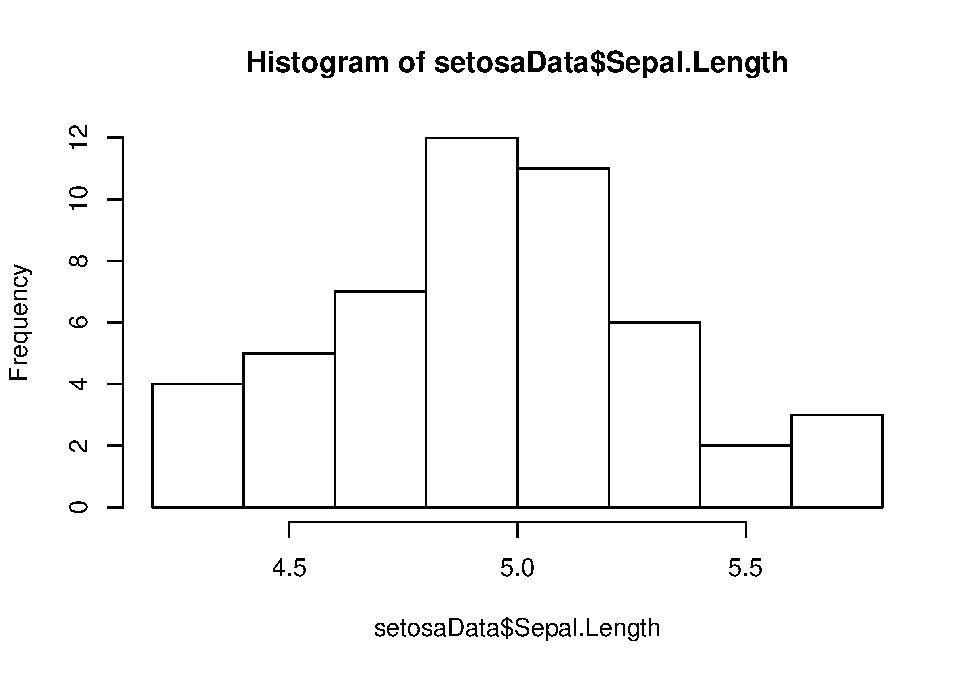
\includegraphics{worstr_files/figure-latex/unnamed-chunk-54-1.pdf}

\begin{Shaded}
\begin{Highlighting}[]
\CommentTok{# Bi-plot}
\KeywordTok{plot}\NormalTok{(setosaData}\OperatorTok{$}\NormalTok{Sepal.Width, setosaData}\OperatorTok{$}\NormalTok{Sepal.Length)}
\end{Highlighting}
\end{Shaded}

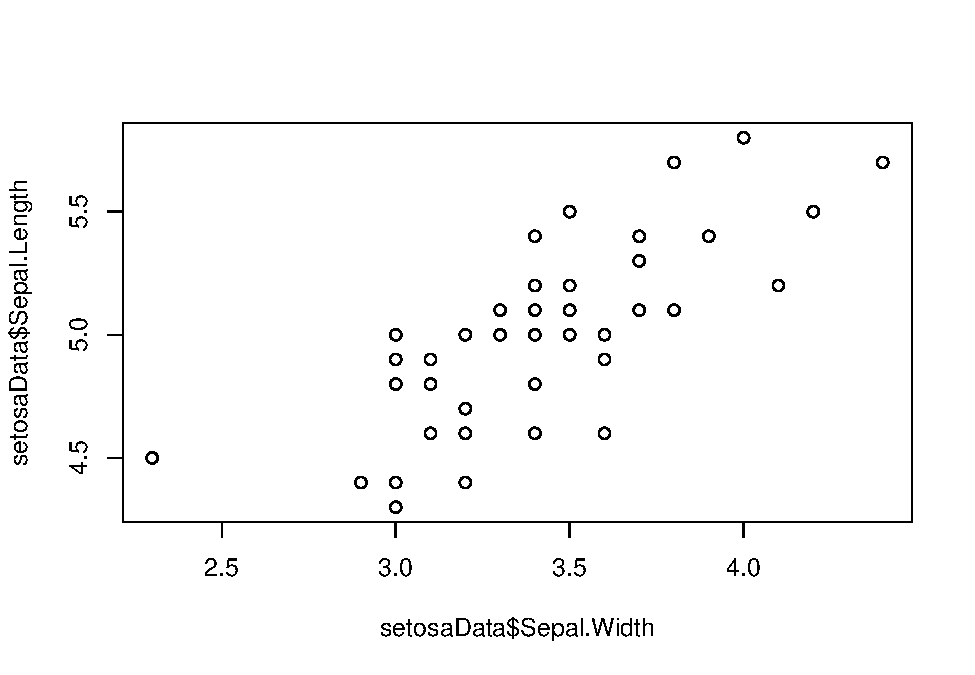
\includegraphics{worstr_files/figure-latex/unnamed-chunk-54-2.pdf}

\begin{Shaded}
\begin{Highlighting}[]
\CommentTok{# Boxplots}
\KeywordTok{boxplot}\NormalTok{(Sepal.Width }\OperatorTok{~}\StringTok{ }\NormalTok{Species, }\DataTypeTok{data =}\NormalTok{ iris)}
\end{Highlighting}
\end{Shaded}

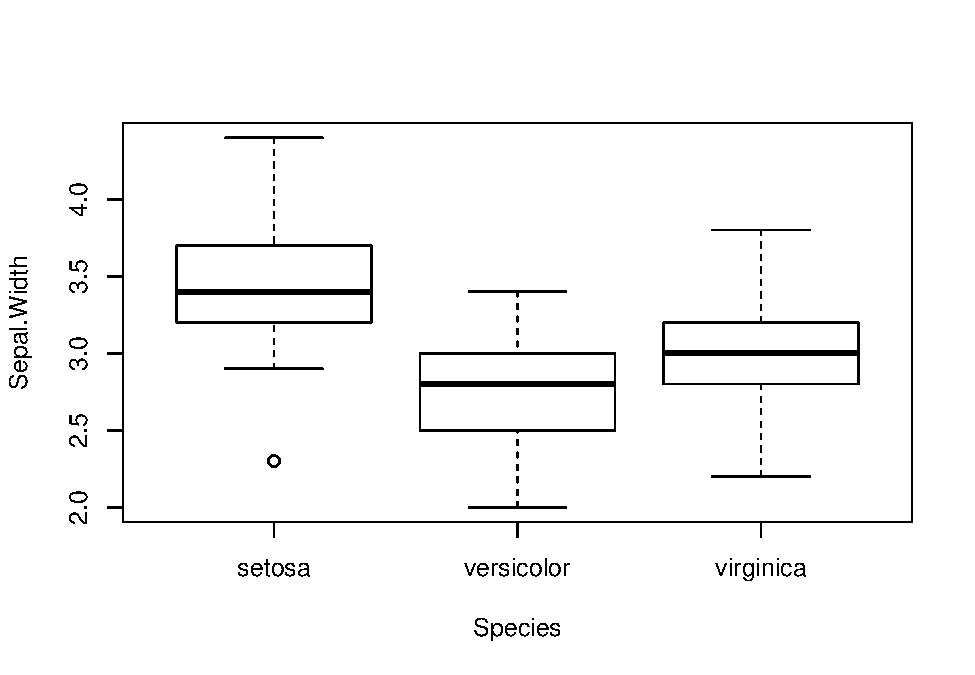
\includegraphics{worstr_files/figure-latex/unnamed-chunk-54-3.pdf}

Much, \textbf{MUCH} more of this to come as we continue.

\hypertarget{lists}{%
\section{Lists}\label{lists}}

\textbf{Lists} are the ultimate data type in R. They are actually a \href{vectors}{vector} that can hold different kinds of data, like a \protect\hyperlink{dataframes}{dataframe}. In fact, a dataframe is just a spectacularly rectangular list. Each element of a list can be any kind of object (an atomic vector, a matrix, a dataframe, or even another list!!).

Most of the real, filthy R programming relies heavily on lists. We will have to work with them at some point in this class, but we won't take a ton of time on them here.

Let's make a list- just to see how they work. Notice how our index operator has changed from \texttt{{[}\ {]}} to \texttt{{[}{[}\ {]}{]}}? And, at the highest level of organization, we have only one dimension in our list, but any given element \texttt{myList{[}{[}i{]}{]}} could hold any number of dimensions.

\begin{Shaded}
\begin{Highlighting}[]
\CommentTok{# Create an empty list with four elements}
\NormalTok{myList <-}\StringTok{ }\KeywordTok{vector}\NormalTok{(}\DataTypeTok{mode =} \StringTok{"list"}\NormalTok{, }\DataTypeTok{length =} \DecValTok{4}\NormalTok{)}

\CommentTok{# Assign some of our previously}
\CommentTok{# created objects to the elements}
\NormalTok{myList[[}\DecValTok{1}\NormalTok{]] <-}\StringTok{ }\NormalTok{a}
\NormalTok{myList[[}\DecValTok{2}\NormalTok{]] <-}\StringTok{ }\NormalTok{c}
\NormalTok{myList[[}\DecValTok{3}\NormalTok{]] <-}\StringTok{ }\NormalTok{mat}
\NormalTok{myList[[}\DecValTok{4}\NormalTok{]] <-}\StringTok{ }\NormalTok{d}
\end{Highlighting}
\end{Shaded}

Have a look at the list:

\begin{Shaded}
\begin{Highlighting}[]
\CommentTok{# Print it}
\CommentTok{# Cool, huh?}
\NormalTok{myList}
\end{Highlighting}
\end{Shaded}

\begin{verbatim}
## [[1]]
##  [1]  0.5  1.0  1.5  2.0  2.5  3.0  3.5  4.0  4.5  5.0  5.5  6.0  6.5  7.0  7.5
## [16]  8.0  8.5  9.0  9.5 10.0
## 
## [[2]]
##  [1] "a" "b" "c" "d" "a" "b" "c" "d" "a" "b" "c" "d" "a" "b" "c" "d" "a" "b" "c"
## [20] "d"
## 
## [[3]]
##        first second third
## This       1      5     9
## is         2      6    10
## a          3      7    11
## matrix     4      8    12
## 
## [[4]]
##       a      b c
## 1   0.5   0.25 a
## 2   1.0   1.00 b
## 3   1.5   2.25 c
## 4   2.0   4.00 d
## 5   2.5   6.25 a
## 6   3.0   9.00 b
## 7   3.5  12.25 c
## 8   4.0  16.00 d
## 9   4.5  20.25 a
## 10  5.0  25.00 b
## 11  5.5  30.25 c
## 12  6.0  36.00 d
## 13  6.5  42.25 a
## 14  7.0  49.00 b
## 15  7.5  56.25 c
## 16  8.0  64.00 d
## 17  8.5  72.25 a
## 18  9.0  81.00 b
## 19  9.5  90.25 c
## 20 10.0 100.00 d
\end{verbatim}

You can assign names when you create the list like we did for dataframes, too. You can do this manually, or R will do it on the fly for you. You can also reassign names to a list that yo've already created.

\begin{Shaded}
\begin{Highlighting}[]
\CommentTok{# No names by default}
\KeywordTok{names}\NormalTok{(myList)}

\CommentTok{# Give it names like we did with}
\CommentTok{# a dataframe}
\KeywordTok{names}\NormalTok{(myList) <-}\StringTok{ }\KeywordTok{c}\NormalTok{(}\StringTok{"a"}\NormalTok{, }\StringTok{"c"}\NormalTok{, }\StringTok{"mat"}\NormalTok{, }\StringTok{"d"}\NormalTok{)}

\CommentTok{# See how the names work now?}
\NormalTok{myList}

\CommentTok{# We reference these differently [[]]}
\NormalTok{myList[[}\DecValTok{1}\NormalTok{]]}

\CommentTok{# But we can still get into each object}
\CommentTok{# Play around with the numbers to see what they do!}
\NormalTok{myList[[}\DecValTok{2}\NormalTok{]][}\DecValTok{5}\NormalTok{]}

\CommentTok{# Can also reference it this way!}
\NormalTok{myList}\OperatorTok{$}\NormalTok{c[}\DecValTok{1}\NormalTok{]}
\end{Highlighting}
\end{Shaded}

Very commonly, model objects and output are stored as lists. In fact, most objects that require a large amount of diverse information in R pack it all together in one place using lists, that way we always know where to find it and how as long as the objects are documented. Conceptually, every object in R, from your workspace on down the line, is a list \textbf{AND} an element of a list. It seems like a lot to take in now, but will be very useful in the future.

\hypertarget{next2}{%
\section{Next steps}\label{next2}}

For more practice with the data structures and R functions we covered here, you can check out this walk-through of basic R commands from the How To R YouTube Channel.

In the Chapter 3(\#Chapter3), we will begin using functions from external R packages to read and work with real data.

\hypertarget{Chapter3}{%
\chapter{Working with data}\label{Chapter3}}

American shad, the best fish, lost in the data deluge. Let's figure out how to make some sense of it.

The purpose of this chapter is to get you comfortable working with data in R and give you some tools for summarizing those data in a meaningful way. This is not meant to be a comprehensive treatment of these subjects but rather an introduction to the tools that are available to you (say it with me: ``Worst Stats Text eveR''). There are a lot of tools out there and you may come up with something that works better for you once you have some basics under your belt.

Now that you have a handle on the types of data you can expect to run into in R, let's have a look at how we read and work with data that we get from the real world.

We will work with the \texttt{ctr\_fish.csv} file for Chapter 3, so you will need to download the class data sets that go with this book to play along. We will also need the \texttt{tidyverse} package, but instructions for installation are provided below because this is the first time we have downloaded and installed a package.

\hypertarget{data-read}{%
\section{Data read}\label{data-read}}

There are few things that will turn someone away from a statistical software program faster than if they can't even figure out how to get the program to read in their data. So, we are going to get it out of the way right up front!

Let's start by reading in a data file - this time we use real data.

The data are stored in a ``comma separated values'' file (\texttt{.csv} extension). This is a fairly universal format, so we read it in using the fairly universal \texttt{read.csv()} function. This would change depending on how the data were stored, or how big the data files were, but that is a topic further investigation for a later date. I probably do 95\% of my data reads using \texttt{.csv} files. We'll look at a few others later.

\textbf{Important} Remember that I am assuming your scripts are in the same directory (folder) on your computer as where you downloaded and unzipped the class data (see \href{https://danstich.github.io/stich/classes/BIOL217/software.html}{here} for reminder).

\textbf{Before you can read this file} you will need to set your working directory. For class, I will ask that you click \texttt{Session\ \textgreater{}\ Set\ Working\ Directory\ \textgreater{}\ To\ Source\ File\ Location}. This will set the working directory to wherever you have saved your code so that R can find the folder \texttt{data} and the files inside of it. You'll notice that R spits out some code in the console when you click this. You can also use that code to set a working directory in your script but that can cause \href{https://support.rstudio.com/hc/en-us/articles/200711843-Working-Directories-and-Workspaces}{all kinds of problems}, so don't do it.

\begin{Shaded}
\begin{Highlighting}[]
\CommentTok{# Start by reading in the data}
\NormalTok{am_shad <-}\StringTok{ }\KeywordTok{read.csv}\NormalTok{(}\StringTok{"data/ctr_fish.csv"}\NormalTok{)}
\end{Highlighting}
\end{Shaded}

Once you've read your data in, it's always a good idea to look at the first few lines of data to make sure nothing looks `fishy'. Ha-ha, I couldn't help myself!

These are sex-specific length and age data for American shad (\emph{Alosa sapidissima}) from the Connecticut River, USA. The data are used in models that I maintain with collaborators from NOAA Fisheries, the US Geological Survey, the US Fish and Wildlife Service, and others. The data were provided by CT Department of Energy and Environmental Protection (CTDEEP) and come from adult fish that return to the river from the ocean each year to spawn in fresh water.

You can look at the first few rows of data with the \texttt{head()} function:

\begin{Shaded}
\begin{Highlighting}[]
\CommentTok{# Look at the first 10 rows}
\KeywordTok{head}\NormalTok{(am_shad, }\DecValTok{10}\NormalTok{)}
\end{Highlighting}
\end{Shaded}

\begin{verbatim}
##    Sex Age Length yearCollected backCalculated Mass
## 1    B   1     13          2010           TRUE   NA
## 2    B   1     15          2010           TRUE   NA
## 3    B   1     15          2010           TRUE   NA
## 4    B   1     15          2010           TRUE   NA
## 5    B   1     15          2010           TRUE   NA
## 6    B   1     15          2010           TRUE   NA
## 7    B   1     16          2010           TRUE   NA
## 8    B   1     16          2010           TRUE   NA
## 9    B   1     16          2010           TRUE   NA
## 10   B   1     16          2010           TRUE   NA
\end{verbatim}

The \texttt{NA} values are supposed to be there. They are missing data.

And, don't forget about your old friend \texttt{str()} for a peek at how R sees your data. This can take care of a lot of potential problems later on.

\begin{Shaded}
\begin{Highlighting}[]
\CommentTok{# Look at the structure of the data}
\KeywordTok{str}\NormalTok{(am_shad)}
\end{Highlighting}
\end{Shaded}

\begin{verbatim}
## 'data.frame':	16946 obs. of  6 variables:
##  $ Sex           : Factor w/ 2 levels "B","R": 1 1 1 1 1 1 1 1 1 1 ...
##  $ Age           : int  1 1 1 1 1 1 1 1 1 1 ...
##  $ Length        : num  13 15 15 15 15 15 16 16 16 16 ...
##  $ yearCollected : int  2010 2010 2010 2010 2010 2010 2010 2010 2010 2010 ...
##  $ backCalculated: logi  TRUE TRUE TRUE TRUE TRUE TRUE ...
##  $ Mass          : int  NA NA NA NA NA NA NA NA NA NA ...
\end{verbatim}

There are about 17,000 observations (rows) of 6 variables (columns) in this data set. Here is a quick breakdown:

\texttt{Sex}: fish gender. \texttt{B} stands for `buck' (males), \texttt{R} stands for `roe' (females).\\

\texttt{Age}: an integer describing fish age.\\

\texttt{Length}: fish length at age (cm).\\

\texttt{yearCollected}: the year in which the fish was caught.\\

\texttt{backCalculated}: a logical indicating whether or not the length
of the fish was back-calculated from aging.\\

\texttt{Mass}: the mass of indnividual fish (in grams). Note that this is NA
for all ages that were estimated from hard structures (so all
cases for which \texttt{backCalculated\ ==\ TRUE}).

\hypertarget{quick-data-summaries}{%
\section{Quick data summaries}\label{quick-data-summaries}}

There are a number of simple ways to summarize data quickly in base R. We already looked at a few of these in previous chapters. But what about something a little more in-depth?

One quick way to look at your data is using the \texttt{summary()} function

\begin{Shaded}
\begin{Highlighting}[]
\KeywordTok{summary}\NormalTok{(am_shad)}
\end{Highlighting}
\end{Shaded}

\begin{verbatim}
##  Sex           Age            Length      yearCollected  backCalculated 
##  B:9512   Min.   :1.000   Min.   : 3.00   Min.   :2010   Mode :logical  
##  R:7434   1st Qu.:2.000   1st Qu.:31.00   1st Qu.:2011   FALSE:3046     
##           Median :3.000   Median :38.00   Median :2012   TRUE :13900    
##           Mean   :3.155   Mean   :36.39   Mean   :2012                  
##           3rd Qu.:4.000   3rd Qu.:43.00   3rd Qu.:2013                  
##           Max.   :7.000   Max.   :55.00   Max.   :2014                  
##                                                                         
##       Mass      
##  Min.   :   0   
##  1st Qu.: 900   
##  Median :1120   
##  Mean   :1173   
##  3rd Qu.:1440   
##  Max.   :3280   
##  NA's   :14115
\end{verbatim}

This is useful for getting the big-picture. For continuous variables (e.g., \texttt{Age} and \texttt{Length}) R will report some descriptive statistics like the \texttt{mean}, \texttt{median}, and quantiles. For discrete variables (e.g.~\texttt{Sex} and \texttt{backCalculated}) we get the mode (if not \texttt{factor} or \texttt{chr}) and counts of observations within each discrete level (e.g.~number of observations of \texttt{B} and \texttt{R} in the variable \texttt{Sex}).

But, this approach doesn't really give us much info.

We can create more meaningful summaries pretty easily if we install and load some packages like we talked about in \protect\hyperlink{Chapter1}{Chapter 1}, and then look at different ways of sub-setting the data with base R and some methods that might be a little more intuitive for you.

\hypertarget{subsetting-and-selecting-data}{%
\section{Subsetting and selecting data}\label{subsetting-and-selecting-data}}

Before we can make meaningful data summaries, we will probably need to re-organize our data in a logical way (through sub-setting or selected specific chunks of data). A lot of times, we do this along the way without really thinking about it.

\hypertarget{manual-subsets-and-selections}{%
\subsection{Manual subsets and selections}\label{manual-subsets-and-selections}}

We talked a little about sub-setting data with logical queries in \protect\hyperlink{Chapter2}{Chapter 2}. Now, let's refresh and take that a little further to see why we might want to do that.

First, we'll select just the data from \texttt{am\_shad} where \texttt{backCalculated} was \texttt{FALSE}. This will give us only the measured \texttt{Length} and \texttt{Mass} for each of the fish, along with their \texttt{Sex} and \texttt{yearCollected}. I'll call this new object \texttt{measured}. Remember, \texttt{am\_shad} is a data frame, so it has two dimensions when we use \texttt{{[}\ {]}} for sub-setting and these are separated by a comma, like this: \texttt{object{[}rows,\ columns{]}}. When we leave the columns blank, R knows that it should keep all of the columns.

\begin{Shaded}
\begin{Highlighting}[]
\NormalTok{measured <-}\StringTok{ }\NormalTok{am_shad[am_shad}\OperatorTok{$}\NormalTok{backCalculated }\OperatorTok{==}\StringTok{ }\OtherTok{FALSE}\NormalTok{, ]}
\end{Highlighting}
\end{Shaded}

We could do this for as many conceivable conditions in our data on which we may wish to subset, but the code can get clunky and hard to manage. For example can you imagine re-writing this if you just want to select age six roes without back-calculated lengths?

\begin{Shaded}
\begin{Highlighting}[]
\CommentTok{# Notice how we string together multiple }
\CommentTok{# conditions with "&". If these were 'or'}
\CommentTok{# we would use the vertical pipe "|"}
\NormalTok{age_}\DecValTok{6}\NormalTok{_rows_measured <-}\StringTok{ }\NormalTok{am_shad[am_shad}\OperatorTok{$}\NormalTok{backCalculated }\OperatorTok{==}\StringTok{ }\OtherTok{FALSE} \OperatorTok{&}\StringTok{ }
\StringTok{                                 }\NormalTok{am_shad}\OperatorTok{$}\NormalTok{Sex }\OperatorTok{==}\StringTok{ "R"} \OperatorTok{&}
\StringTok{                                 }\NormalTok{am_shad}\OperatorTok{$}\NormalTok{Age }\OperatorTok{==}\StringTok{ }\DecValTok{6}\NormalTok{, ]}
\end{Highlighting}
\end{Shaded}

\hypertarget{subsetting-and-summaries-in-base-r}{%
\subsection{Subsetting and summaries in base R}\label{subsetting-and-summaries-in-base-r}}

This notation can be really confusing to folks who are just trying to learn a new programming language. Because of that, there are great functions like \texttt{subset()} available that are more intuitive (but less clear to programmers). You could also subset the data using the following code:

\begin{Shaded}
\begin{Highlighting}[]
\NormalTok{measured <-}\StringTok{ }\KeywordTok{subset}\NormalTok{(am_shad, backCalculated }\OperatorTok{==}\StringTok{ }\OtherTok{FALSE}\NormalTok{)}
\end{Highlighting}
\end{Shaded}

We could also get our age-six females from the previous example using this approach, and at least the code is a little cleaner:

\begin{Shaded}
\begin{Highlighting}[]
\NormalTok{age_}\DecValTok{6}\NormalTok{_roes_measured <-}\StringTok{ }\KeywordTok{subset}\NormalTok{(am_shad,}
\NormalTok{                              backCalculated }\OperatorTok{==}\StringTok{ }\OtherTok{FALSE} \OperatorTok{&}
\StringTok{                                }\NormalTok{Sex }\OperatorTok{==}\StringTok{ "R"} \OperatorTok{&}
\StringTok{                                }\NormalTok{Age }\OperatorTok{==}\StringTok{ }\DecValTok{6}
\NormalTok{                              )}
\end{Highlighting}
\end{Shaded}

Both do the same thing, but we'll see later that using \texttt{subset} is preferable if we plan on chaining together a bunch of data manipulation commands using pipes (\texttt{\%\textgreater{}\%}).

Next, we might be interested to know how many fish we have represented in each \texttt{Sex}. We can find this out using the \texttt{table} function in base R:

\begin{Shaded}
\begin{Highlighting}[]
\CommentTok{# Here, I use the column name because}
\CommentTok{# we just want all observations of a single}
\CommentTok{# variable. Be careful switching between names,}
\CommentTok{# numbers, and $names!}
\KeywordTok{table}\NormalTok{(measured[}\StringTok{'Sex'}\NormalTok{])}
\end{Highlighting}
\end{Shaded}

\begin{verbatim}
## 
##    B    R 
## 1793 1253
\end{verbatim}

We see that we have \texttt{1793} females and \texttt{1253} males.

We can also get tallies of the number of fish in each \texttt{Age} for each \texttt{Sex} if we would like to see that:

\begin{Shaded}
\begin{Highlighting}[]
\KeywordTok{table}\NormalTok{(measured}\OperatorTok{$}\NormalTok{Sex, measured}\OperatorTok{$}\NormalTok{Age)}
\end{Highlighting}
\end{Shaded}

\begin{verbatim}
##    
##       3   4   5   6   7
##   B 255 848 579 108   3
##   R   0 361 658 220  14
\end{verbatim}

But, what if we wanted to calculate some kind of summary statistic, like a \texttt{mean} and report that by group?

For our age-6 females example, it would look like this:

\begin{Shaded}
\begin{Highlighting}[]
\NormalTok{age_}\DecValTok{6}\NormalTok{_roes_measured <-}\StringTok{ }\KeywordTok{subset}\NormalTok{(am_shad,}
\NormalTok{                              backCalculated }\OperatorTok{==}\StringTok{ }\OtherTok{FALSE} \OperatorTok{&}
\StringTok{                                }\NormalTok{Sex }\OperatorTok{==}\StringTok{ "R"} \OperatorTok{&}
\StringTok{                                }\NormalTok{Age }\OperatorTok{==}\StringTok{ }\DecValTok{6}
\NormalTok{                              )}

\NormalTok{age_}\DecValTok{6}\NormalTok{_female_mean <-}\StringTok{ }\KeywordTok{mean}\NormalTok{(age_}\DecValTok{6}\NormalTok{_roes_measured}\OperatorTok{$}\NormalTok{Length)}
\end{Highlighting}
\end{Shaded}

Again, we could do this manually, but would require a lot of code for a simple calculation if we use the methods above all by themselves to get these for each age group of roes.

We would basically just copy-and-paste the code over and over to force R into making the data summaries we need. Nothing wrong with this approach, and it certainly has its uses for simple summaries, but it can be cumbersome and redundant. It also fills your workspace up with tons of objects that are hard to keep track of and that will cause your code-completion suggestions to be \emph{wicked} annoying in RStudio.

That usually means there is a better way to write the code\ldots{}

\hypertarget{tidyverse}{%
\subsection{Subsetting and summaries in the tidyverse}\label{tidyverse}}

Long ago, when I was still a noOb writing R code with a stand-alone text editor and a console there were not a ton of packages available for the express purpose of cleaning up data manipulation in R. The one I relied on most heavily was the \texttt{plyr} package. Since then, R has grown and a lot of these functions have been gathered under the umbrella of the \href{https://www.tidyverse.org/packages/}{tidyverse}, which is a collection of specific R packages designed to make the whole process less painful. These include packages like \texttt{dplyr} (which replaced \texttt{plyr}) and others that are designed to work together with similar syntax to make data science (for us, data manipulation and presentation) a lot cleaner and better standardized. We will rely heavily on packages in the tidyverse throughout this book.

Before we can work with these packages, however, we need to install them - something we haven't talked about yet! Most of the critical R packages are hosted through the Comprehensive R Archive Network, or \href{https://cran.r-project.org/}{CRAN}. Still, tons of others are available for installation from hosting services like GitHub and GitLab.

If you haven't seen it yet, \href{https://www.youtube.com/watch?v=u1r5XTqrCTQ}{here} is a three-minute video explaining how to install packages using RStudio. \textbf{Watch it. Please.}

It is also easy to install packages by running a line of code in the console. We could install each of the packages in the tidyverse separately. But we can also get all of them at once because they are all packaged together, too.

Follow the instructions in the YouTube link above, or install the package from the command line:

\begin{Shaded}
\begin{Highlighting}[]
\KeywordTok{install.packages}\NormalTok{(}\StringTok{'tidyverse'}\NormalTok{)}
\end{Highlighting}
\end{Shaded}

Once we have installed these packages, we can use the functions in them to clean up our data manipulation pipeline and get some really useful information.

\hypertarget{better-data-summaries}{%
\section{Better data summaries}\label{better-data-summaries}}

Now, we'll look at some slightly more advanced summaries. Start by loading the \texttt{dplyr} package into your R session with the following code.

\begin{Shaded}
\begin{Highlighting}[]
\KeywordTok{library}\NormalTok{(dplyr)}
\end{Highlighting}
\end{Shaded}

We can use functions from the \texttt{dplyr} package to calculate mean \texttt{Length} of fish for each combination of \texttt{Sex} and \texttt{Age} group much more easily than we did for a single group above.

First, we group the data in \texttt{measured} data frame that we created previously using the \texttt{group\_by} function. For this, we just need to give R the data frame and the variables by which we would like to group:

\begin{Shaded}
\begin{Highlighting}[]
\NormalTok{g_lengths <-}\StringTok{ }\KeywordTok{group_by}\NormalTok{(measured, Sex, Age)}
\end{Highlighting}
\end{Shaded}

This doesn't change how we see the data much (it gets converted to a \href{https://tibble.tidyverse.org/\#:~:text=A\%20tibble\%2C\%20or\%20tbl_df\%20\%2C\%20is,modern\%20reimagining\%20of\%20the\%20data.\&text=Tibbles\%20are\%20data.,a\%20variable\%20does\%20not\%20exist}{\texttt{tibble}}), just how R sees it.

Next, we summarize the variable \texttt{Length} by \texttt{Sex} and \texttt{Age} using the \texttt{summarize} function:

\begin{Shaded}
\begin{Highlighting}[]
\NormalTok{sum_out <-}\StringTok{ }\KeywordTok{summarize}\NormalTok{(g_lengths, }\DataTypeTok{avg =} \KeywordTok{mean}\NormalTok{(Length))}

\KeywordTok{head}\NormalTok{(sum_out)}
\end{Highlighting}
\end{Shaded}

\begin{verbatim}
## # A tibble: 6 x 3
## # Groups:   Sex [2]
##   Sex     Age   avg
##   <fct> <int> <dbl>
## 1 B         3  38.1
## 2 B         4  40.5
## 3 B         5  42.0
## 4 B         6  43.4
## 5 B         7  46.8
## 6 R         4  45.0
\end{verbatim}

Wow! That was super-easy!

Finally, to make things even more streamlined, we can chain all of these operations together using the \texttt{\%\textgreater{}\%} function from \texttt{magrittr}. This really cleans up the code and gives us small chunks of code that are easier to read than the dozens of lines of code it would take to do this manually.

\begin{Shaded}
\begin{Highlighting}[]
\CommentTok{# This will do it all at once!}
\NormalTok{sum_out <-}\StringTok{ }\CommentTok{# Front-end object assignment}
\StringTok{  }\NormalTok{measured }\OperatorTok\StringTok{ }\CommentTok{# Pass measured to the group_by function}
\StringTok{  }\KeywordTok{group_by}\NormalTok{(Sex, Age) }\OperatorTok\StringTok{ }\CommentTok{# Group by Sex and age and pass to summarize}
\StringTok{  }\KeywordTok{summarize}\NormalTok{(}\DataTypeTok{avg =} \KeywordTok{mean}\NormalTok{(Length))}
\end{Highlighting}
\end{Shaded}

We could also assign the output to a variable at the end, whichever is easier for you to read:

\begin{Shaded}
\begin{Highlighting}[]
\NormalTok{  measured }\OperatorTok\StringTok{ }\CommentTok{# Pass measured to the group_by function}
\StringTok{  }\KeywordTok{group_by}\NormalTok{(Sex, Age) }\OperatorTok\StringTok{ }\CommentTok{# Group by Sex and age and pass to summarize}
\StringTok{  }\KeywordTok{summarize}\NormalTok{(}\DataTypeTok{avg =} \KeywordTok{mean}\NormalTok{(Length)) ->}\StringTok{ }\NormalTok{sim_out }\CommentTok{# Back-end object assignment}
\end{Highlighting}
\end{Shaded}

And, it is really easy to get multiple summaries out like this at once:

\begin{Shaded}
\begin{Highlighting}[]
\NormalTok{sum_out <-}
\StringTok{  }\NormalTok{measured }\OperatorTok\StringTok{ }
\StringTok{  }\KeywordTok{group_by}\NormalTok{(Sex, Age) }\OperatorTok\StringTok{ }
\StringTok{  }\KeywordTok{summarize}\NormalTok{(}\DataTypeTok{avg =} \KeywordTok{mean}\NormalTok{(Length), }\DataTypeTok{s.d. =} \KeywordTok{sd}\NormalTok{(Length))}

\KeywordTok{head}\NormalTok{(sum_out)}
\end{Highlighting}
\end{Shaded}

\begin{verbatim}
## # A tibble: 6 x 4
## # Groups:   Sex [2]
##   Sex     Age   avg  s.d.
##   <fct> <int> <dbl> <dbl>
## 1 B         3  38.1  2.75
## 2 B         4  40.5  2.70
## 3 B         5  42.0  2.29
## 4 B         6  43.4  2.09
## 5 B         7  46.8  1.61
## 6 R         4  45.0  2.65
\end{verbatim}

Isn't that slick? Just think how long that would have taken most of us in Excel!

This is just one example of how functions in packages can make your life easier and your code more efficient. Now that we have the basics under our belts, lets move on to how we create new variables.

\hypertarget{creating-new-variables}{%
\section{Creating new variables}\label{creating-new-variables}}

There are basically two ways to create new variables: we can modify an existing variable (groups or formulas), or we can simulate new values for that variable (random sampling.)

If we have a formula that relates two variables, we could predict one based on the other deterministically.

For example, I have fit a length-weight regression to explain the relationship between \texttt{Length} and \texttt{Mass} using the \texttt{am\_shad} data we've worked with in previous sections.

This relationship looks like your old friend \(y = mx + b\), the equation for a line, but we log10-transform both of the variables before fitting the line (more to come later in the class). Using this relationship, we can predict our \textbf{independent variable} (\texttt{Mass}) from our \textbf{dependent variable} (\texttt{Length}) if we plug in new values for \texttt{Length} and the \textbf{parameters} of the line.

In this case, I know that \texttt{m} = 3.0703621, and \texttt{b} = -1.9535405.

If I plug these numbers in to the equation above, I can predict \texttt{log10(Mass)} for new lengths \texttt{log10(Length)}:

\(log_{10}Mass = 3.0703621 \cdot log_{10}Length - 1.9535405\)

In R, this looks like:

\begin{Shaded}
\begin{Highlighting}[]
\CommentTok{# Parameters from length-weight regression}
\NormalTok{m <-}\StringTok{ }\FloatTok{3.0703621}
\NormalTok{b <-}\StringTok{ }\FloatTok{1.9535405}

\CommentTok{# Make a sequence of new lengths based on range in data,}
\CommentTok{# then take the log of the whole thing all at once.}
\NormalTok{log_length <-}\StringTok{ }\KeywordTok{log10}\NormalTok{( }\KeywordTok{seq}\NormalTok{(}\KeywordTok{min}\NormalTok{(am_shad}\OperatorTok{$}\NormalTok{Length), }\KeywordTok{max}\NormalTok{(am_shad}\OperatorTok{$}\NormalTok{Length), }\DecValTok{1}\NormalTok{) )}

\CommentTok{# Calculate a new thing (log10_mass) using parameters for line}
\CommentTok{# and sequence of new log10_length.}
\NormalTok{log_mass <-}\StringTok{ }\NormalTok{m }\OperatorTok{*}\StringTok{ }\NormalTok{log_length }\OperatorTok{+}\StringTok{ }\NormalTok{b}

\CommentTok{# Plot the prediction}
\KeywordTok{plot}\NormalTok{(}\DataTypeTok{x =}\NormalTok{ log_length, }\DataTypeTok{y =}\NormalTok{ log_mass, }\DataTypeTok{type =} \StringTok{"l"}\NormalTok{)}
\end{Highlighting}
\end{Shaded}

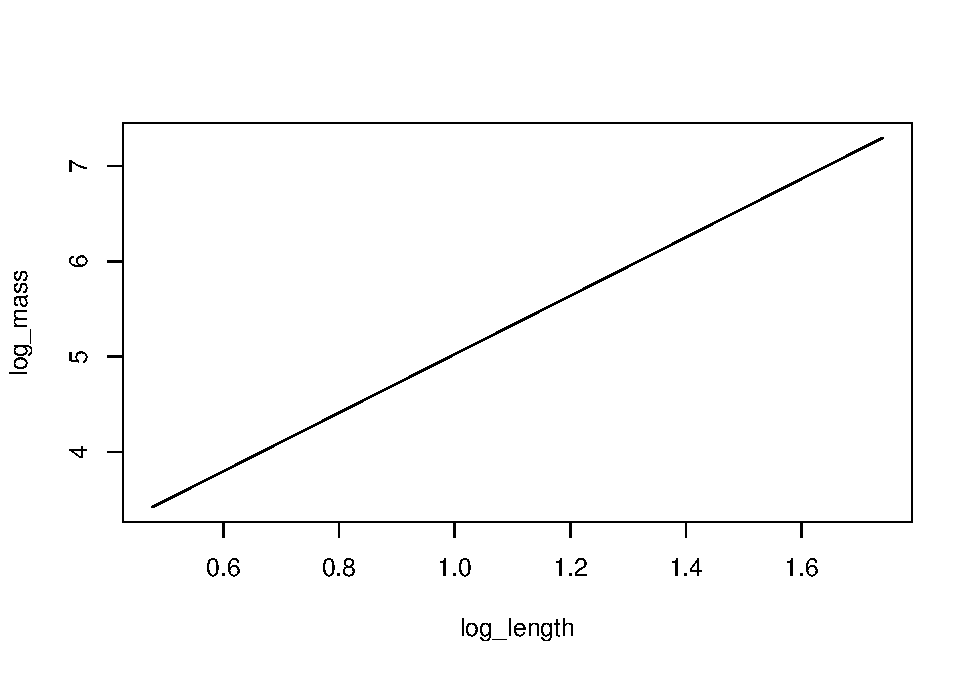
\includegraphics{worstr_files/figure-latex/unnamed-chunk-77-1.pdf}

\hypertarget{data-simulation}{%
\section{Data simulation}\label{data-simulation}}

The point of simulation is usually to account for uncertainty in some process (i.e.~we could just pick a single value if we knew it). This is almost always done based on probability. There are a number of ways we could do this. One is by drawing from some probability distribution that we have described, and the other is by randomly sampling data that we already have.

\hypertarget{random-sub-samples-from-a-dataset}{%
\subsection{Random sub-samples from a dataset}\label{random-sub-samples-from-a-dataset}}

Let's say we want to take random samples from our huge data set so we can fit models to a subset of data and then use the rest of our data for model validation in weeks to come.

We have around 17,000 observations in the \texttt{am\_shad} data set. But, what if we wanted to know what it would look like if we only had 100 samples from the same population?

First, tell R how many samples you want.

\begin{Shaded}
\begin{Highlighting}[]
\NormalTok{n_samples <-}\StringTok{ }\DecValTok{100}
\end{Highlighting}
\end{Shaded}

Now let's take two samples of 100 fish from our dataframe to see how they compare:

\begin{Shaded}
\begin{Highlighting}[]
\CommentTok{# Randomly sample 100 rows of data from our data frame two different}
\CommentTok{# times to see the differences}
\NormalTok{samp1 <-}\StringTok{ }\NormalTok{am_shad[}\KeywordTok{sample}\NormalTok{(}\KeywordTok{nrow}\NormalTok{(am_shad), }\DataTypeTok{size =}\NormalTok{ n_samples, }\DataTypeTok{replace =} \OtherTok{FALSE}\NormalTok{), ]}
\NormalTok{samp2 <-}\StringTok{ }\NormalTok{am_shad[}\KeywordTok{sample}\NormalTok{(}\KeywordTok{nrow}\NormalTok{(am_shad), }\DataTypeTok{size =}\NormalTok{ n_samples, }\DataTypeTok{replace =} \OtherTok{FALSE}\NormalTok{), ]}

\CommentTok{# We can look at them with our histograms}
\KeywordTok{par}\NormalTok{(}\DataTypeTok{mfrow =} \KeywordTok{c}\NormalTok{(}\DecValTok{1}\NormalTok{, }\DecValTok{2}\NormalTok{))}
\KeywordTok{hist}\NormalTok{(samp1}\OperatorTok{$}\NormalTok{Length, }\DataTypeTok{main =} \StringTok{""}\NormalTok{, }\DataTypeTok{ylim =} \KeywordTok{c}\NormalTok{(}\DecValTok{0}\NormalTok{, }\DecValTok{30}\NormalTok{))}
\KeywordTok{hist}\NormalTok{(samp2}\OperatorTok{$}\NormalTok{Length, }\DataTypeTok{main =} \StringTok{""}\NormalTok{, }\DataTypeTok{ylim =} \KeywordTok{c}\NormalTok{(}\DecValTok{0}\NormalTok{, }\DecValTok{30}\NormalTok{))}
\end{Highlighting}
\end{Shaded}

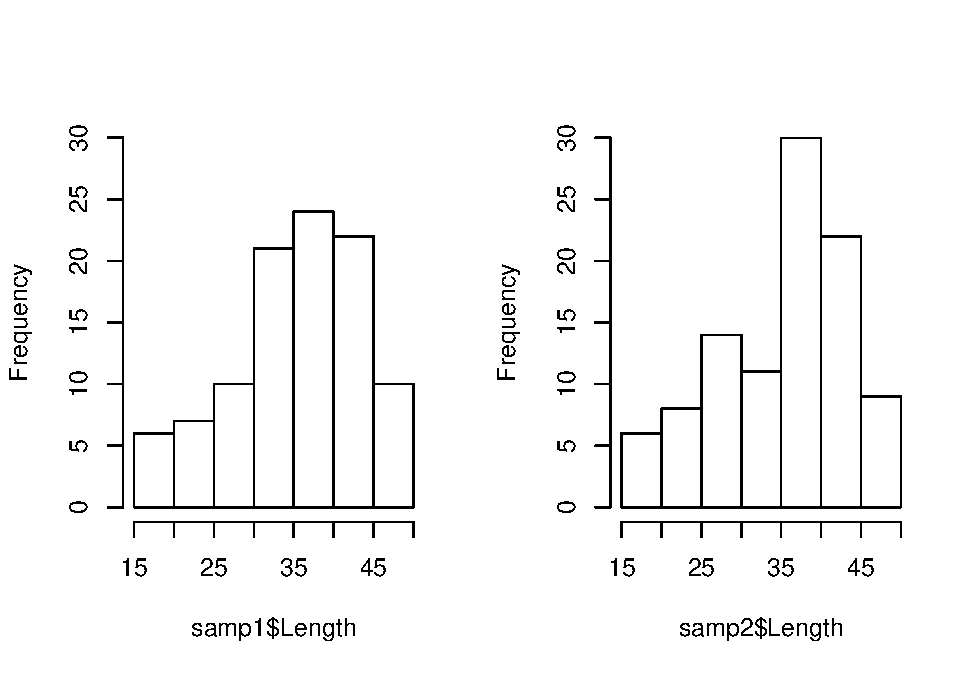
\includegraphics{worstr_files/figure-latex/unnamed-chunk-79-1.pdf}
*If you are struggling to get your plotting window back to ``normal'' after this, you can either click the broom button in your ``Plots'' window, or you can run the following code for now:

\hypertarget{stochastic}{%
\subsection{Stochastic simulation}\label{stochastic}}

Now, instead of sampling our data let's say we have some distribution from which we would like sample. So, let's make a distribution.

We will start with the normal, and we can move into others when we talk about probability distributions and sample statistics in \protect\hyperlink{Chapter5}{Chapter 5}. For this, we will use the distribution of American shad lengths for age-6 females because it approximates a normal distribution. We will calculate the \texttt{mean} and \texttt{sd} because those are the parameters of the normal distribution.

Start by looking at the size distribution for age 6 females. We use the tidy workflow here with really awful default graphics (more to come in \protect\hyperlink{Chapter4}{Chapter 4}), but we add two arguments to our \texttt{subset} call. We want to select only the variable \texttt{Length} from \texttt{am\_shad}, and we want to drop all other information so we can send the output straight to the \texttt{hist()} function as a vector.

\begin{Shaded}
\begin{Highlighting}[]
\NormalTok{am_shad }\OperatorTok
\StringTok{  }\KeywordTok{subset}\NormalTok{(Age }\OperatorTok{==}\StringTok{ }\DecValTok{6} \OperatorTok{&}\StringTok{ }\NormalTok{Sex }\OperatorTok{==}\StringTok{ "R"}\NormalTok{, }\DataTypeTok{select=}\StringTok{'Length'}\NormalTok{, }\DataTypeTok{drop=}\OtherTok{TRUE}\NormalTok{) }\OperatorTok
\StringTok{   }\KeywordTok{hist}\NormalTok{(}\DataTypeTok{main =} \StringTok{""}\NormalTok{)}
\end{Highlighting}
\end{Shaded}

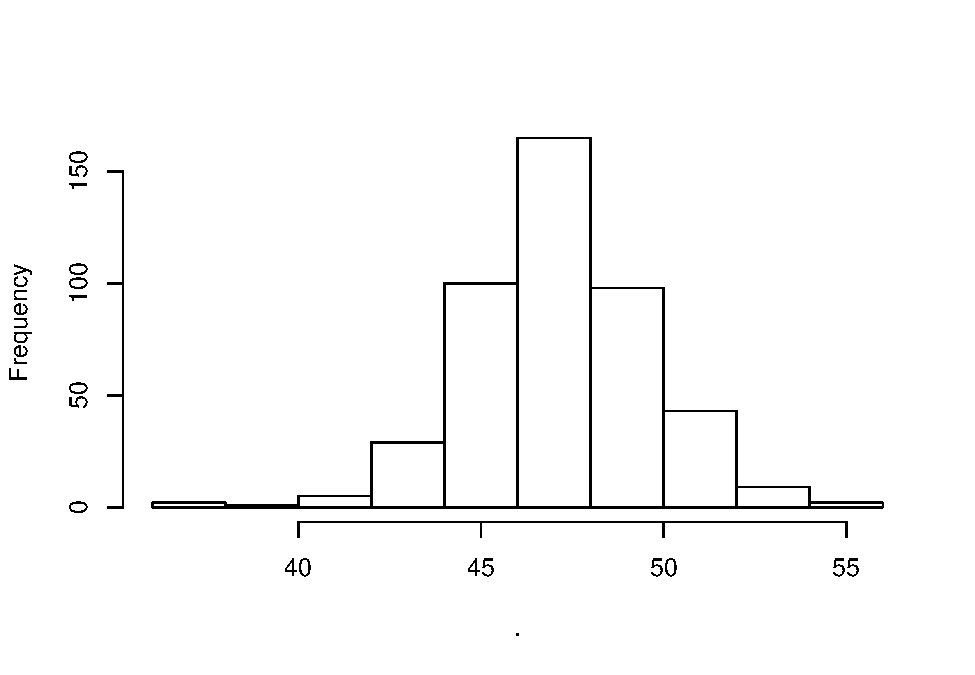
\includegraphics{worstr_files/figure-latex/unnamed-chunk-81-1.pdf}

Now, let's calculate the \texttt{mean} and \texttt{sd} of \texttt{Length} for age 6 females.

\begin{Shaded}
\begin{Highlighting}[]
\CommentTok{# Calculate the mean Length }
\NormalTok{x_bar <-}\StringTok{ }\NormalTok{am_shad }\OperatorTok
\StringTok{  }\KeywordTok{subset}\NormalTok{(Age }\OperatorTok{==}\StringTok{ }\DecValTok{6} \OperatorTok{&}\StringTok{ }\NormalTok{Sex }\OperatorTok{==}\StringTok{ "R"}\NormalTok{, }\DataTypeTok{select=}\StringTok{'Length'}\NormalTok{, }\DataTypeTok{drop=}\OtherTok{TRUE}\NormalTok{) }\OperatorTok
\StringTok{  }\NormalTok{mean}

\CommentTok{# Calculate standard deviation of Length}
\NormalTok{sigma <-}\StringTok{ }\NormalTok{am_shad }\OperatorTok
\StringTok{  }\KeywordTok{subset}\NormalTok{(Age }\OperatorTok{==}\StringTok{ }\DecValTok{6} \OperatorTok{&}\StringTok{ }\NormalTok{Sex }\OperatorTok{==}\StringTok{ "R"}\NormalTok{, }\DataTypeTok{select=}\StringTok{'Length'}\NormalTok{, }\DataTypeTok{drop=}\OtherTok{TRUE}\NormalTok{) }\OperatorTok
\StringTok{  }\NormalTok{sd}
\end{Highlighting}
\end{Shaded}

Note that we could also use the \texttt{filter()} function from the \texttt{dplyr} package for this job, and for big data sets it would be a lot faster for un-grouped data.

Now, we can use the mean and standard deviation to randomly sample our normal distribution of lengths.

\begin{Shaded}
\begin{Highlighting}[]
\CommentTok{# Take a random sample from a normal distribution}
\NormalTok{length_sample <-}\StringTok{ }\KeywordTok{rnorm}\NormalTok{(}\DataTypeTok{n =} \DecValTok{10000}\NormalTok{, }\DataTypeTok{mean =}\NormalTok{ x_bar, }\DataTypeTok{sd =}\NormalTok{ sigma)}

\CommentTok{# Plot the sample to see if it is a normal- YAY it is!}
\KeywordTok{hist}\NormalTok{(length_sample,}
  \DataTypeTok{col =} \StringTok{"gray"}\NormalTok{,}
  \DataTypeTok{main =} \StringTok{""}\NormalTok{,}
  \DataTypeTok{xlab =} \StringTok{"Forklength (cm)"}
\NormalTok{)}
\end{Highlighting}
\end{Shaded}

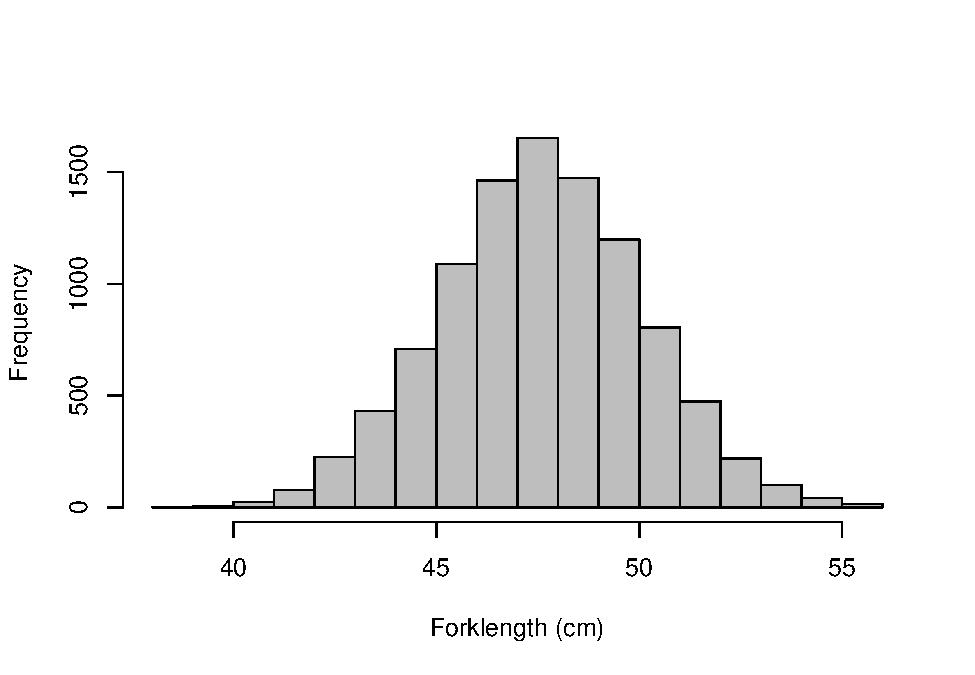
\includegraphics{worstr_files/figure-latex/unnamed-chunk-83-1.pdf}
We've add a couple of new arguments to the histogram call to make it a little less ugly here. In \protect\hyperlink{Chapter4}{Chapter 4} we are going to ramp it up and play with some plots!

\hypertarget{next3}{%
\section{Next steps}\label{next3}}

In this chapter, we provided a general overview of our work flow when it comes to reading in data and manipulating them to get useful summaries. In \protect\hyperlink{Chapter4}{Chapter 4} we will use these processes to help us visualize important trends in these summaries before we begin working with descriptive statistics and sampling distributions in \protect\hyperlink{Chapter5}{Chapter 5}.

\hypertarget{Chapter4}{%
\chapter{Plotting and graphics}\label{Chapter4}}

Sweet graphs, right? Want to learn how to make them? Okay, but baby steps here, alright?.

In this Chapter we will walk through plotting in R, both with the base graphic utilities that come with R, and the \texttt{ggplot2} package from the \texttt{tidyverse} that has taken over the world (er, revolutionized how we write R code). Both of these are actually great to work with for different reasons. The base graphics are built-in, powerful, and give you 100\% full control over your graphic environment. The \texttt{ggplot2} library (and a million packages that people have written to work with it) takes these to a new level in terms of functionality and 95\% of the time it will do exactly what you need. That other 5\% of the time it is really great to be able to fall back on the base graphics.

For the examples in this chapter, we'll work with the water quality data contained in \texttt{physical.csv}. You will need to download the class data sets that go with this book to play along if you have not already (click \href{https://danstich.github.io/stich/classes/BIOL217/software.html}{here} for instructions from the course website). But, you should have downloaded those to complete the examples in \protect\hyperlink{Chapter2}{Chapter 2}.

We will walk through histograms, scatter plots, line graphs, and boxplots in base graphics and \texttt{ggplot2} in this Chapter. Later in the book, we will add examples of how to plot predictions from statistical models alongside raw data using these same tools.

If you installed the \texttt{tidyverse} successfully in \protect\hyperlink{tidyverse}{Chapter 3}, then you can load all the packages we'll need by including \texttt{library(tidyverse)} at the start of your script:

\begin{Shaded}
\begin{Highlighting}[]
\CommentTok{# Chapter 4 Lecture module}

\CommentTok{# Package load}
\KeywordTok{library}\NormalTok{(tidyverse) }

\CommentTok{# 4.2 Plotting with base R ----}
\CommentTok{# ...}
\end{Highlighting}
\end{Shaded}

\hypertarget{plots-matter-as-much-as-stats}{%
\section{Plots matter as much as stats}\label{plots-matter-as-much-as-stats}}

Before we get started:

\begin{enumerate}
\def\labelenumi{\arabic{enumi}.}
\item
  There are few statistical tests that hold intuitive meaning to our readers. The ability to present information in a visually meaningful way to the reader can help to make the interpretation of your science crystal clear without having to worry about whether or not your reader has the faculties to interpret the results of some fancy statistical test that \emph{you} think is cool.
\item
  Effects and effect sizes are often (if not always) more important than the ability to detect `significant' differences. If you can present clear evidence that some treatment or manipulation confers a biologically meaningful change in a visual way alongside these tests, you can provide a much stronger body of evidence with which to argue your case.
\item
  There are a few graphical tools that are very useful for basic data exploration, diagnostics, etc., that can make your life a lot easier for data analysis and interpretation. They can also help you decide whether something has gone terribly wrong.
\end{enumerate}

The takeaway here is: \emph{don't make shitty graphs}.

\hypertarget{base-graphics}{%
\section{Plotting with base R}\label{base-graphics}}

Let's look at a few simple types of plots in R. The default graphics in R are not much to look at. But, there are a \textbf{ton} of ways to modify these plots, and the user (that's you!) can build plots from the ground up if needed.

One of the great things about base graphics is that many of the plot types take the same, or similar arguments that are all based on shared graphical parameters.

You can access the help file for these shared graphical parameters by running \texttt{?pars} in the console. We will use many of these in the sections that follow.

\hypertarget{histograms}{%
\subsection{Histograms}\label{histograms}}

Let's start with the histogram function that we began playing with at the end of \protect\hyperlink{stochastic}{Chapter 3}.

The \texttt{hist()} function plots a histogram but it actually does a whole lot more than just that. Like other plotting utilities, it can take a wide variety of arguments and it actually does some basic data analysis behind the scenes. All of the arguments are optional or have default values with the exception of the data that we want to plot (a numeric variable). This is the case for most plotting functions in the base graphics for R.

Start by reading in the data contained within the \texttt{physical.csv} file from the class data folder. Remember, I am assuming that your code is inside of a folder that also contains your class data folder that you named \href{https://danstich.github.io/stich/classes/BIOL217/software.html}{\texttt{data}}.

\begin{Shaded}
\begin{Highlighting}[]
\CommentTok{# I added stringsAsFactors = FALSE to read in all}
\CommentTok{# text strings as `chr`.}
\NormalTok{ otsego <-}\StringTok{ }\KeywordTok{read.csv}\NormalTok{(}\StringTok{"data/physical.csv"}\NormalTok{, }\DataTypeTok{stringsAsFactors =} \OtherTok{FALSE}\NormalTok{)}
\end{Highlighting}
\end{Shaded}

These are data collected each year from Otsego Lake by students, staff, and faculty at the SUNY Oneonta Biological Field Station in Cooperstown, NY, USA. The data set includes temperature (°C), pH, dissolved oxygen, and specific conductance measurements from a period of about 40 years. There are all kinds of cool spatial and seasonal patterns in the data that we can look at. We will use \texttt{temperature} for the examples that follow.

Make a histogram of temperature across all depths and dates just to see what we are working with here:

\begin{Shaded}
\begin{Highlighting}[]
\KeywordTok{hist}\NormalTok{(otsego}\OperatorTok{$}\NormalTok{temp)}
\end{Highlighting}
\end{Shaded}

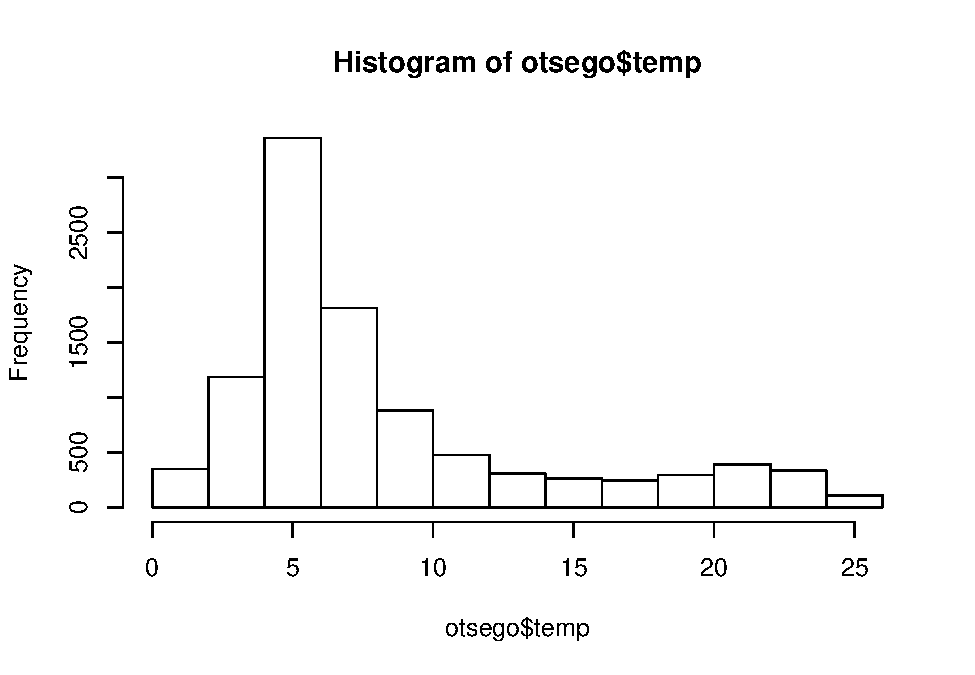
\includegraphics{worstr_files/figure-latex/unnamed-chunk-86-1.pdf}

The default histogram in base graphics leaves much to be desired. Thankfully, it is easy to modify the look of these figures. For example, we can add labels to the x and y-axis using \texttt{xlab} and \texttt{ylab}, and we can give the histogram a meaningful title by adding \texttt{main\ =\ ...} to the \texttt{hist()} call or remove it completely by saying \texttt{main\ =\ ""}.

\begin{Shaded}
\begin{Highlighting}[]
\KeywordTok{hist}\NormalTok{(otsego}\OperatorTok{$}\NormalTok{temp, }\DataTypeTok{xlab =} \StringTok{"Temperature"}\NormalTok{, }\DataTypeTok{ylab =} \StringTok{"Frequency"}\NormalTok{, }\DataTypeTok{main=}\StringTok{""}\NormalTok{)}
\end{Highlighting}
\end{Shaded}

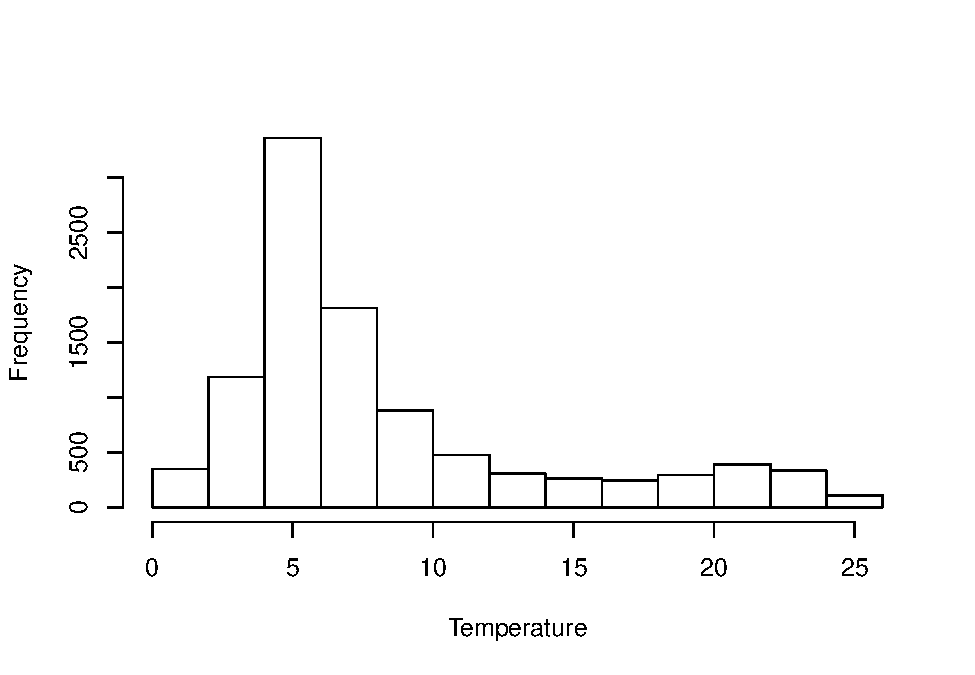
\includegraphics{worstr_files/figure-latex/unnamed-chunk-87-1.pdf}

We can make the axes cross at zero if we are concerned about that. We need to do this by specifying \texttt{yaxt\ =\ "n"}, \texttt{xaxt\ =\ "n"} in the \texttt{hist()} call and then follow up by telling R exactly where to start each of the axes. In this example, I also add some changes to the color of the bars (\texttt{col}) and the color of the borders (\texttt{border}). Finally, I fix the x- and y-axis scales so I know where they'll start.

\begin{Shaded}
\begin{Highlighting}[]
\CommentTok{# Make the histogram}
\KeywordTok{hist}\NormalTok{(otsego}\OperatorTok{$}\NormalTok{temp,}
     \DataTypeTok{xlab =} \StringTok{"Temperature"}\NormalTok{,}
     \DataTypeTok{ylab =} \StringTok{"Frequency"}\NormalTok{,}
     \DataTypeTok{main =} \StringTok{""}\NormalTok{,}
     \DataTypeTok{xaxt =} \StringTok{"n"}\NormalTok{,}
     \DataTypeTok{yaxt =} \StringTok{"n"}\NormalTok{,}
     \DataTypeTok{col =} \StringTok{"gray87"}\NormalTok{,}
     \DataTypeTok{border =} \StringTok{"white"}\NormalTok{,}
     \DataTypeTok{xlim =} \KeywordTok{c}\NormalTok{(}\DecValTok{0}\NormalTok{, }\DecValTok{30}\NormalTok{),}
     \DataTypeTok{ylim =} \KeywordTok{c}\NormalTok{(}\DecValTok{0}\NormalTok{, }\DecValTok{3500}\NormalTok{)}
\NormalTok{     )}

\CommentTok{# Add an x-axis going from zero to thirty degrees}
\CommentTok{# in increments of 2 degrees and start it at zero}
\KeywordTok{axis}\NormalTok{(}\DataTypeTok{side =} \DecValTok{1}\NormalTok{, }\DataTypeTok{at =} \KeywordTok{seq}\NormalTok{(}\DataTypeTok{from =} \DecValTok{0}\NormalTok{, }\DataTypeTok{to =} \DecValTok{30}\NormalTok{, }\DataTypeTok{by =} \DecValTok{2}\NormalTok{), }\DataTypeTok{pos =} \DecValTok{0}\NormalTok{)}

\CommentTok{# Add a rotated y-axis with default scale and }
\CommentTok{# start it at zero}
\KeywordTok{axis}\NormalTok{(}\DataTypeTok{side =} \DecValTok{2}\NormalTok{, }\DataTypeTok{las =} \DecValTok{2}\NormalTok{, }\DataTypeTok{pos =} \DecValTok{0}\NormalTok{)}
\end{Highlighting}
\end{Shaded}

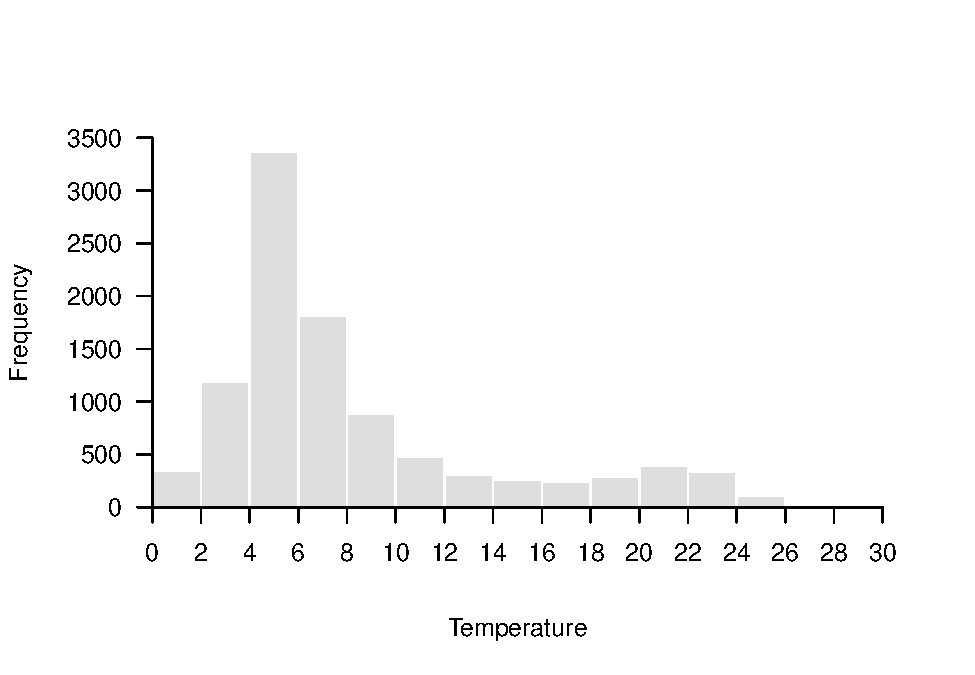
\includegraphics{worstr_files/figure-latex/unnamed-chunk-88-1.pdf}

\textbf{Colors!!!}

If \texttt{gray87} is not your style (whatevs), there are another 656 pre-named colors in R. You can see their names by running \texttt{colors()} in the console like this:

\begin{Shaded}
\begin{Highlighting}[]
\KeywordTok{colors}\NormalTok{()}
\end{Highlighting}
\end{Shaded}

If you are a little more adventurous, you might try the \texttt{rgb()} color specification or hex values. I really like the \texttt{rgb()} specification because you can include an \texttt{alpha} channel to make your colors transparent (oooooh!). For example, if I change my code above to use the following:

\begin{Shaded}
\begin{Highlighting}[]
\NormalTok{col =}\StringTok{ }\KeywordTok{rgb}\NormalTok{(}\DataTypeTok{red =} \FloatTok{0.90}\NormalTok{, }\DataTypeTok{green =} \DecValTok{0}\NormalTok{, }\DataTypeTok{blue =} \FloatTok{0.30}\NormalTok{, }\DataTypeTok{alpha =} \FloatTok{0.10}\NormalTok{)}
\end{Highlighting}
\end{Shaded}

I get a transparent, purple histogram.

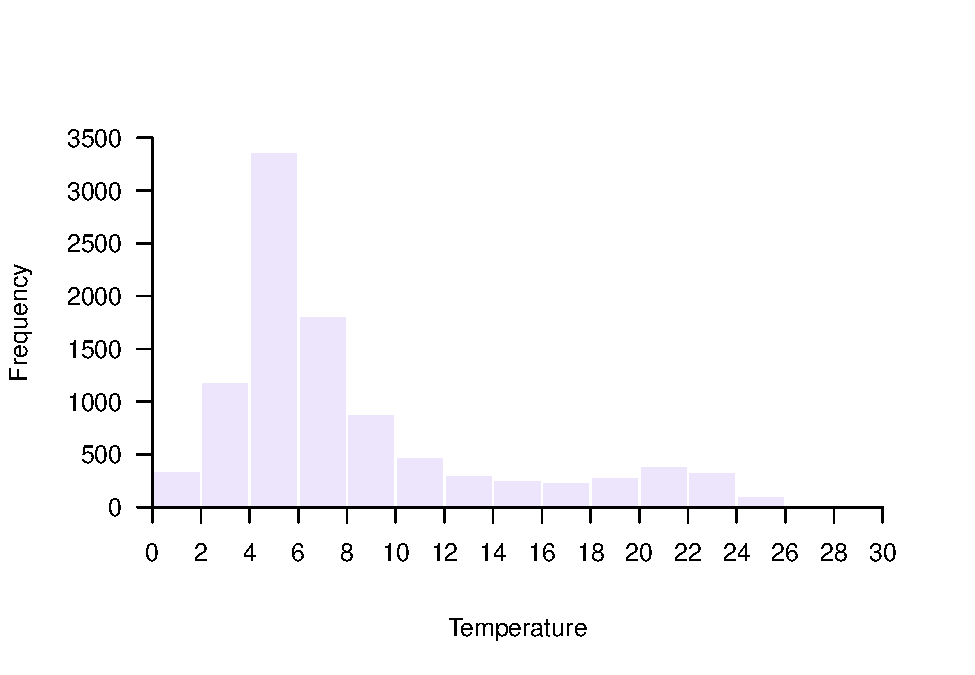
\includegraphics{worstr_files/figure-latex/unnamed-chunk-91-1.pdf}

So purply.

There are tons of great blogs and eBooks with whole chapters devoted to colors and color palletes in R. There are even whole packages we'll work with dedicated to colors. By all means, check them out! We will work with a few as we continue to increase complexity.

\hypertarget{scatterplots}{%
\subsection{Scatterplots}\label{scatterplots}}

Scatter plots are a great starting point for doing exploratory data analysis or for displaying raw data along with summary graphics. They are also the default behavior for the \texttt{plot()} function for continuous variables in base R.

Let's demonstrate by by plotting surface temperature (\texttt{depth} = 0.1 m) by month across years. We'll use the data management skills we picked up in \protect\hyperlink{Chapterux5cux25203}{Chapter 3} to filter the data first.

\begin{Shaded}
\begin{Highlighting}[]
\CommentTok{# Filter to get July surface temperatures}
\NormalTok{surface <-}\StringTok{ }\NormalTok{otsego }\OperatorTok\StringTok{ }\KeywordTok{filter}\NormalTok{(depth }\OperatorTok{==}\StringTok{ }\FloatTok{0.1}\NormalTok{)}

\CommentTok{# Default scatter plot}
\KeywordTok{plot}\NormalTok{(}\DataTypeTok{x =}\NormalTok{ surface}\OperatorTok{$}\NormalTok{month, }\DataTypeTok{y =}\NormalTok{ surface}\OperatorTok{$}\NormalTok{temp)}
\end{Highlighting}
\end{Shaded}

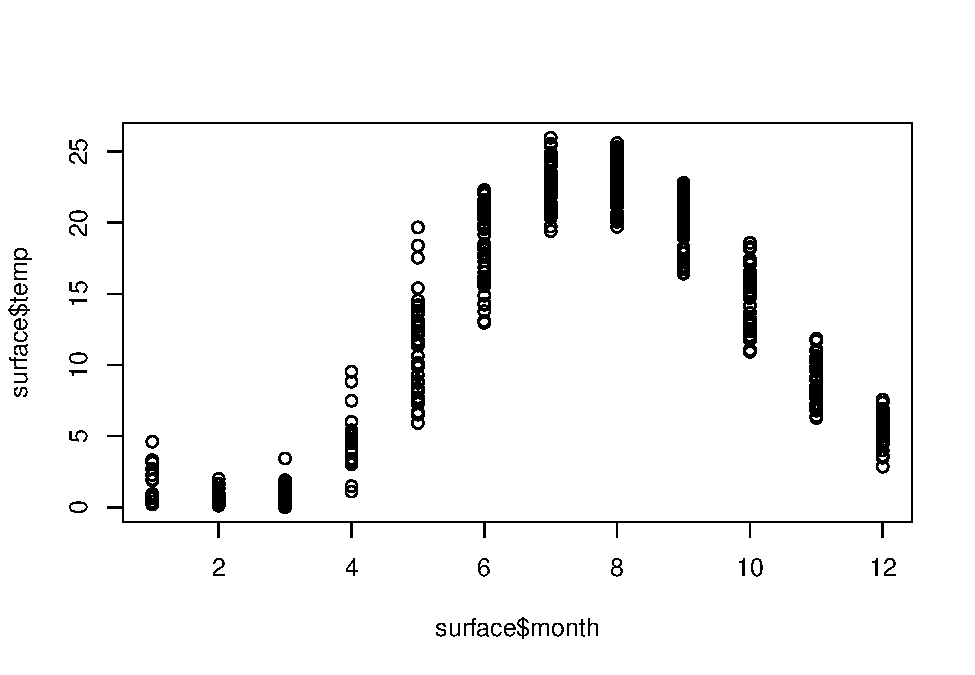
\includegraphics{worstr_files/figure-latex/unnamed-chunk-92-1.pdf}

As with the \texttt{hist()} function, the default here is underwhelming. We can use many of the same arguments that we specified in \texttt{hist()} to dress this up a bit. This time, we will specify a plotting character \texttt{pch} that corresponds to a filled circle. Then, we tell R to give it an \texttt{rgb()} background (\texttt{bg}) with no color for lines that go around each point. That way the data points are darker where there is overlap between them. Finally, we use \texttt{expression()} to include the degree symbol in the y-axis label.

\begin{Shaded}
\begin{Highlighting}[]
\CommentTok{# Better scatter plot}
\KeywordTok{plot}\NormalTok{(}\DataTypeTok{x =}\NormalTok{ surface}\OperatorTok{$}\NormalTok{month, }
     \DataTypeTok{y =}\NormalTok{ surface}\OperatorTok{$}\NormalTok{temp,}
     \DataTypeTok{pch =} \DecValTok{21}\NormalTok{,}
     \DataTypeTok{bg =} \KeywordTok{rgb}\NormalTok{(}\DecValTok{0}\NormalTok{, }\DecValTok{0}\NormalTok{, }\DecValTok{0}\NormalTok{, }\FloatTok{0.2}\NormalTok{),}
     \DataTypeTok{col =} \OtherTok{NA}\NormalTok{,}
     \DataTypeTok{xlab =} \StringTok{"Month"}\NormalTok{,}
     \DataTypeTok{ylab =} \KeywordTok{expression}\NormalTok{(}\KeywordTok{paste}\NormalTok{(}\StringTok{"Temperature ( "}\NormalTok{, degree, }\StringTok{"C)"}\NormalTok{))}
\NormalTok{     )}
\end{Highlighting}
\end{Shaded}

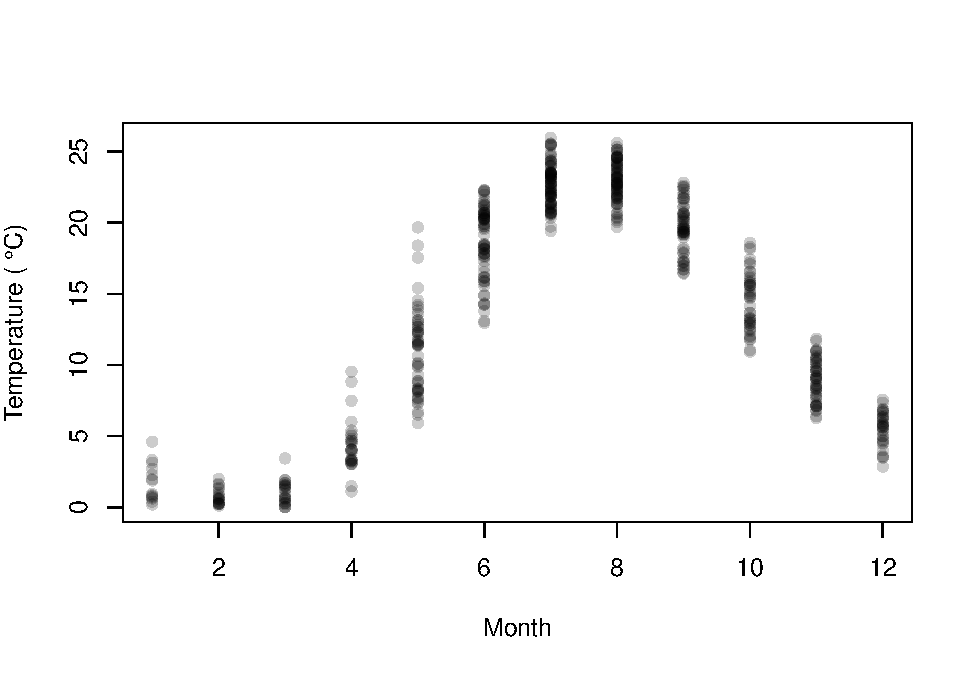
\includegraphics{worstr_files/figure-latex/unnamed-chunk-93-1.pdf}

This is a lot more informative because it shows us where most of the observations fall within a given month, and how much variability there is. But, it would be nice to have some summary.

\hypertarget{lines}{%
\subsection{Lines}\label{lines}}

We can plot lines in a few different ways in the base graphics of R. We can create stand-alone line graphs with data in R pretty easily with the \texttt{plot()} function we used for scatter plots in the preceding section.

For example, let's say that we want to just plot average surface temperature in each month as a line graph. We can summarize the data quickly and then plot those:

\begin{Shaded}
\begin{Highlighting}[]
\NormalTok{mids <-}\StringTok{ }\NormalTok{surface }\OperatorTok
\StringTok{  }\KeywordTok{group_by}\NormalTok{(month) }\OperatorTok
\StringTok{  }\KeywordTok{summarize}\NormalTok{(}\DataTypeTok{avg =} \KeywordTok{mean}\NormalTok{(temp))}

\KeywordTok{plot}\NormalTok{(mids}\OperatorTok{$}\NormalTok{month, mids}\OperatorTok{$}\NormalTok{avg, }\DataTypeTok{type =} \StringTok{"l"}\NormalTok{, }\DataTypeTok{xlab =} \StringTok{"Month"}\NormalTok{, }\DataTypeTok{ylab =} \StringTok{"Average"}\NormalTok{)}
\end{Highlighting}
\end{Shaded}

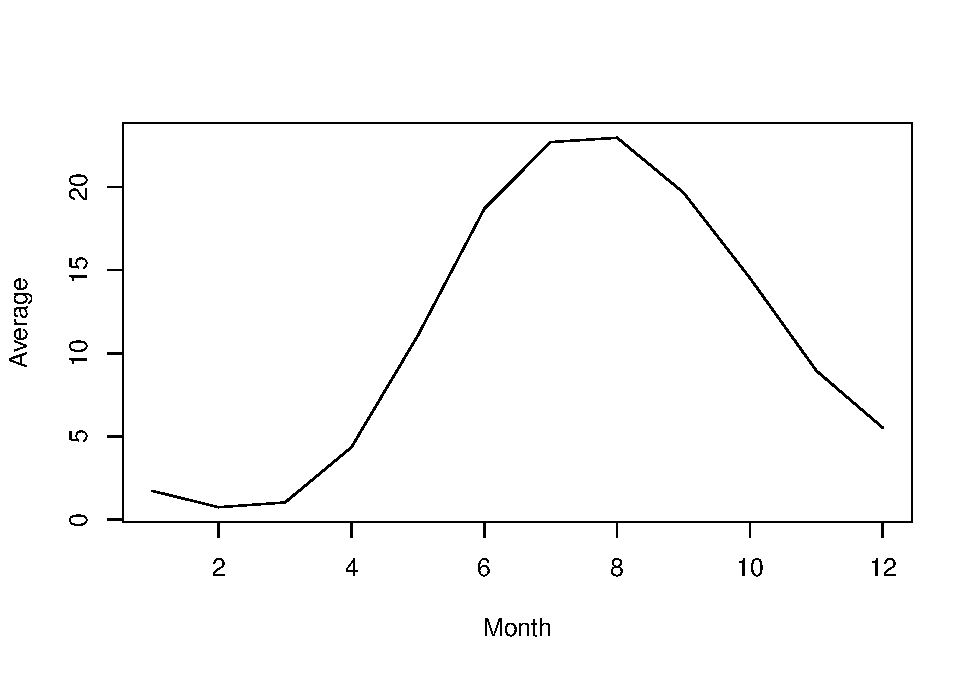
\includegraphics{worstr_files/figure-latex/unnamed-chunk-94-1.pdf}

We could even add these to the scatter plot of our raw data using the \texttt{lines()} function. Play around with \texttt{lty} and \texttt{lwd} to see if you can figure out what they do. If you get stuck, don't forget to Google it! (Worst Stats Text eveR.)

\begin{Shaded}
\begin{Highlighting}[]
\CommentTok{# Same scatter plot}
\KeywordTok{plot}\NormalTok{(}\DataTypeTok{x =}\NormalTok{ surface}\OperatorTok{$}\NormalTok{month, }
     \DataTypeTok{y =}\NormalTok{ surface}\OperatorTok{$}\NormalTok{temp,}
     \DataTypeTok{pch =} \DecValTok{21}\NormalTok{,}
     \DataTypeTok{bg =} \KeywordTok{rgb}\NormalTok{(}\DecValTok{0}\NormalTok{, }\DecValTok{0}\NormalTok{, }\DecValTok{0}\NormalTok{, }\FloatTok{0.2}\NormalTok{),}
     \DataTypeTok{col =} \OtherTok{NA}\NormalTok{,}
     \DataTypeTok{xlab =} \StringTok{"Month"}\NormalTok{,}
     \DataTypeTok{ylab =} \KeywordTok{expression}\NormalTok{(}\KeywordTok{paste}\NormalTok{(}\StringTok{"Temperature ( "}\NormalTok{, degree, }\StringTok{"C)"}\NormalTok{))}
\NormalTok{     )}
\CommentTok{# Add a thick, dotted line that is gray (this is a gray40 job)}
\KeywordTok{lines}\NormalTok{(mids}\OperatorTok{$}\NormalTok{month, mids}\OperatorTok{$}\NormalTok{avg, }\DataTypeTok{lty =} \DecValTok{3}\NormalTok{, }\DataTypeTok{lwd =} \DecValTok{2}\NormalTok{, }\DataTypeTok{col =} \StringTok{"gray40"}\NormalTok{)}
\end{Highlighting}
\end{Shaded}

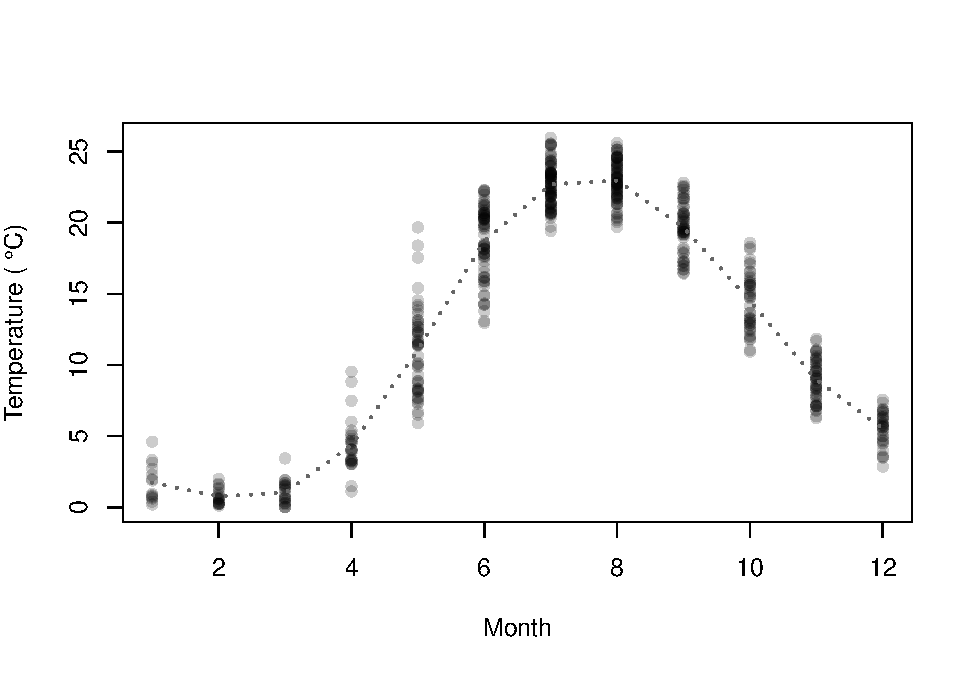
\includegraphics{worstr_files/figure-latex/unnamed-chunk-95-1.pdf}

We could also add the means to the main plot with \texttt{points()} and choose a different size or color than the raw data. We'll look at these options and more as we step up complexity.

For raw data like these, though, we are better off using a box plot to show those types of summaries.

\hypertarget{boxplots}{%
\subsection{Boxplots}\label{boxplots}}

The basic box plot is straightforward to create, but can be a real pain to modify because the syntax is slightly different from the other plotting functions we've worked with so far.

Let's try to summarize surface temperature by month using a box plot to see how these work in the base R graphics. Notice that we are specifying the variables as a formula here, and explicitly telling R what the data set is:

\begin{Shaded}
\begin{Highlighting}[]
\KeywordTok{boxplot}\NormalTok{(temp}\OperatorTok{~}\NormalTok{month, }\DataTypeTok{data =}\NormalTok{ surface,}
        \DataTypeTok{xlab =} \StringTok{"Month"}\NormalTok{,}
        \DataTypeTok{ylab =} \KeywordTok{expression}\NormalTok{(}\KeywordTok{paste}\NormalTok{(}\StringTok{"Surface temperature ( "}\NormalTok{, degree, }\StringTok{"C)"}\NormalTok{)))}
\end{Highlighting}
\end{Shaded}

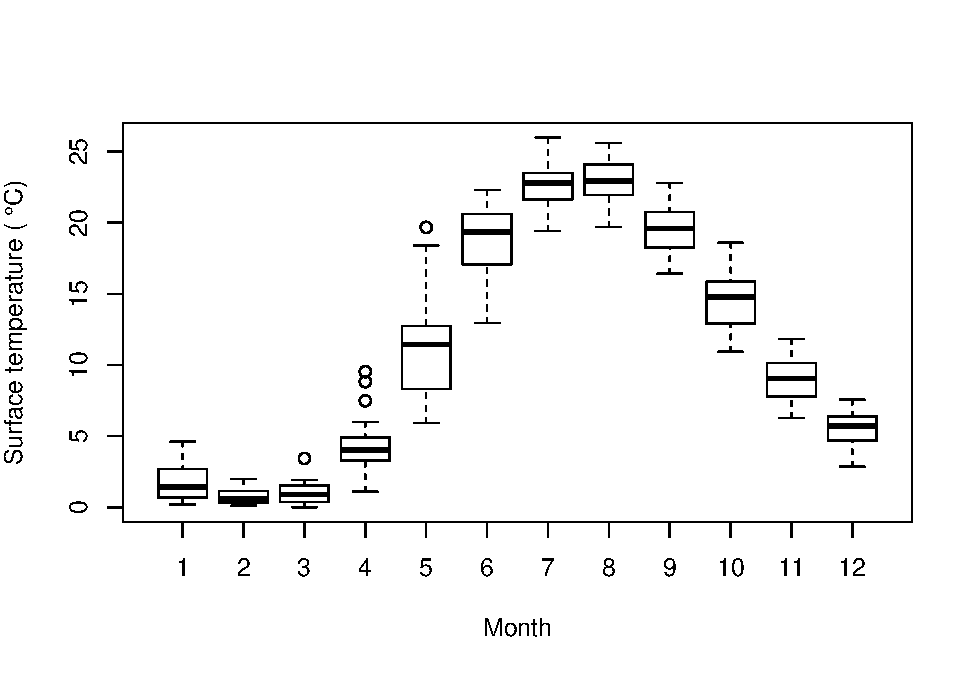
\includegraphics{worstr_files/figure-latex/unnamed-chunk-96-1.pdf}

Wow, that was waaaaay to easy! Have you ever tried to make one of those in Excel? Forget about it. It would take you half a day, and then when you realized you forgot ten data points you would have to do it all again.

But, it is still much ugly. Maybe there is a way we can change that?

Of course there is!

Let's add a little color and tweak some options. For a full set of optional arguments you can change, run \texttt{?bxp} in the console. (Ooh, that one is sneaky: \texttt{bxp()} is the function inside of \texttt{boxplot()} that actually draws the plots).

Options are named consistently by the part of the plot. For example, \texttt{boxwex}, \texttt{boxcol} and \texttt{boxfill} all control the look of the box. Likewise, the options \texttt{boxcol}, \texttt{whiskcol} and \texttt{staplecol} control the colors of the box, whiskers, and staples, respectively. Nifty, right? Play with the settings below to see what each one does. Then, go explore some more options.It is the easiest way to learn when you are learning from The Worst Stats Text eveR.

\begin{Shaded}
\begin{Highlighting}[]
\KeywordTok{boxplot}\NormalTok{(temp}\OperatorTok{~}\NormalTok{month, }
        \DataTypeTok{data =}\NormalTok{ surface,}
        \DataTypeTok{xlab =} \StringTok{"Month"}\NormalTok{,}
        \DataTypeTok{ylab =} \KeywordTok{expression}\NormalTok{(}\KeywordTok{paste}\NormalTok{(}\StringTok{"Surface temperature ( "}\NormalTok{, degree, }\StringTok{"C)"}\NormalTok{)),      }
        \DataTypeTok{border =} \StringTok{"gray40"}\NormalTok{,}
        \DataTypeTok{boxwex =} \FloatTok{0.50}\NormalTok{, }\DataTypeTok{boxcol =} \StringTok{"gray40"}\NormalTok{, }\DataTypeTok{boxfill =} \StringTok{"gray87"}\NormalTok{,}
        \DataTypeTok{whisklty =} \DecValTok{1}\NormalTok{, }\DataTypeTok{whisklwd=}\DecValTok{1}\NormalTok{, }\DataTypeTok{whiskcol =} \StringTok{"gray40"}\NormalTok{,}
        \DataTypeTok{staplewex =} \DecValTok{0}\NormalTok{, }\DataTypeTok{staplecol =} \OtherTok{NA}\NormalTok{,}
        \DataTypeTok{outpch =} \DecValTok{21}\NormalTok{, }\DataTypeTok{outbg =} \StringTok{"gray90"}\NormalTok{, }\DataTypeTok{outcol =} \StringTok{"gray90"}
\NormalTok{        )}
\end{Highlighting}
\end{Shaded}

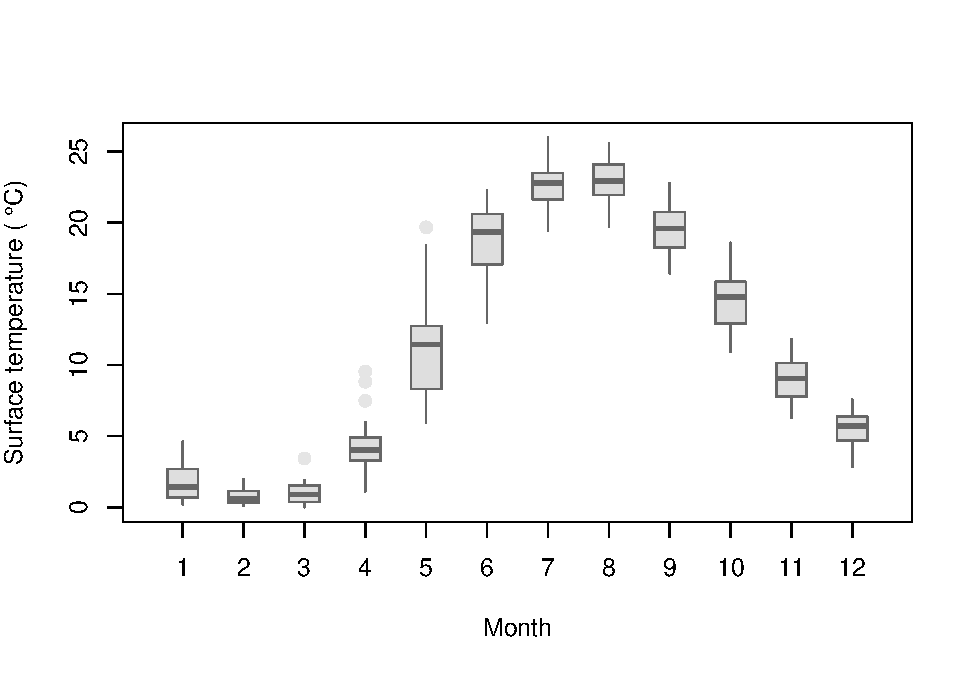
\includegraphics{worstr_files/figure-latex/unnamed-chunk-97-1.pdf}

Finally, we can combine this with a scatter plot to \texttt{jitter} our raw data over the top of the boxes in each month:

\begin{Shaded}
\begin{Highlighting}[]
\KeywordTok{boxplot}\NormalTok{(temp}\OperatorTok{~}\NormalTok{month, }
        \DataTypeTok{data =}\NormalTok{ surface,}
        \DataTypeTok{xlab =} \StringTok{"Month"}\NormalTok{,}
        \DataTypeTok{ylab =} \KeywordTok{expression}\NormalTok{(}\KeywordTok{paste}\NormalTok{(}\StringTok{"Surface temperature ( "}\NormalTok{, degree, }\StringTok{"C)"}\NormalTok{)),      }
        \DataTypeTok{border =} \StringTok{"gray40"}\NormalTok{,}
        \DataTypeTok{boxwex =} \FloatTok{0.50}\NormalTok{, }\DataTypeTok{boxcol =} \StringTok{"gray40"}\NormalTok{, }\DataTypeTok{boxfill =} \StringTok{"gray87"}\NormalTok{,}
        \DataTypeTok{whisklty =} \DecValTok{1}\NormalTok{, }\DataTypeTok{whisklwd=}\DecValTok{1}\NormalTok{, }\DataTypeTok{whiskcol =} \StringTok{"gray40"}\NormalTok{,}
        \DataTypeTok{staplewex =} \DecValTok{0}\NormalTok{, }\DataTypeTok{staplecol =} \OtherTok{NA}\NormalTok{,}
        \DataTypeTok{outpch =} \DecValTok{21}\NormalTok{, }\DataTypeTok{outbg =} \OtherTok{NA}\NormalTok{, }\DataTypeTok{outcol =} \OtherTok{NA}
\NormalTok{        )}
\KeywordTok{points}\NormalTok{(}\KeywordTok{jitter}\NormalTok{(surface}\OperatorTok{$}\NormalTok{month), surface}\OperatorTok{$}\NormalTok{temp, }\DataTypeTok{cex=}\NormalTok{.}\DecValTok{4}\NormalTok{, }\DataTypeTok{pch=}\DecValTok{19}\NormalTok{, }\DataTypeTok{col=}\KeywordTok{rgb}\NormalTok{(}\DecValTok{0}\NormalTok{,}\DecValTok{0}\NormalTok{,}\DecValTok{0}\NormalTok{,}\FloatTok{0.2}\NormalTok{))}
\end{Highlighting}
\end{Shaded}

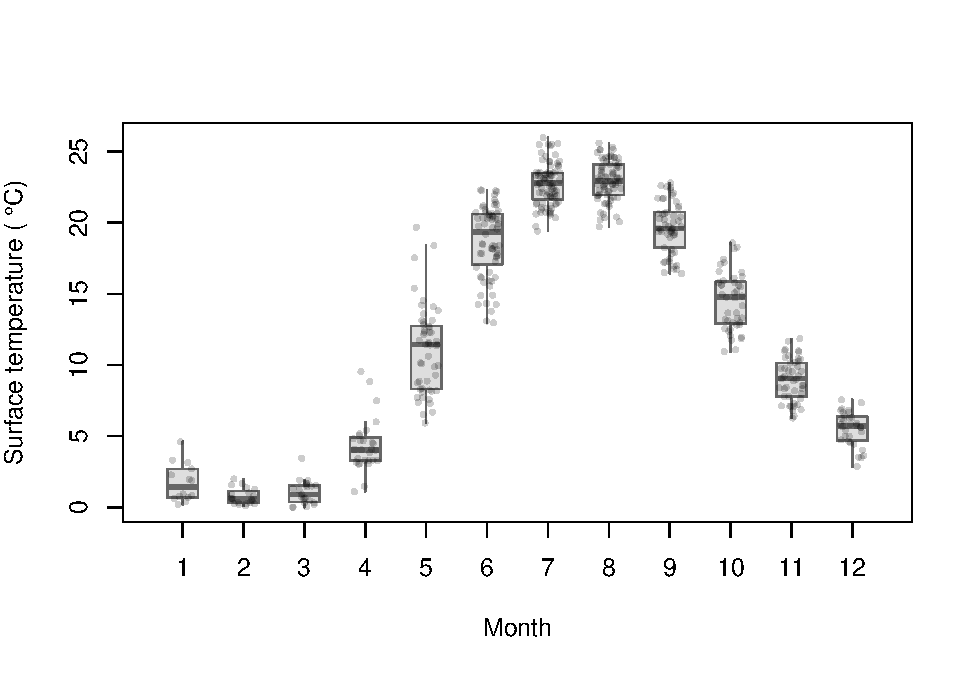
\includegraphics{worstr_files/figure-latex/unnamed-chunk-98-1.pdf}

That is actually starting to look pretty snazzy! We'll continue to work to improve our base graphics as we move forward. For now, let's have a look at how to do these things in \texttt{ggplot2} next.

\hypertarget{plotting-with-ggplot2}{%
\section{\texorpdfstring{Plotting with \texttt{ggplot2}}{Plotting with ggplot2}}\label{plotting-with-ggplot2}}

Plotting with \href{https://ggplot2.tidyverse.org/}{\texttt{ggplot2}} and the dozens of packages that use it is a bit different than plotting with base graphics in R. Part of the reason for this is that it uses a work flow that is similar to the data manipulation we have looked at so far. In general, you could think of this as creating a canvas, applying some routine aesthetics based on the data structure (e.g.~grouping), and then adding layers on to the canvas like we did with \protect\hyperlink{base-graphics}{base graphics}.

It takes a little getting used to, but you'll see how powerful it can be for multifaceted plots when we get to later chapters. We'll walk through the same plots that we did in \protect\hyperlink{base-graphics}{base graphics}, but this time we'll use the \texttt{ggplot()} function and layer on the pieces.

\hypertarget{gghists}{%
\subsection{Histograms}\label{gghists}}

The default histogram is easy to create with \texttt{ggplot()} and a geometry layer. We start with the \texttt{ggplot} call, and then add the histogram geometry, \texttt{geom\_histogram()}, like this. I usually save the plot to an object with an arbitrary name I don't use for anything, like \texttt{p} or \texttt{s} or \texttt{v}, and then print it explicitly.

\begin{Shaded}
\begin{Highlighting}[]
\CommentTok{# Histogram of water temperature across }
\CommentTok{# all dates and depths}
\NormalTok{p <-}\StringTok{ }\KeywordTok{ggplot}\NormalTok{(otsego, }\KeywordTok{aes}\NormalTok{(}\DataTypeTok{x=}\NormalTok{temp)) }\OperatorTok{+}\StringTok{ }\KeywordTok{geom_histogram}\NormalTok{(}\DataTypeTok{bins=}\DecValTok{30}\NormalTok{)}

\KeywordTok{print}\NormalTok{(p)}
\end{Highlighting}
\end{Shaded}

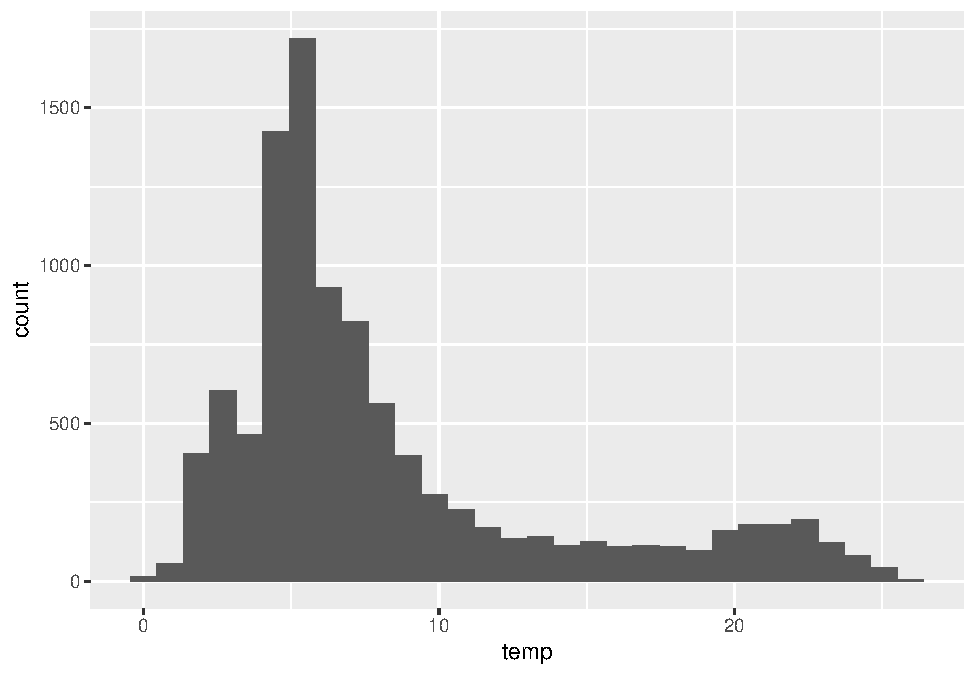
\includegraphics{worstr_files/figure-latex/unnamed-chunk-99-1.pdf}

Right away this looks a lot prettier than the default histogram that we produced with base graphics. Of course, we can customize just like we did before.

Let's add labels for the x and y-axis next:

\begin{Shaded}
\begin{Highlighting}[]
\CommentTok{# Histogram of water temperature across }
\CommentTok{# all dates and depths}
\NormalTok{p <-}\StringTok{ }\KeywordTok{ggplot}\NormalTok{(otsego, }\KeywordTok{aes}\NormalTok{(}\DataTypeTok{x=}\NormalTok{temp)) }\OperatorTok{+}\StringTok{ }
\StringTok{  }\KeywordTok{geom_histogram}\NormalTok{(}\DataTypeTok{bins=}\DecValTok{30}\NormalTok{) }\OperatorTok{+}\StringTok{ }
\StringTok{  }\KeywordTok{xlab}\NormalTok{(}\KeywordTok{expression}\NormalTok{(}\KeywordTok{paste}\NormalTok{(}\StringTok{"Temperature ("}\NormalTok{, degree, }\StringTok{"C)"}\NormalTok{))) }\OperatorTok{+}
\StringTok{  }\KeywordTok{ylab}\NormalTok{(}\StringTok{"Count"}\NormalTok{)}

\KeywordTok{print}\NormalTok{(p)}
\end{Highlighting}
\end{Shaded}

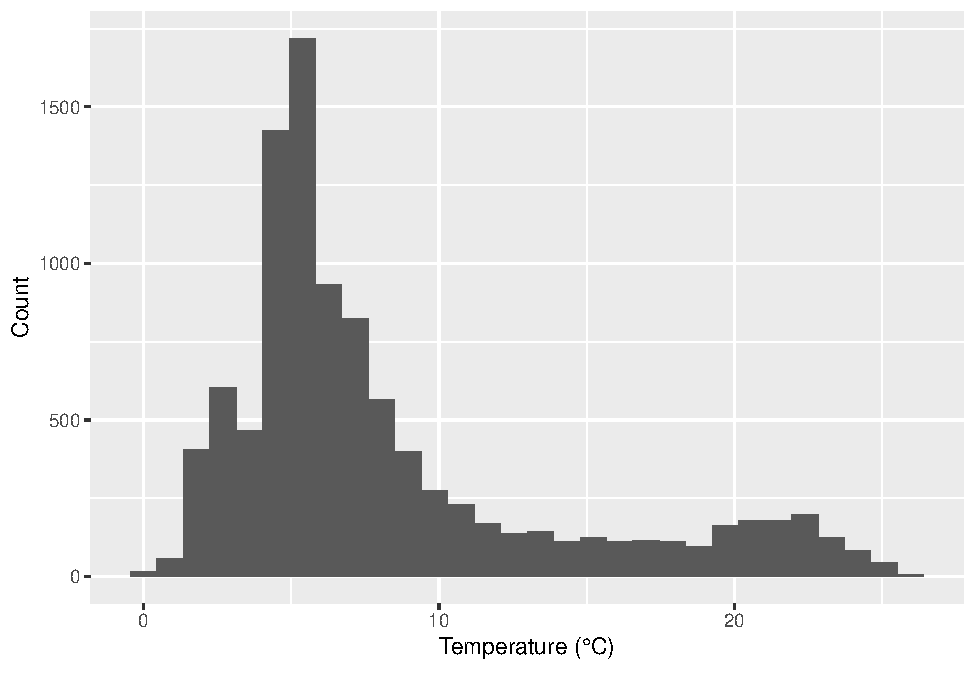
\includegraphics{worstr_files/figure-latex/unnamed-chunk-100-1.pdf}

We can also scale the \texttt{x-axis} and the \texttt{y-axis} like we did in the \protect\hyperlink{histograms}{base graphics example}.

\begin{Shaded}
\begin{Highlighting}[]
\CommentTok{# Histogram of water temperature across }
\CommentTok{# all dates and depths}
\NormalTok{p <-}\StringTok{ }\KeywordTok{ggplot}\NormalTok{(otsego, }\KeywordTok{aes}\NormalTok{(}\DataTypeTok{x=}\NormalTok{temp)) }\OperatorTok{+}\StringTok{ }
\StringTok{  }\KeywordTok{geom_histogram}\NormalTok{(}\DataTypeTok{bins=}\DecValTok{30}\NormalTok{) }\OperatorTok{+}\StringTok{ }
\StringTok{  }\KeywordTok{xlab}\NormalTok{(}\KeywordTok{expression}\NormalTok{(}\KeywordTok{paste}\NormalTok{(}\StringTok{"Temperature ("}\NormalTok{, degree, }\StringTok{"C)"}\NormalTok{))) }\OperatorTok{+}
\StringTok{  }\KeywordTok{ylab}\NormalTok{(}\StringTok{"Count"}\NormalTok{) }\OperatorTok{+}
\StringTok{  }\KeywordTok{scale_x_continuous}\NormalTok{(}\DataTypeTok{limits=}\KeywordTok{c}\NormalTok{(}\DecValTok{0}\NormalTok{, }\DecValTok{25}\NormalTok{), }\DataTypeTok{expand =} \KeywordTok{c}\NormalTok{(}\DecValTok{0}\NormalTok{, }\DecValTok{0}\NormalTok{)) }\OperatorTok{+}\StringTok{ }
\StringTok{  }\KeywordTok{scale_y_continuous}\NormalTok{(}\DataTypeTok{expand =} \KeywordTok{c}\NormalTok{(}\DecValTok{0}\NormalTok{, }\DecValTok{0}\NormalTok{))}
\KeywordTok{print}\NormalTok{(p)}
\end{Highlighting}
\end{Shaded}

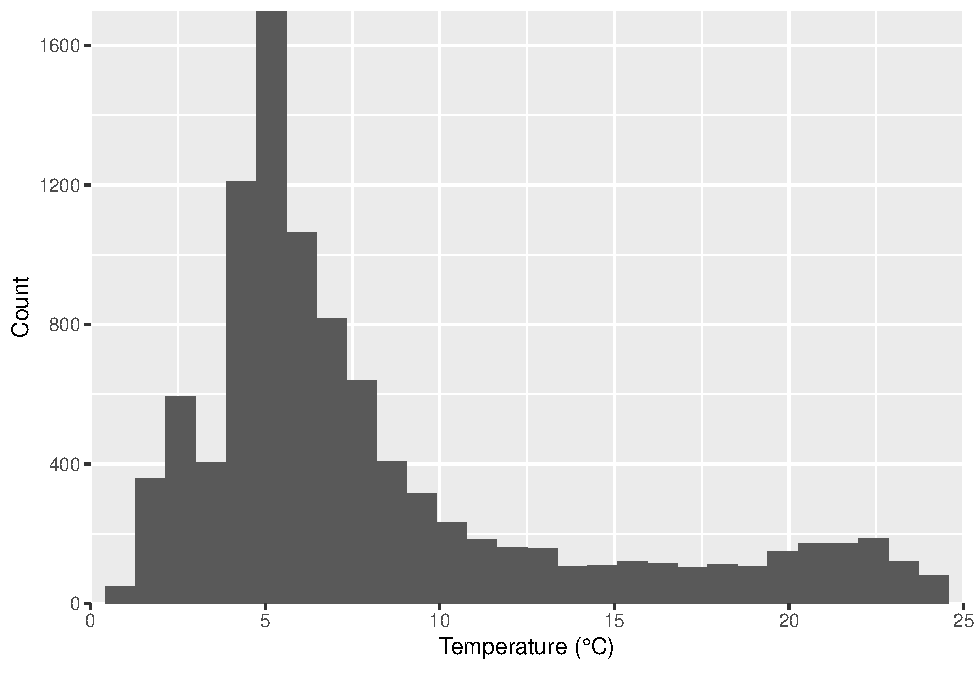
\includegraphics{worstr_files/figure-latex/unnamed-chunk-101-1.pdf}

We can modify each of other layers individually, all at once using preset ggplot \href{http://www.sthda.com/english/wiki/ggplot2-title-main-axis-and-legend-titles}{themes} or by modifying a pre-defined theme.

Let's have a look at how a theme changes the appearance. I am going to add \texttt{theme\_bw()} here, but check out the others linked above. I also add a few adjust the position of the x- and y-axis labels and removed the panel grid in the \texttt{theme()} function after applying a theme.

\begin{Shaded}
\begin{Highlighting}[]
\CommentTok{# Histogram of water temperature across }
\CommentTok{# all dates and depths}
\NormalTok{p <-}\StringTok{ }\KeywordTok{ggplot}\NormalTok{(otsego, }\KeywordTok{aes}\NormalTok{(}\DataTypeTok{x=}\NormalTok{temp)) }\OperatorTok{+}\StringTok{ }
\StringTok{  }\KeywordTok{geom_histogram}\NormalTok{(}\DataTypeTok{bins=}\DecValTok{30}\NormalTok{) }\OperatorTok{+}\StringTok{ }
\StringTok{  }\KeywordTok{scale_x_continuous}\NormalTok{(}\DataTypeTok{limits=}\KeywordTok{c}\NormalTok{(}\DecValTok{0}\NormalTok{, }\DecValTok{25}\NormalTok{), }\DataTypeTok{expand =} \KeywordTok{c}\NormalTok{(}\DecValTok{0}\NormalTok{, }\DecValTok{0}\NormalTok{)) }\OperatorTok{+}\StringTok{ }
\StringTok{  }\KeywordTok{scale_y_continuous}\NormalTok{(}\DataTypeTok{expand =} \KeywordTok{c}\NormalTok{(}\DecValTok{0}\NormalTok{, }\DecValTok{0}\NormalTok{)) }\OperatorTok{+}\StringTok{ }
\StringTok{  }\KeywordTok{xlab}\NormalTok{(}\KeywordTok{expression}\NormalTok{(}\KeywordTok{paste}\NormalTok{(}\StringTok{"Temperature ("}\NormalTok{, degree, }\StringTok{"C)"}\NormalTok{))) }\OperatorTok{+}
\StringTok{  }\KeywordTok{ylab}\NormalTok{(}\StringTok{"Count"}\NormalTok{) }\OperatorTok{+}
\StringTok{  }\KeywordTok{theme_bw}\NormalTok{() }\OperatorTok{+}
\StringTok{  }\KeywordTok{theme}\NormalTok{(}
    \DataTypeTok{axis.title.x =} \KeywordTok{element_text}\NormalTok{(}\DataTypeTok{vjust =} \DecValTok{-1}\NormalTok{),}
    \DataTypeTok{axis.title.y =} \KeywordTok{element_text}\NormalTok{(}\DataTypeTok{vjust =} \DecValTok{3}\NormalTok{),}
    \DataTypeTok{panel.grid =} \KeywordTok{element_blank}\NormalTok{()}
\NormalTok{  )}
\KeywordTok{print}\NormalTok{(p)}
\end{Highlighting}
\end{Shaded}

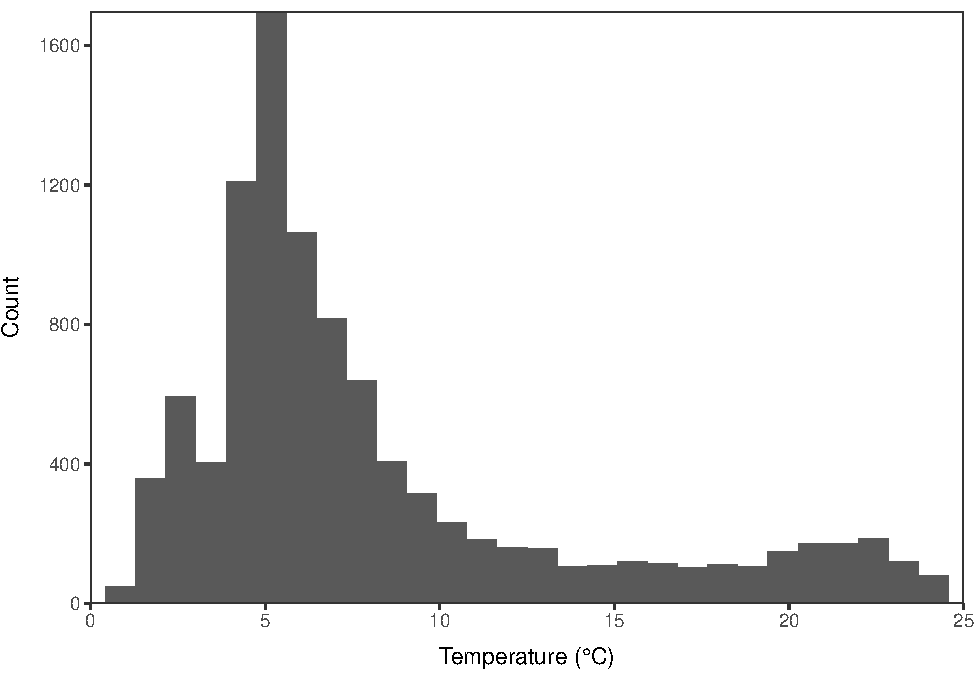
\includegraphics{worstr_files/figure-latex/unnamed-chunk-102-1.pdf}

Spend some time practicing this and changing options to see what you can come up with. Be sure to check out the descriptions of the options you can pass to theme by running \texttt{?theme} to get the help file.

\hypertarget{ggscatter}{%
\subsection{Scatter plots}\label{ggscatter}}

Now that we have a basic feel for the \texttt{ggplot2} work flow, changing plot types is really easy because all of the parts of our plots work together in the same way.

As a reminder, we previously built scatter plots of surface temperature in Otsego Lake, NY by month using base graphics.

Go ahead and subset the data again:

\begin{Shaded}
\begin{Highlighting}[]
\NormalTok{surface <-}\StringTok{ }\NormalTok{otsego }\OperatorTok\StringTok{ }\KeywordTok{filter}\NormalTok{(depth }\OperatorTok{==}\StringTok{ }\FloatTok{0.10}\NormalTok{)}
\end{Highlighting}
\end{Shaded}

Now, we can make the default scatterplot:

\begin{Shaded}
\begin{Highlighting}[]
\NormalTok{s <-}\StringTok{ }\KeywordTok{ggplot}\NormalTok{(surface, }\KeywordTok{aes}\NormalTok{(}\DataTypeTok{x =}\NormalTok{ month, }\DataTypeTok{y =}\NormalTok{ temp)) }\OperatorTok{+}
\StringTok{  }\KeywordTok{geom_point}\NormalTok{()}
\KeywordTok{print}\NormalTok{(s)}
\end{Highlighting}
\end{Shaded}

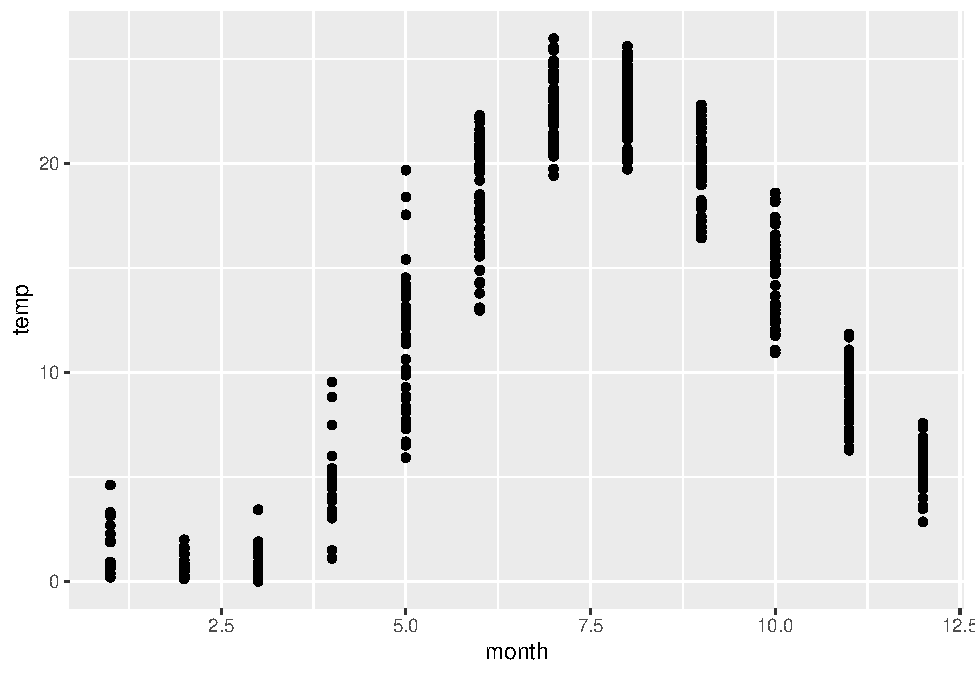
\includegraphics{worstr_files/figure-latex/unnamed-chunk-104-1.pdf}

At a glance, this already looks a lot nicer than the default scatterplots from base graphics, but we still have a lot of work to do. Plus, we get ggplots own odd behaviors when it comes to the x-axis scale and titles. So, let's get to work!

First, we'll replace the default axis titles and add the \texttt{theme\_bw()} that we used above, with the same modifications to axis positions and grid lines.

\begin{Shaded}
\begin{Highlighting}[]
\NormalTok{s <-}\StringTok{ }\KeywordTok{ggplot}\NormalTok{(surface, }\KeywordTok{aes}\NormalTok{(}\DataTypeTok{x =}\NormalTok{ month, }\DataTypeTok{y =}\NormalTok{ temp)) }\OperatorTok{+}
\StringTok{  }\KeywordTok{geom_point}\NormalTok{() }\OperatorTok{+}\StringTok{ }
\StringTok{  }\KeywordTok{xlab}\NormalTok{(}\StringTok{"Month"}\NormalTok{) }\OperatorTok{+}
\StringTok{  }\KeywordTok{ylab}\NormalTok{(}\KeywordTok{expression}\NormalTok{(}\KeywordTok{paste}\NormalTok{(}\StringTok{"Temperature ( "}\NormalTok{, degree, }\StringTok{"C)"}\NormalTok{))) }\OperatorTok{+}
\StringTok{  }\KeywordTok{theme_bw}\NormalTok{() }\OperatorTok{+}
\StringTok{  }\KeywordTok{theme}\NormalTok{(}\DataTypeTok{axis.title.x =} \KeywordTok{element_text}\NormalTok{(}\DataTypeTok{vjust =} \DecValTok{-1}\NormalTok{),}
        \DataTypeTok{axis.title.y =} \KeywordTok{element_text}\NormalTok{(}\DataTypeTok{vjust =} \DecValTok{3}\NormalTok{),}
        \DataTypeTok{panel.grid =} \KeywordTok{element_blank}\NormalTok{()}
\NormalTok{  )}
\KeywordTok{print}\NormalTok{(s)}
\end{Highlighting}
\end{Shaded}

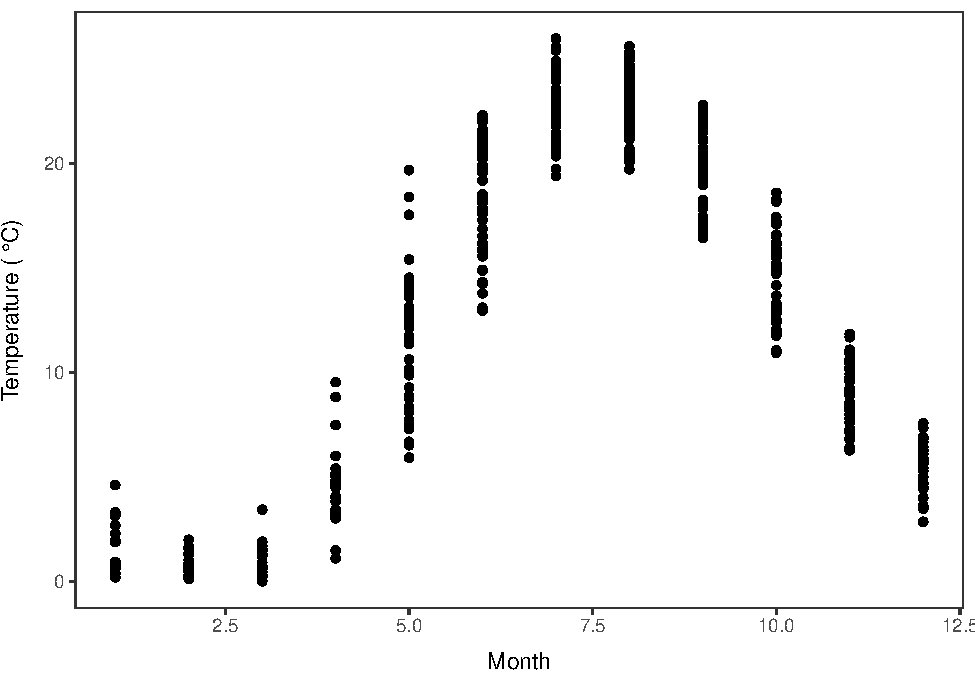
\includegraphics{worstr_files/figure-latex/unnamed-chunk-105-1.pdf}

Okay, now we need to fix that pesky x-axis scale to use whole months or text labels.

To fix the axis scales, we've actually got to do a little bit of work this time. In this case the easiest thing to do is probably to make a categorical variable out of the column \texttt{month}, which is an integer. We can do this using some fancy indexing with the built-in object that contains month abbreviations, \texttt{month.abb} in base R.

\begin{Shaded}
\begin{Highlighting}[]
\NormalTok{surface}\OperatorTok{$}\NormalTok{c_month <-}\StringTok{ }\KeywordTok{factor}\NormalTok{(month.abb[surface}\OperatorTok{$}\NormalTok{month], }\DataTypeTok{levels=}\NormalTok{month.abb)}
\end{Highlighting}
\end{Shaded}

Whoa, that was a heavy lift (sarcasm). Let's see how that changes the appearance of our plot:

\begin{Shaded}
\begin{Highlighting}[]
\NormalTok{s <-}\StringTok{ }\KeywordTok{ggplot}\NormalTok{(surface, }\KeywordTok{aes}\NormalTok{(}\DataTypeTok{x =}\NormalTok{ c_month, }\DataTypeTok{y =}\NormalTok{ temp)) }\OperatorTok{+}
\StringTok{  }\KeywordTok{geom_point}\NormalTok{() }\OperatorTok{+}\StringTok{ }
\StringTok{  }\KeywordTok{xlab}\NormalTok{(}\StringTok{"Month"}\NormalTok{) }\OperatorTok{+}
\StringTok{  }\KeywordTok{ylab}\NormalTok{(}\KeywordTok{expression}\NormalTok{(}\KeywordTok{paste}\NormalTok{(}\StringTok{"Temperature ( "}\NormalTok{, degree, }\StringTok{"C)"}\NormalTok{))) }\OperatorTok{+}
\StringTok{  }\KeywordTok{theme_bw}\NormalTok{() }\OperatorTok{+}
\StringTok{  }\KeywordTok{theme}\NormalTok{(}\DataTypeTok{axis.title.x =} \KeywordTok{element_text}\NormalTok{(}\DataTypeTok{vjust =} \DecValTok{-1}\NormalTok{),}
        \DataTypeTok{axis.title.y =} \KeywordTok{element_text}\NormalTok{(}\DataTypeTok{vjust =} \DecValTok{3}\NormalTok{),}
        \DataTypeTok{panel.grid =} \KeywordTok{element_blank}\NormalTok{()}
\NormalTok{  )}
\KeywordTok{print}\NormalTok{(s)}
\end{Highlighting}
\end{Shaded}

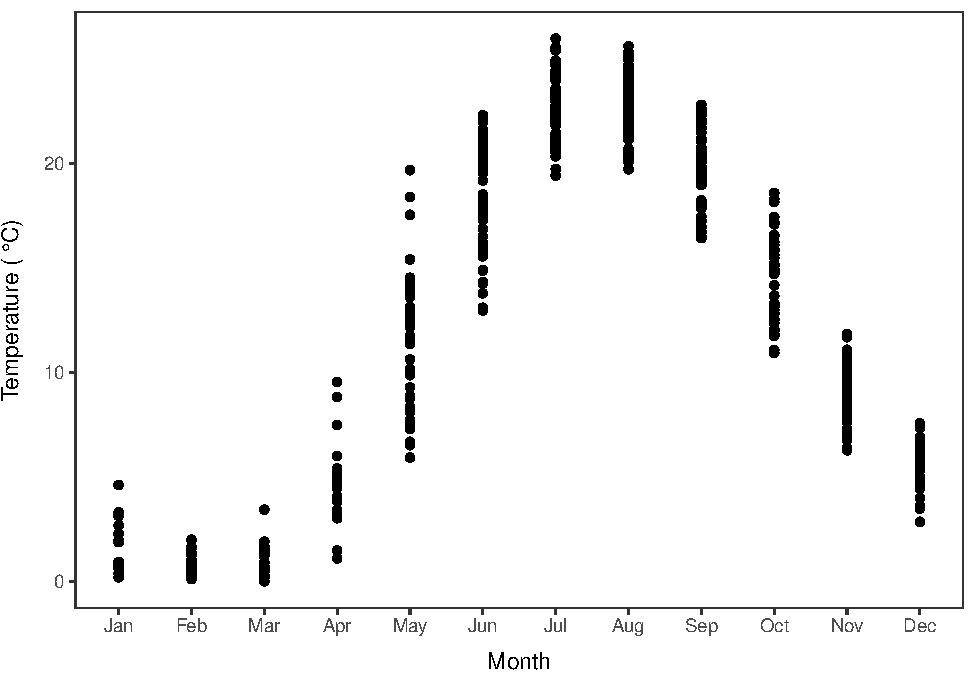
\includegraphics{worstr_files/figure-latex/unnamed-chunk-107-1.pdf}
This is starting to look really nice.

Finally, we just add a little transparency to the points by specifying \texttt{alpha\ =\ 0.2} inside of \texttt{geom\_point()} and we are good to go!

\begin{Shaded}
\begin{Highlighting}[]
\NormalTok{s <-}\StringTok{ }\KeywordTok{ggplot}\NormalTok{(surface, }\KeywordTok{aes}\NormalTok{(}\DataTypeTok{x =}\NormalTok{ c_month, }\DataTypeTok{y =}\NormalTok{ temp)) }\OperatorTok{+}
\StringTok{  }\KeywordTok{geom_point}\NormalTok{(}\DataTypeTok{alpha =} \FloatTok{0.2}\NormalTok{) }\OperatorTok{+}\StringTok{ }
\StringTok{  }\KeywordTok{xlab}\NormalTok{(}\StringTok{"Month"}\NormalTok{) }\OperatorTok{+}
\StringTok{  }\KeywordTok{ylab}\NormalTok{(}\KeywordTok{expression}\NormalTok{(}\KeywordTok{paste}\NormalTok{(}\StringTok{"Temperature ( "}\NormalTok{, degree, }\StringTok{"C)"}\NormalTok{))) }\OperatorTok{+}
\StringTok{  }\KeywordTok{theme_bw}\NormalTok{() }\OperatorTok{+}
\StringTok{  }\KeywordTok{theme}\NormalTok{(}\DataTypeTok{axis.title.x =} \KeywordTok{element_text}\NormalTok{(}\DataTypeTok{vjust =} \DecValTok{-1}\NormalTok{),}
        \DataTypeTok{axis.title.y =} \KeywordTok{element_text}\NormalTok{(}\DataTypeTok{vjust =} \DecValTok{3}\NormalTok{),}
        \DataTypeTok{panel.grid =} \KeywordTok{element_blank}\NormalTok{()}
\NormalTok{  )}
\KeywordTok{print}\NormalTok{(s)}
\end{Highlighting}
\end{Shaded}

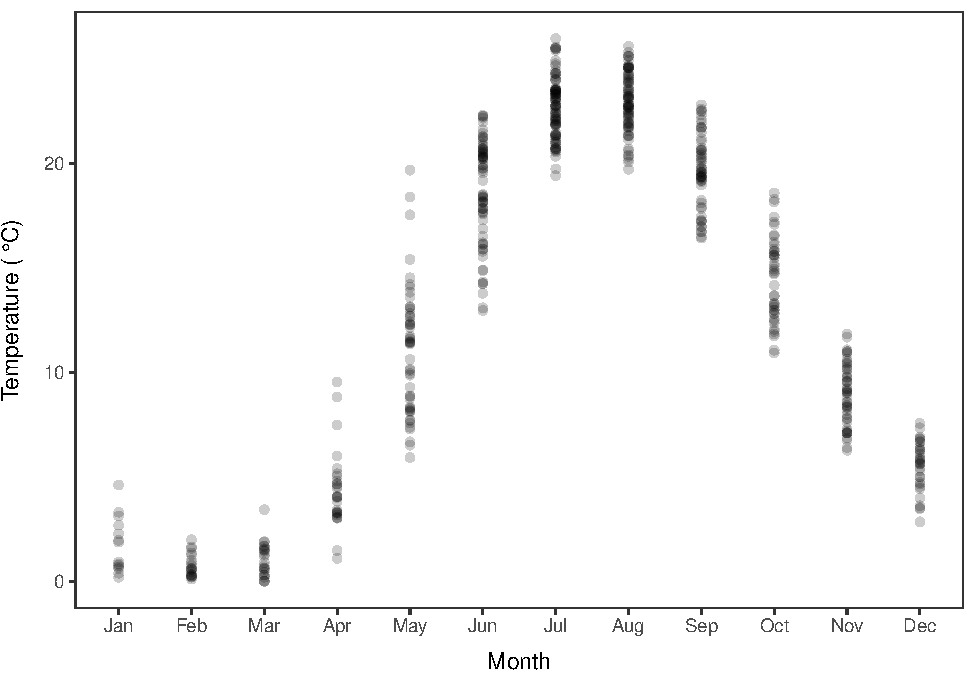
\includegraphics{worstr_files/figure-latex/unnamed-chunk-108-1.pdf}

Looks just like the one we made with base graphics!

\hypertarget{gglines}{%
\subsection{Lines}\label{gglines}}

Most of the time we plot line graphs, whether in base graphics or using \texttt{ggplot2}, we are going to be adding them to existing plots. This was really straightforward in base graphics. It is only slightly more complicated in \texttt{ggplot2}.

We'll start with the default line graph, and then add it to the scatter plot from the previous section.

Let's calculate monthly means of surface temperature in Otsego Lake again:

\begin{Shaded}
\begin{Highlighting}[]
\NormalTok{mids <-}\StringTok{ }\NormalTok{surface }\OperatorTok
\StringTok{  }\KeywordTok{group_by}\NormalTok{(month) }\OperatorTok
\StringTok{  }\KeywordTok{summarize}\NormalTok{(}\DataTypeTok{avg =} \KeywordTok{mean}\NormalTok{(temp))}
\end{Highlighting}
\end{Shaded}

Now plot it with \texttt{ggplot()}:

\begin{Shaded}
\begin{Highlighting}[]
\NormalTok{lp <-}\StringTok{ }\KeywordTok{ggplot}\NormalTok{(mids, }\KeywordTok{aes}\NormalTok{(}\DataTypeTok{x =}\NormalTok{ month, }\DataTypeTok{y =}\NormalTok{ avg)) }\OperatorTok{+}
\StringTok{  }\KeywordTok{geom_line}\NormalTok{()}

\KeywordTok{print}\NormalTok{(lp)}
\end{Highlighting}
\end{Shaded}

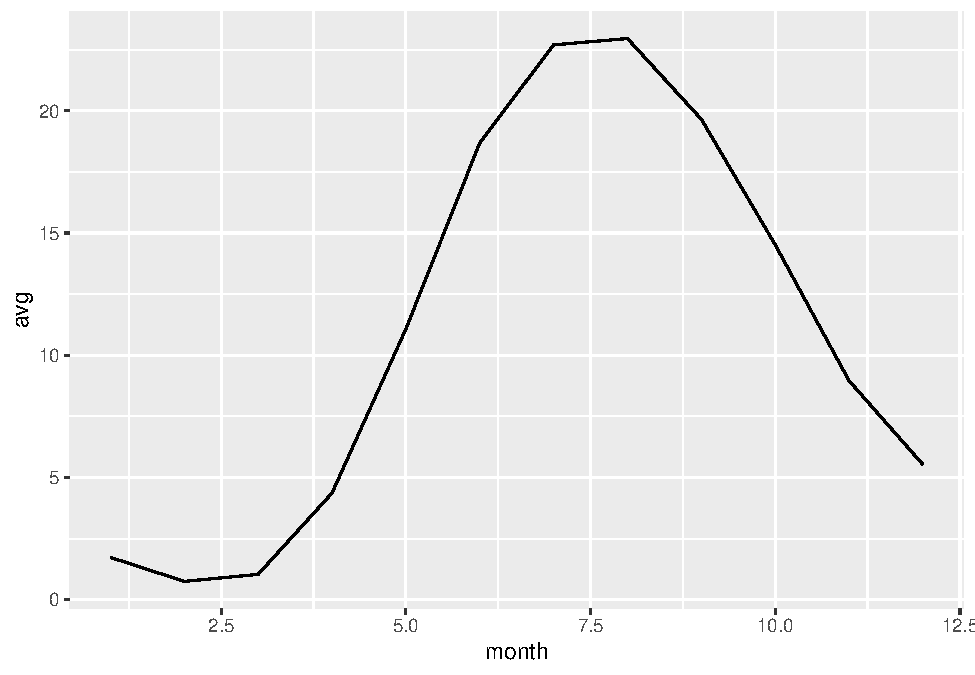
\includegraphics{worstr_files/figure-latex/unnamed-chunk-110-1.pdf}

There you have it!

Now, we just need to add this to our scatterplot that we made previously. To do this, we have to insert \texttt{geom\_line()} in the code, but we must specify

\begin{Shaded}
\begin{Highlighting}[]
\NormalTok{s <-}\StringTok{ }\KeywordTok{ggplot}\NormalTok{(}\DataTypeTok{data =}\NormalTok{ surface, }\DataTypeTok{mapping =} \KeywordTok{aes}\NormalTok{(}\DataTypeTok{x =}\NormalTok{ c_month, }\DataTypeTok{y =}\NormalTok{ temp)) }\OperatorTok{+}
\StringTok{  }\KeywordTok{geom_point}\NormalTok{(}\DataTypeTok{alpha =} \FloatTok{0.20}\NormalTok{) }\OperatorTok{+}\StringTok{ }
\StringTok{  }\KeywordTok{geom_line}\NormalTok{(}\DataTypeTok{mapping =} \KeywordTok{aes}\NormalTok{(}\DataTypeTok{x =}\NormalTok{ month, }\DataTypeTok{y =}\NormalTok{ avg),}
            \DataTypeTok{data =}\NormalTok{ mids,}
            \DataTypeTok{color =} \StringTok{'gray40'}\NormalTok{,}
            \DataTypeTok{lty =} \DecValTok{3}\NormalTok{,}
            \DataTypeTok{lwd =} \DecValTok{1}\NormalTok{) }\OperatorTok{+}
\StringTok{  }\KeywordTok{xlab}\NormalTok{(}\StringTok{"Month"}\NormalTok{) }\OperatorTok{+}
\StringTok{  }\KeywordTok{ylab}\NormalTok{(}\KeywordTok{expression}\NormalTok{(}\KeywordTok{paste}\NormalTok{(}\StringTok{"Temperature ( "}\NormalTok{, degree, }\StringTok{"C)"}\NormalTok{))) }\OperatorTok{+}
\StringTok{  }\KeywordTok{theme_bw}\NormalTok{() }\OperatorTok{+}
\StringTok{  }\KeywordTok{theme}\NormalTok{(}\DataTypeTok{axis.title.x =} \KeywordTok{element_text}\NormalTok{(}\DataTypeTok{vjust =} \DecValTok{-1}\NormalTok{),}
        \DataTypeTok{axis.title.y =} \KeywordTok{element_text}\NormalTok{(}\DataTypeTok{vjust =} \DecValTok{3}\NormalTok{),}
        \DataTypeTok{panel.grid =} \KeywordTok{element_blank}\NormalTok{()}
\NormalTok{  )}

\KeywordTok{print}\NormalTok{(s)}
\end{Highlighting}
\end{Shaded}

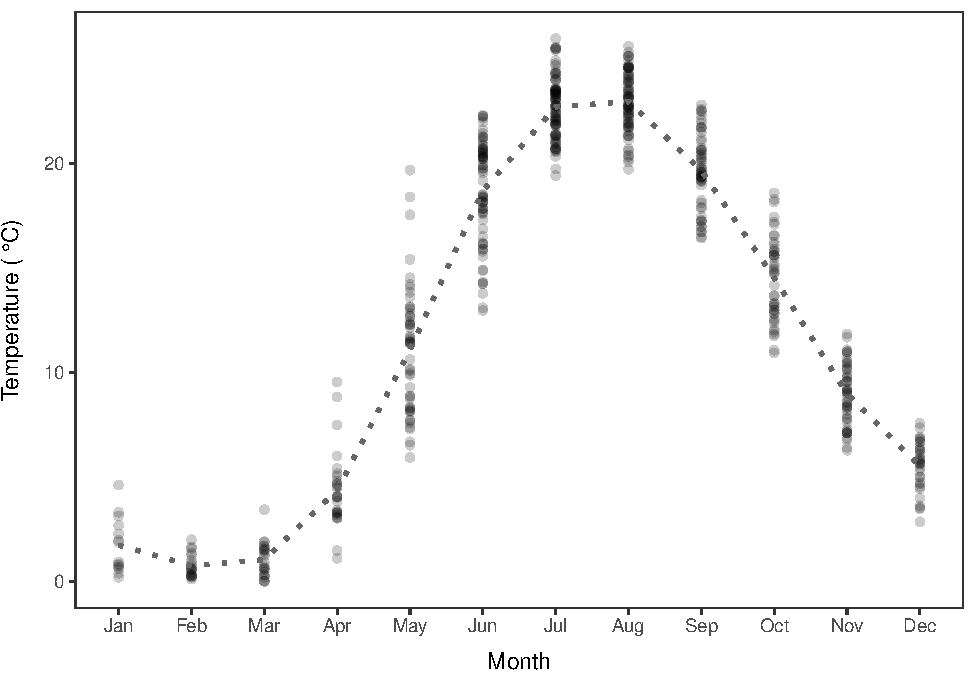
\includegraphics{worstr_files/figure-latex/unnamed-chunk-111-1.pdf}

We will continue to use this approach throughout the book to plot raw data and model predictions. So, if it is giving you trouble now, spend some extra time with it.

\hypertarget{ggboxplots}{%
\subsection{Boxplots and}\label{ggboxplots}}

To wrap up our tour of plotting examples in \texttt{ggplot2}, we will reproduce (more or less) the box plots we made in \protect\hyperlink{boxplots}{base graphics}.

Make the default box plot of surface water temperatures in Otsego Lake, NY. Notice that we use the \texttt{c\_month} variable that we made previously in the \texttt{surface} data so R knows these are groups.

\begin{Shaded}
\begin{Highlighting}[]
\NormalTok{bp <-}\StringTok{ }\KeywordTok{ggplot}\NormalTok{(surface, }\KeywordTok{aes}\NormalTok{(}\DataTypeTok{x =}\NormalTok{ c_month, }\DataTypeTok{y =}\NormalTok{ temp)) }\OperatorTok{+}\StringTok{ }\KeywordTok{geom_boxplot}\NormalTok{()}

\KeywordTok{print}\NormalTok{(bp)}
\end{Highlighting}
\end{Shaded}

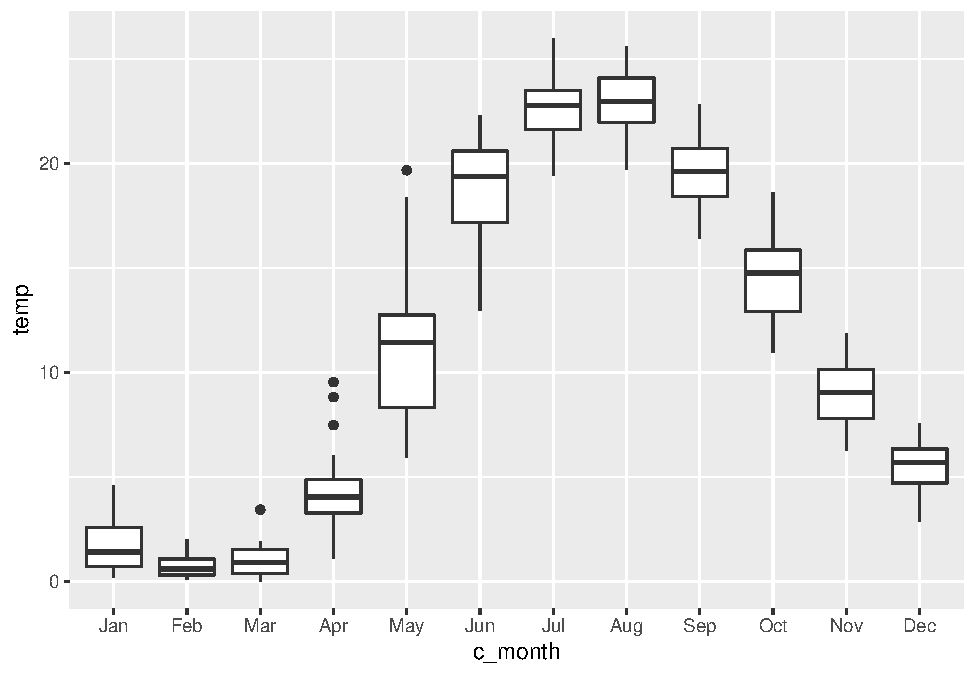
\includegraphics{worstr_files/figure-latex/unnamed-chunk-112-1.pdf}

If we add changes we made to previous plots here, then we can get a cleaner look:

\begin{Shaded}
\begin{Highlighting}[]
\NormalTok{bp <-}\StringTok{ }\KeywordTok{ggplot}\NormalTok{(surface, }\KeywordTok{aes}\NormalTok{(}\DataTypeTok{x =}\NormalTok{ c_month, }\DataTypeTok{y =}\NormalTok{ temp)) }\OperatorTok{+}
\StringTok{  }\KeywordTok{geom_boxplot}\NormalTok{(}\DataTypeTok{color =} \StringTok{'gray40'}\NormalTok{, }\DataTypeTok{fill =} \StringTok{'gray87'}\NormalTok{, }\DataTypeTok{width =} \FloatTok{0.3}\NormalTok{) }\OperatorTok{+}
\StringTok{  }\KeywordTok{xlab}\NormalTok{(}\StringTok{"Month"}\NormalTok{) }\OperatorTok{+}
\StringTok{  }\KeywordTok{ylab}\NormalTok{(}\KeywordTok{expression}\NormalTok{(}\KeywordTok{paste}\NormalTok{(}\StringTok{"Temperature ( "}\NormalTok{, degree, }\StringTok{"C)"}\NormalTok{))) }\OperatorTok{+}
\StringTok{  }\KeywordTok{theme_bw}\NormalTok{() }\OperatorTok{+}
\StringTok{  }\KeywordTok{theme}\NormalTok{(}\DataTypeTok{axis.title.x =} \KeywordTok{element_text}\NormalTok{(}\DataTypeTok{vjust =} \DecValTok{-1}\NormalTok{),}
        \DataTypeTok{axis.title.y =} \KeywordTok{element_text}\NormalTok{(}\DataTypeTok{vjust =} \DecValTok{3}\NormalTok{),}
        \DataTypeTok{panel.grid =} \KeywordTok{element_blank}\NormalTok{()}
\NormalTok{  )}

\KeywordTok{print}\NormalTok{(bp)}
\end{Highlighting}
\end{Shaded}

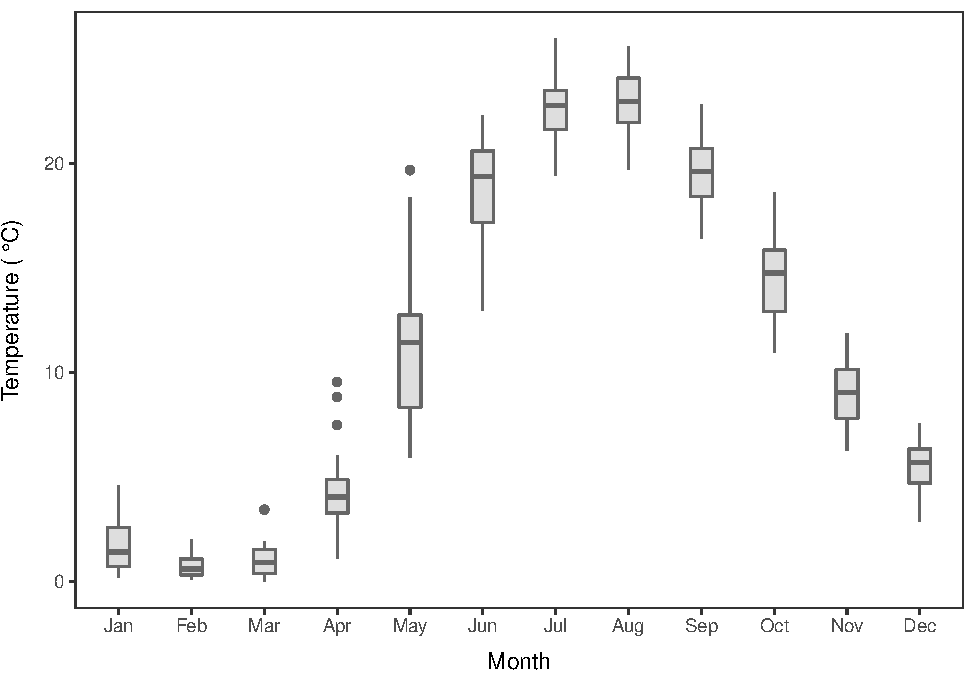
\includegraphics{worstr_files/figure-latex/unnamed-chunk-113-1.pdf}

And, of course, we can add our ``jittered'', raw data points over the top to show the spread.

\begin{Shaded}
\begin{Highlighting}[]
\NormalTok{bp <-}\StringTok{ }\KeywordTok{ggplot}\NormalTok{(surface, }\KeywordTok{aes}\NormalTok{(}\DataTypeTok{x =}\NormalTok{ c_month, }\DataTypeTok{y =}\NormalTok{ temp)) }\OperatorTok{+}
\StringTok{  }\KeywordTok{geom_boxplot}\NormalTok{(}\DataTypeTok{color =} \StringTok{'gray40'}\NormalTok{, }\DataTypeTok{fill =} \StringTok{'gray87'}\NormalTok{, }\DataTypeTok{width =} \FloatTok{0.4}\NormalTok{) }\OperatorTok{+}
\StringTok{  }\KeywordTok{geom_jitter}\NormalTok{(}\DataTypeTok{size =} \FloatTok{.5}\NormalTok{, }\DataTypeTok{width =} \FloatTok{0.1}\NormalTok{) }\OperatorTok{+}
\StringTok{  }\KeywordTok{xlab}\NormalTok{(}\StringTok{"Month"}\NormalTok{) }\OperatorTok{+}
\StringTok{  }\KeywordTok{ylab}\NormalTok{(}\KeywordTok{expression}\NormalTok{(}\KeywordTok{paste}\NormalTok{(}\StringTok{"Temperature ( "}\NormalTok{, degree, }\StringTok{"C)"}\NormalTok{))) }\OperatorTok{+}
\StringTok{  }\KeywordTok{theme_bw}\NormalTok{() }\OperatorTok{+}
\StringTok{  }\KeywordTok{theme}\NormalTok{(}\DataTypeTok{axis.title.x =} \KeywordTok{element_text}\NormalTok{(}\DataTypeTok{vjust =} \DecValTok{-1}\NormalTok{),}
        \DataTypeTok{axis.title.y =} \KeywordTok{element_text}\NormalTok{(}\DataTypeTok{vjust =} \DecValTok{3}\NormalTok{),}
        \DataTypeTok{panel.grid =} \KeywordTok{element_blank}\NormalTok{()}
\NormalTok{  )}

\KeywordTok{print}\NormalTok{(bp)}
\end{Highlighting}
\end{Shaded}

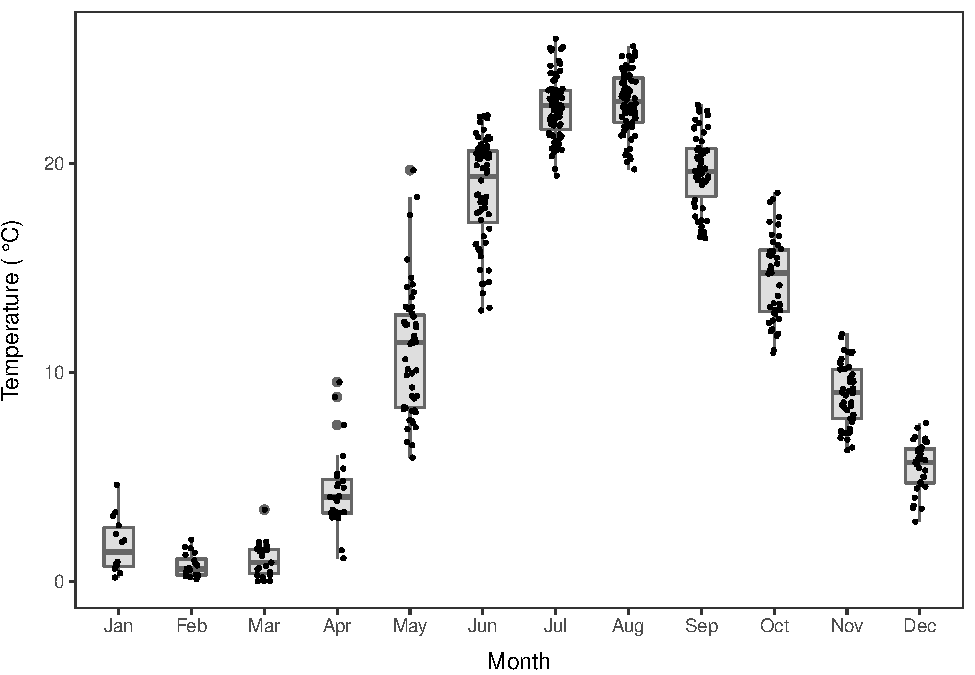
\includegraphics{worstr_files/figure-latex/unnamed-chunk-114-1.pdf}

\hypertarget{next4}{%
\section{Next steps}\label{next4}}

Hopefully this chapter provided you with a basic overview of plotting in R. If you struggled with these exercises, practice them again, or check out some \href{https://danstich.github.io/stich/classes/BIOL217/resources.html}{additional online resources}. In the coming chapters, we will continue to add functionality and complexity to how we use these kinds of plots. We'll look at how to compare two groups within a single plot in \protect\hyperlink{Chapter6}{Chapter 6} when we dive into sampling distributions. And, eventually we will learn how to plot predictions from our statistical model against observed data from Chapter 8 onward.

\hypertarget{sampling-distributions-in-r}{%
\chapter{Sampling distributions in R}\label{sampling-distributions-in-r}}

If we can describe the shape of a probability distribution for a random variable like temperature we can make predictions about the world. Sinister? Maybe. These are temperatures that I simulated from the Hudson River using historical data to estimate parameters of a multivariate normal distribution (muwahahaha).

In this Chapter, we'll talk about probability and probability distributions as a backdrop for the models that we will be working with during the next several chapters. When we describe these from data we have collected, we call them \textbf{sampling distributions}. Probability theory is central to statistical techniques, so it will be important for you to have a pretty firm understanding of this to grab hold of big ideas later on. For now, play along and try to understand how they work. We'll swing back later for a refresher.

In order to complete this Chapter, you will need to have the \texttt{ggplot2}, \texttt{MASS}, and \texttt{Rlab} packages loaded. The only one you should need to install is the \texttt{Rlab} package because \texttt{MASS} is installed when you install R, and we already installed \texttt{ggplot2} with the \texttt{tidyverse} in \protect\hyperlink{Chapter3}{Chapter3}.

I'm going to load these now. In general, it is good practice to put these at the top of the script so we know they are needed.

\begin{Shaded}
\begin{Highlighting}[]
\KeywordTok{library}\NormalTok{(ggplot2)}
\KeywordTok{library}\NormalTok{(MASS)}
\KeywordTok{library}\NormalTok{(Rlab)}
\end{Highlighting}
\end{Shaded}

None of the class data are required to complete this chapter.

\hypertarget{what-are-sampling-distributions}{%
\section{What are sampling distributions?}\label{what-are-sampling-distributions}}

When we talk about sampling distributions, we are talking about the probability that a variable we can measure (e.g.~temperature) takes on some value. In most cases, there is a higher probability that the variable will take on certain values than others. That probability may be governed by any number of processes and thus may assume a number of different shapes with respect to the likelihood of any given value of our variable. The differences in the shapes that we assume, and the mathematical parameters that we use to describe those shapes are called ``probability distributions''. And, when they are estimated from data, they are sampling distributions.

There was a time when biologists were largely restricted to using models that relied heavily on the assumption that the things we measured, and their errors, followed ``normal'' distributions, which you have probably heard of or seen in a scientific paper. This was because of how computationally intensive other methods were. This often led to the use of strictly parametric tools like ANOVA and t-tests, or the use of strictly non-parametric tools like frequency analyses and rank-order methods. While these are still useful techniques in our toolboxes, that time has passed, and now we have access to a wide range of tools that allow us to extend simple parametric and non-parametric tools to relax or change distributional assumptions. We will discuss these throughout the book, but we need to look at the underlying distributions that govern our decisions about which of these tools to use. So, this week we'll look at a few probability distributions that correspond to sampling distributions we frequently encounter in biology. To wrap-up, we will use this new information to talk about how we calculate descriptive statistics such as means and standard deviations from samples.

\hypertarget{probability-distributions-in-r}{%
\section{Probability distributions in R}\label{probability-distributions-in-r}}

R has a number of built-in distribution types, and there are random-number generators associated with most or all of these that will allow us to take random samples from a distribution (like picking numbers out of a hat!). This is useful for data simulation, but is also helpful for us to learn about probability distributions and how their parameters affect the shape, spread, scale, location, etc. of those distributions. We will briefly discuss concepts like skew because of how they can help us think about the assumptions that we are making (or breaking!) in the models that we use.

For this class, we will focus on one major family of distributions and then zero in on a few distributions within this family that you are guaranteed to encounter throughout your career.

\hypertarget{exponential-family}{%
\section{Exponential family}\label{exponential-family}}

Most or all of the distributions we will use for this class come from the \textbf{exponential family} of distributions.

The exponential family is very flexible, and whether you know it or not, it includes most of the distributions one might use to describe every day phenomena. It includes most of the probability distributions with which you are familiar, and many more. Just ask this \emph{very} reliable \href{https://en.wikipedia.org/wiki/Exponential_family}{Wikipedia entry}. Oh, let's face it, you were going there anyway, I just cut out the Google step.

Take a look at the table at the bottom of this Wikipedia page just to get an idea of how many distributions are included within the exponential! Holy cow! We're not going to look at all of these in this class- I just want you to be aware that this is a \textbf{huge} family of specific distributions.

\textbf{Distributions that we'll focus on in this chapter}:

\textbf{1. Continuous distributions}
Normal (Gaussian)
Lognormal
Beta
Uniform
\textbf{2. Discrete distributions}
Bernouli
Binomial
Multinomial
Poisson
Negative binomial

\hypertarget{continuous-distributions}{%
\section{Continuous distributions}\label{continuous-distributions}}

The normal distribution

This is one distribution with which most of you have at least some nodding acquaintance. It is the classic ``bell curve'' that college students once dreaded in upper-level courses. I don't know if it's a thing anymore. Go Google it.

The \textbf{normal distribution} is defined by two parameters:

\begin{enumerate}
\def\labelenumi{\arabic{enumi}.}
\item
  The mean (\(\mu\))
\item
  The variance (\(\sigma^2\))
\end{enumerate}

Let's take a look at what the normal distribution looks like. We'll start with a special one called the standard normal (or \emph{z}) distribution. The standard normal is a normal distribution with a mean of zero and a variance of 1. This one is really cool because the standard deviation (\(\sigma\)) is the square-root of the variance, and in this special case \(\sqrt{1} = 1\), so the variance and standard deviation are equal! And because of this property, and other normal distribution can be converted to a standard normal using z-standardization, which we'll talk about later. How exciting is that?

First, take a sample from a normal distribution:

\begin{Shaded}
\begin{Highlighting}[]
\NormalTok{samp <-}\StringTok{ }\KeywordTok{rnorm}\NormalTok{(}\DataTypeTok{n =} \DecValTok{10000}\NormalTok{, }\DataTypeTok{mean =} \DecValTok{0}\NormalTok{, }\DataTypeTok{sd =} \DecValTok{1}\NormalTok{)}
\end{Highlighting}
\end{Shaded}

Now, plot a histogram using the sick new skills you got in \protect\hyperlink{Chapter4}{Chapter 4}

\begin{Shaded}
\begin{Highlighting}[]
\NormalTok{p <-}\StringTok{ }\KeywordTok{ggplot}\NormalTok{() }\OperatorTok{+}\StringTok{ }
\StringTok{  }\KeywordTok{geom_histogram}\NormalTok{(}\KeywordTok{aes}\NormalTok{(samp), }\DataTypeTok{binwidth =} \DecValTok{1}\NormalTok{) }\OperatorTok{+}\StringTok{ }
\StringTok{  }\KeywordTok{scale_x_continuous}\NormalTok{(}\DataTypeTok{limits=}\KeywordTok{c}\NormalTok{(}\OperatorTok{-}\DecValTok{7}\NormalTok{,}\DecValTok{7}\NormalTok{), }\DataTypeTok{expand =} \KeywordTok{c}\NormalTok{(}\DecValTok{0}\NormalTok{, }\DecValTok{0}\NormalTok{)) }\OperatorTok{+}\StringTok{ }
\StringTok{  }\KeywordTok{scale_y_continuous}\NormalTok{(}\DataTypeTok{expand =} \KeywordTok{c}\NormalTok{(}\DecValTok{0}\NormalTok{, }\DecValTok{1}\NormalTok{)) }\OperatorTok{+}\StringTok{ }
\StringTok{  }\KeywordTok{xlab}\NormalTok{(}\StringTok{"Value"}\NormalTok{) }\OperatorTok{+}
\StringTok{  }\KeywordTok{ylab}\NormalTok{(}\StringTok{"Count"}\NormalTok{) }\OperatorTok{+}
\StringTok{  }\KeywordTok{theme_classic}\NormalTok{() }\OperatorTok{+}
\StringTok{  }\KeywordTok{theme}\NormalTok{(}
    \DataTypeTok{axis.title.x =} \KeywordTok{element_text}\NormalTok{(}\DataTypeTok{vjust =} \DecValTok{-1}\NormalTok{),}
    \DataTypeTok{axis.title.y =} \KeywordTok{element_text}\NormalTok{(}\DataTypeTok{vjust =} \DecValTok{3}\NormalTok{),}
    \DataTypeTok{panel.grid =} \KeywordTok{element_blank}\NormalTok{()}
\NormalTok{  )}
\KeywordTok{print}\NormalTok{(p)}
\end{Highlighting}
\end{Shaded}

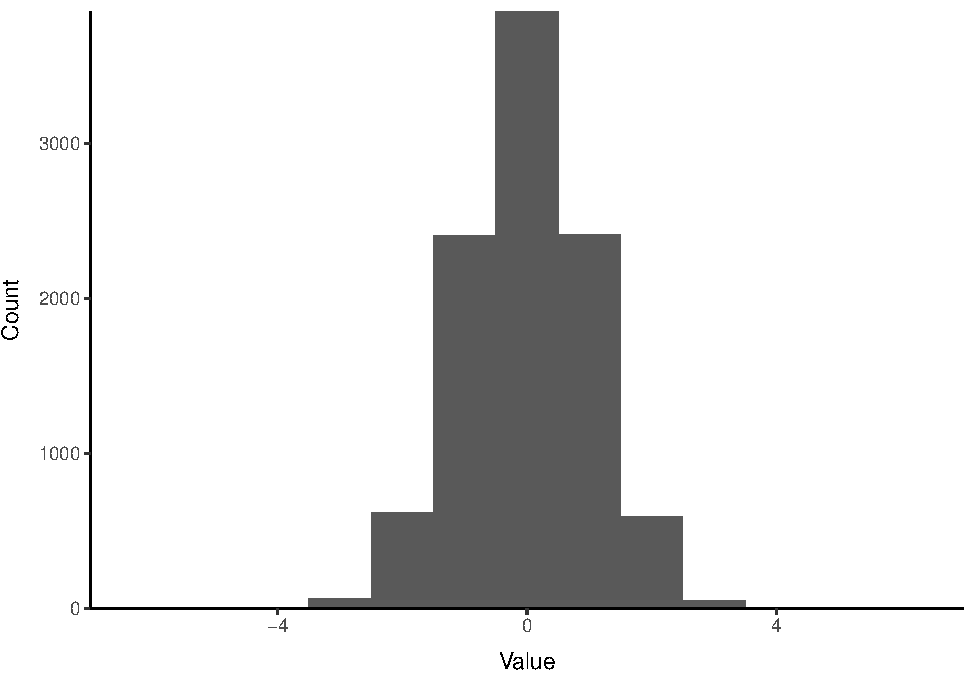
\includegraphics{worstr_files/figure-latex/unnamed-chunk-117-1.pdf}

Pretty!

Because this sample is from a \textbf{continuous} distribution, we might actually wish to represent this distribution with a probability density function. You can think of this as R calculating the relative probability of an given value. It implies a continuous surface, rather than the discrete bins like the histogram. In reality it doesn't matter because at best we chop continuous distributions into tiny little bins when we do things like integrals, and R bases \texttt{binwidth} in histograms off a density function anyway (aaaaah!).

Density plots are a new one for us, so let's try them out. If you scroll back and forth, you'll notice that the code below is basically identical to the histogram above except for labels and scales. We just replaced the histogram geometry (\texttt{geom\_histogram}) with a density-based geometry (\texttt{geom\_density}). Here, we use \texttt{fill\ =\ 1} to trick R into filling the area under the line because we have no grouping variables. By default, this is interpreted as \texttt{\textquotesingle{}black\textquotesingle{}}, so we add an alpha channel for transparency.

\begin{Shaded}
\begin{Highlighting}[]
\NormalTok{p <-}\StringTok{ }\KeywordTok{ggplot}\NormalTok{() }\OperatorTok{+}\StringTok{ }
\StringTok{  }\KeywordTok{geom_density}\NormalTok{(}\KeywordTok{aes}\NormalTok{(samp), }\DataTypeTok{alpha =} \FloatTok{.1}\NormalTok{, }\DataTypeTok{fill =} \DecValTok{1}\NormalTok{) }\OperatorTok{+}\StringTok{ }
\StringTok{  }\KeywordTok{scale_x_continuous}\NormalTok{(}\DataTypeTok{limits =} \KeywordTok{c}\NormalTok{(}\OperatorTok{-}\DecValTok{7}\NormalTok{,}\DecValTok{7}\NormalTok{), }\DataTypeTok{expand =} \KeywordTok{c}\NormalTok{(}\DecValTok{0}\NormalTok{, }\DecValTok{0}\NormalTok{)) }\OperatorTok{+}\StringTok{ }
\StringTok{  }\KeywordTok{scale_y_continuous}\NormalTok{(}\DataTypeTok{expand =} \KeywordTok{c}\NormalTok{(}\DecValTok{0}\NormalTok{, }\DecValTok{0}\NormalTok{)) }\OperatorTok{+}\StringTok{ }
\StringTok{  }\KeywordTok{xlab}\NormalTok{(}\StringTok{"Value"}\NormalTok{) }\OperatorTok{+}
\StringTok{  }\KeywordTok{ylab}\NormalTok{(}\StringTok{"Density"}\NormalTok{) }\OperatorTok{+}
\StringTok{  }\KeywordTok{theme_classic}\NormalTok{() }\OperatorTok{+}
\StringTok{  }\KeywordTok{theme}\NormalTok{(}
    \DataTypeTok{axis.title.x =} \KeywordTok{element_text}\NormalTok{(}\DataTypeTok{vjust =} \DecValTok{-1}\NormalTok{),}
    \DataTypeTok{axis.title.y =} \KeywordTok{element_text}\NormalTok{(}\DataTypeTok{vjust =} \DecValTok{3}\NormalTok{),}
    \DataTypeTok{panel.grid =} \KeywordTok{element_blank}\NormalTok{()}
\NormalTok{  )}
\KeywordTok{print}\NormalTok{(p)}
\end{Highlighting}
\end{Shaded}

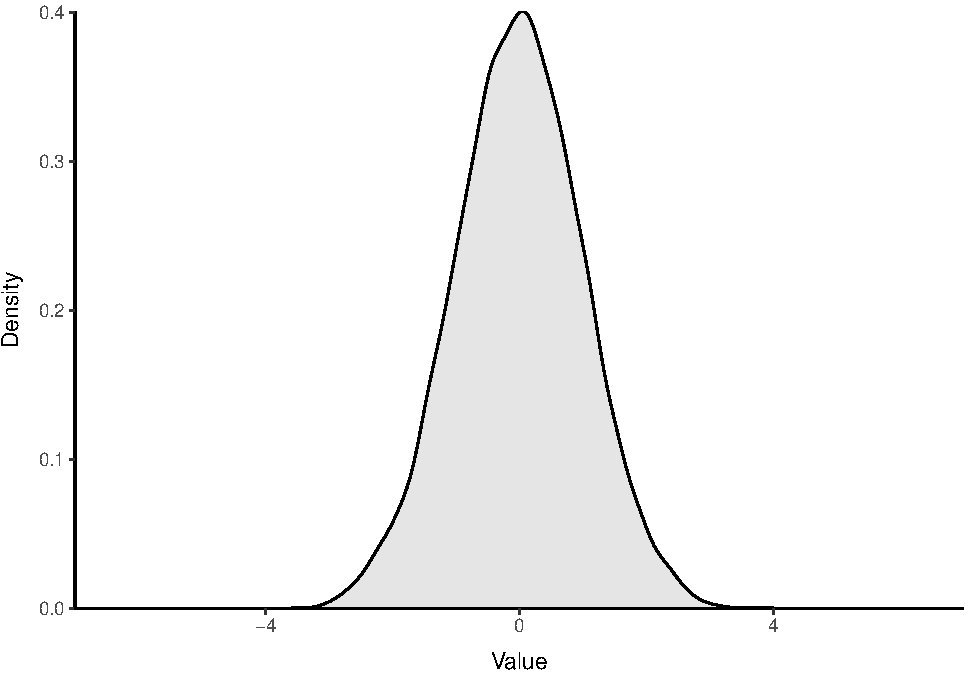
\includegraphics{worstr_files/figure-latex/unnamed-chunk-118-1.pdf}

Excellent use of \texttt{ggplot()} to make a figure that looks like the clunky base graphics. Maybe you can improve on it in the homework assignment?

We can change the parameters of the standard normal to change both the location and the scale of our distribution. The influence of changing the mean, or average, on the location of a distribution is perhaps obvious. But, the influence of variance may be less intuitive, so let's have a look!

Create two more random samples, one with a larger \texttt{sd} and one with a smaller \texttt{sd}, to see how this changes the shape of the distribution:

\begin{Shaded}
\begin{Highlighting}[]
\NormalTok{samp2 <-}\StringTok{ }\KeywordTok{rnorm}\NormalTok{(}\DataTypeTok{n =} \FloatTok{1e4}\NormalTok{, }\DataTypeTok{mean =} \DecValTok{0}\NormalTok{, }\DataTypeTok{sd =} \DecValTok{2}\NormalTok{)}
\NormalTok{samp3 <-}\StringTok{ }\KeywordTok{rnorm}\NormalTok{(}\DataTypeTok{n =} \FloatTok{1e4}\NormalTok{, }\DataTypeTok{mean =} \DecValTok{0}\NormalTok{, }\DataTypeTok{sd =} \FloatTok{.5}\NormalTok{)}
\end{Highlighting}
\end{Shaded}

Let's put them in a data frame with \texttt{samp} so they're easy to plot. We combine all three random samples into one column called \texttt{Value}. Then, we create a column to hold the standard deviation used in each sample (\texttt{Sigma}). If we make that one into a factor, we can use the \texttt{Sigma} columns to plot the samples as separate lines by tweaking our plotting code.

\begin{Shaded}
\begin{Highlighting}[]
\NormalTok{normals <-}\StringTok{ }\KeywordTok{data.frame}\NormalTok{(}
  \DataTypeTok{Value =} \KeywordTok{c}\NormalTok{(samp, samp2, samp3),}
  \DataTypeTok{Sigma =} \KeywordTok{factor}\NormalTok{(}
    \KeywordTok{c}\NormalTok{(}
      \KeywordTok{rep}\NormalTok{(}\DecValTok{1}\NormalTok{, }\KeywordTok{length}\NormalTok{(samp)), }
      \KeywordTok{rep}\NormalTok{(}\DecValTok{2}\NormalTok{, }\KeywordTok{length}\NormalTok{(samp2)), }
      \KeywordTok{rep}\NormalTok{(.}\DecValTok{5}\NormalTok{, }\KeywordTok{length}\NormalTok{(samp3))}
\NormalTok{    )}
\NormalTok{  )}
\NormalTok{)}
\end{Highlighting}
\end{Shaded}

Next, we can just add these to the plot to compare the sampling distributions. This time, we tell R to fill the area under our lines based on sample ID with a default color scheme by saying \texttt{fill\ =\ Sigma} in our \texttt{ggplot()} call. We also added \texttt{color\ =\ Sigma} to make the lines the same default colors. Remember, you can specify your own.

\begin{Shaded}
\begin{Highlighting}[]
\NormalTok{p <-}\StringTok{ }\KeywordTok{ggplot}\NormalTok{(}\DataTypeTok{data =}\NormalTok{ normals, }
            \KeywordTok{aes}\NormalTok{(}\DataTypeTok{x =}\NormalTok{ Value, }\DataTypeTok{group =}\NormalTok{ Sigma, }\DataTypeTok{fill =}\NormalTok{ Sigma, }\DataTypeTok{color =}\NormalTok{ Sigma)) }\OperatorTok{+}
\StringTok{  }\KeywordTok{geom_density}\NormalTok{(}\DataTypeTok{adjust =} \FloatTok{1.5}\NormalTok{, }\DataTypeTok{alpha =} \FloatTok{.4}\NormalTok{) }\OperatorTok{+}
\StringTok{  }\KeywordTok{scale_x_continuous}\NormalTok{(}\DataTypeTok{limits =} \KeywordTok{c}\NormalTok{(}\OperatorTok{-}\DecValTok{7}\NormalTok{, }\DecValTok{7}\NormalTok{), }\DataTypeTok{expand =} \KeywordTok{c}\NormalTok{(}\DecValTok{0}\NormalTok{, }\DecValTok{0}\NormalTok{)) }\OperatorTok{+}\StringTok{ }
\StringTok{  }\KeywordTok{scale_y_continuous}\NormalTok{(}\DataTypeTok{expand =} \KeywordTok{c}\NormalTok{(}\DecValTok{0}\NormalTok{, }\DecValTok{0}\NormalTok{)) }\OperatorTok{+}\StringTok{ }
\StringTok{  }\KeywordTok{xlab}\NormalTok{(}\StringTok{"Value"}\NormalTok{) }\OperatorTok{+}
\StringTok{  }\KeywordTok{ylab}\NormalTok{(}\StringTok{"Density"}\NormalTok{) }\OperatorTok{+}
\StringTok{  }\KeywordTok{theme_classic}\NormalTok{() }\OperatorTok{+}
\StringTok{  }\KeywordTok{theme}\NormalTok{(}
    \DataTypeTok{axis.title.x =} \KeywordTok{element_text}\NormalTok{(}\DataTypeTok{vjust =} \DecValTok{-1}\NormalTok{),}
    \DataTypeTok{axis.title.y =} \KeywordTok{element_text}\NormalTok{(}\DataTypeTok{vjust =} \DecValTok{3}\NormalTok{),}
    \DataTypeTok{panel.grid =} \KeywordTok{element_blank}\NormalTok{()}
\NormalTok{  )}
\KeywordTok{print}\NormalTok{(p)}
\end{Highlighting}
\end{Shaded}

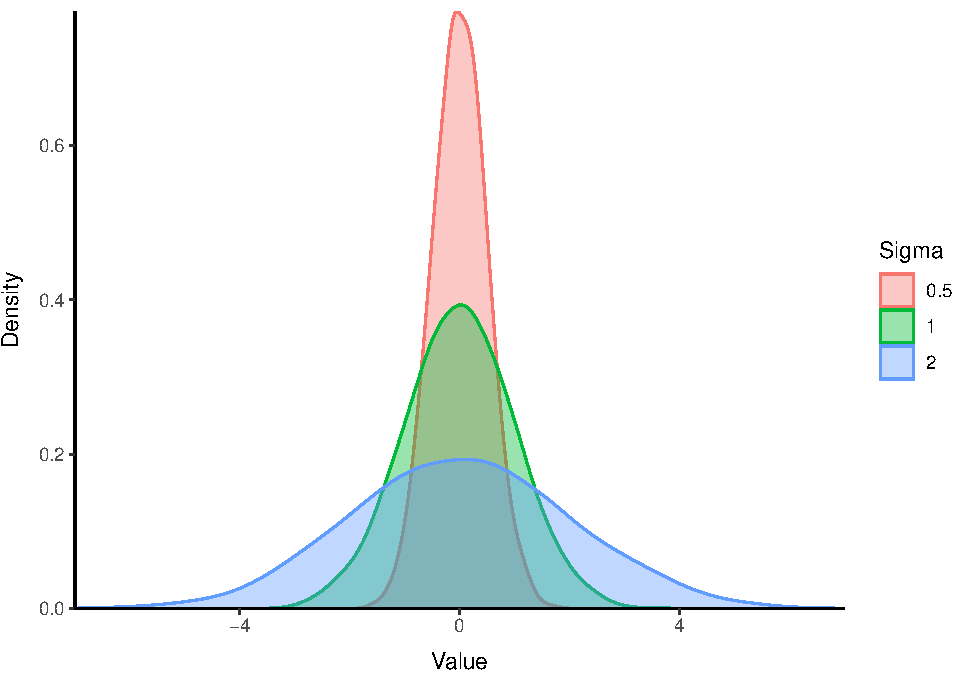
\includegraphics{worstr_files/figure-latex/unnamed-chunk-121-1.pdf}

The blue polygon in the plot above shows a distribution with greater variance than our z distribution (green). The red polygon shows a distribution with a smaller variance. Hopefully this helps demonstrate how variance influences the scale of the distribution.

\hypertarget{the-lognormal-distribution}{%
\subsection{The lognormal distribution}\label{the-lognormal-distribution}}

The \textbf{lognormal distribution} is a probability distribution that assumes our random variable is normally distributed on the \textbf{log scale}. This assumption allows us to incorporate \textbf{skew} into the normal distribution and change the location and scale of the normal distribution by transforming the parameters (\(\mu\) and \(\sigma\)) onto the log scale. This is one of the more common data transformations that you will run into, e.g.: ``We log-transformed the data to achieve normality\ldots{}''. One of the other reasons for that is that all values (positive or negative) transformed from the log to the real scale are positive, so it helps prevent us from making negative predictions about phenomena or variables that can't be less than zero.

Let's take a look at how changes to the mean change the location of this distribution:

\begin{Shaded}
\begin{Highlighting}[]
\CommentTok{# Create random samples from log-normal}
\CommentTok{# distributions with different means}
\NormalTok{samp1 <-}\StringTok{ }\KeywordTok{rlnorm}\NormalTok{(}\DataTypeTok{n=}\FloatTok{1e4}\NormalTok{, }\DataTypeTok{mean=}\DecValTok{0}\NormalTok{, }\DataTypeTok{sd=}\DecValTok{1}\NormalTok{)}
\NormalTok{samp2 <-}\StringTok{ }\KeywordTok{rlnorm}\NormalTok{(}\DataTypeTok{n=}\FloatTok{1e4}\NormalTok{, }\DataTypeTok{mean=}\DecValTok{1}\NormalTok{, }\DataTypeTok{sd=}\DecValTok{1}\NormalTok{)}
\NormalTok{samp3 <-}\StringTok{ }\KeywordTok{rlnorm}\NormalTok{(}\DataTypeTok{n=}\FloatTok{1e4}\NormalTok{, }\DataTypeTok{mean=}\DecValTok{2}\NormalTok{, }\DataTypeTok{sd=}\DecValTok{1}\NormalTok{)}

\CommentTok{# Put them in a data frame with the values}
\CommentTok{# of the means used to create them}
\NormalTok{lognormals <-}\StringTok{ }\KeywordTok{data.frame}\NormalTok{(}
  \DataTypeTok{Value =} \KeywordTok{c}\NormalTok{(samp, samp2, samp3),}
  \DataTypeTok{X_bar =} \KeywordTok{factor}\NormalTok{(}
    \KeywordTok{c}\NormalTok{(}
      \KeywordTok{rep}\NormalTok{(}\DecValTok{0}\NormalTok{, }\KeywordTok{length}\NormalTok{(samp)), }
      \KeywordTok{rep}\NormalTok{(}\DecValTok{1}\NormalTok{, }\KeywordTok{length}\NormalTok{(samp2)), }
      \KeywordTok{rep}\NormalTok{(}\DecValTok{2}\NormalTok{, }\KeywordTok{length}\NormalTok{(samp3))}
\NormalTok{    )}
\NormalTok{  )}
\NormalTok{)}
\end{Highlighting}
\end{Shaded}

Now you can plot these using the code above with a couple of modifications to show how the mean of the log-normal distribution influences the location.

\begin{Shaded}
\begin{Highlighting}[]
\NormalTok{p <-}\StringTok{ }\KeywordTok{ggplot}\NormalTok{(}\DataTypeTok{data =}\NormalTok{ lognormals,}
            \KeywordTok{aes}\NormalTok{(}\DataTypeTok{x =}\NormalTok{ Value, }\DataTypeTok{group =}\NormalTok{ X_bar, }\DataTypeTok{fill =}\NormalTok{ X_bar, }\DataTypeTok{color =}\NormalTok{ X_bar)) }\OperatorTok{+}
\StringTok{  }\KeywordTok{geom_density}\NormalTok{(}\DataTypeTok{adjust =} \FloatTok{1.5}\NormalTok{, }\DataTypeTok{alpha =} \FloatTok{.4}\NormalTok{) }\OperatorTok{+}
\StringTok{  }\KeywordTok{scale_x_continuous}\NormalTok{(}\DataTypeTok{limits =}\KeywordTok{c}\NormalTok{(}\DecValTok{0}\NormalTok{, }\DecValTok{50}\NormalTok{), }\DataTypeTok{expand =} \KeywordTok{c}\NormalTok{(}\DecValTok{0}\NormalTok{, }\DecValTok{0}\NormalTok{)) }\OperatorTok{+}\StringTok{ }
\StringTok{  }\KeywordTok{scale_y_continuous}\NormalTok{(}\DataTypeTok{expand =} \KeywordTok{c}\NormalTok{(}\DecValTok{0}\NormalTok{, }\DecValTok{0}\NormalTok{)) }\OperatorTok{+}\StringTok{ }
\StringTok{  }\KeywordTok{xlab}\NormalTok{(}\StringTok{"Value"}\NormalTok{) }\OperatorTok{+}
\StringTok{  }\KeywordTok{ylab}\NormalTok{(}\StringTok{"Density"}\NormalTok{) }\OperatorTok{+}
\StringTok{  }\KeywordTok{theme_classic}\NormalTok{() }\OperatorTok{+}
\StringTok{  }\KeywordTok{theme}\NormalTok{(}
    \DataTypeTok{axis.title.x =} \KeywordTok{element_text}\NormalTok{(}\DataTypeTok{vjust =} \DecValTok{-1}\NormalTok{),}
    \DataTypeTok{axis.title.y =} \KeywordTok{element_text}\NormalTok{(}\DataTypeTok{vjust =} \DecValTok{3}\NormalTok{),}
    \DataTypeTok{panel.grid =} \KeywordTok{element_blank}\NormalTok{()}
\NormalTok{  )}
\KeywordTok{print}\NormalTok{(p)}
\end{Highlighting}
\end{Shaded}

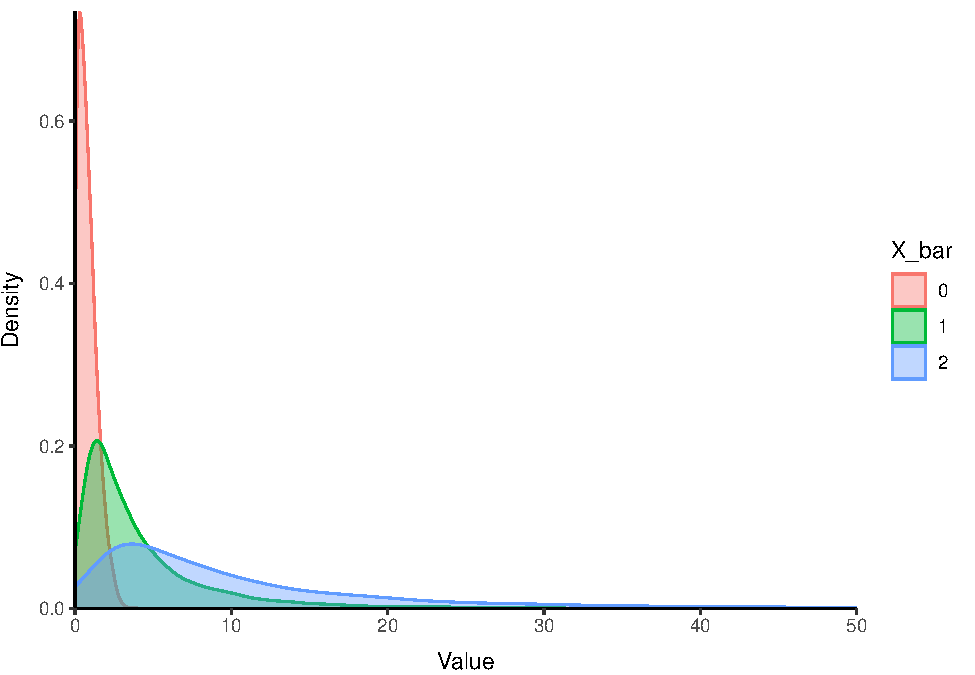
\includegraphics{worstr_files/figure-latex/unnamed-chunk-123-1.pdf}

You can see that the relative scale of these three distributions is similar, but the location shifts to the right on our x-axis as the value of \texttt{X\_bar} (the mean) increases. Note also how this affects \emph{kurtosis}.

\hypertarget{the-beta-distribution}{%
\subsection{The beta distribution}\label{the-beta-distribution}}

The \textbf{beta distribution} is a probability distribution that is constrained to the interval {[}0, 1{]}. But, it is incredibly flexible in its parameterization, and as a result is very useful for stochastic simulation of variables on the probability scale, such as survival.

The parameters of the beta distribution are \(\alpha\) and \(\beta\), or commonly \texttt{a} and \texttt{b} or \texttt{shape\ 1} and \texttt{shape\ 2} in R. Within this distribution, \(\alpha\) pushes the distribution to the right (toward 1), and \(\beta\) pushes the distribution back toward the left (toward 0). The relative magnitude of \(\alpha\) and \(\beta\) determine the location, shape, and scale of the probability distribution for our random variable. When \(\alpha\) and \(\beta\) are equal, and greater than 1, the beta distribution looks like a normal distribution within the interval {[}0, 1{]}.

Let's take a look:

\begin{Shaded}
\begin{Highlighting}[]
\CommentTok{# Simulate random values from 3 different beta distributions}
\CommentTok{# so we can compare them}
\NormalTok{samp1 <-}\StringTok{ }\KeywordTok{rbeta}\NormalTok{(}\DataTypeTok{n=}\FloatTok{1e4}\NormalTok{, }\DataTypeTok{shape1=}\DecValTok{50}\NormalTok{, }\DataTypeTok{shape2=}\DecValTok{50}\NormalTok{)}
\NormalTok{samp2 <-}\StringTok{ }\KeywordTok{rbeta}\NormalTok{(}\DataTypeTok{n=}\FloatTok{1e4}\NormalTok{, }\DataTypeTok{shape1=}\DecValTok{50}\NormalTok{, }\DataTypeTok{shape2=}\DecValTok{100}\NormalTok{)     }
\NormalTok{samp3 <-}\StringTok{ }\KeywordTok{rbeta}\NormalTok{(}\DataTypeTok{n=}\FloatTok{1e4}\NormalTok{, }\DataTypeTok{shape1=}\DecValTok{500}\NormalTok{, }\DataTypeTok{shape2=}\DecValTok{250}\NormalTok{) }

\CommentTok{# Put them in a data frame with the values}
\CommentTok{# of the means used to create them. I am }
\CommentTok{# using "theta" because often that is how we}
\CommentTok{# refer collectively to a group of parameters}
\NormalTok{betas <-}\StringTok{ }\KeywordTok{data.frame}\NormalTok{(}
  \DataTypeTok{Value =} \KeywordTok{c}\NormalTok{(samp, samp2, samp3),}
  \DataTypeTok{theta =} \KeywordTok{factor}\NormalTok{(}
    \KeywordTok{c}\NormalTok{(}
      \KeywordTok{rep}\NormalTok{(}\StringTok{'a = 50, b = 50'}\NormalTok{, }\KeywordTok{length}\NormalTok{(samp)), }
      \KeywordTok{rep}\NormalTok{(}\StringTok{'a = 50, b = 100'}\NormalTok{, }\KeywordTok{length}\NormalTok{(samp2)), }
      \KeywordTok{rep}\NormalTok{(}\StringTok{'a = 500, b = 250'}\NormalTok{, }\KeywordTok{length}\NormalTok{(samp3))}
\NormalTok{    )}
\NormalTok{  )}
\NormalTok{)}
\end{Highlighting}
\end{Shaded}

And then, we can plot them just like we did above. Copy and paste it - change what you need. Isn't code great?. Just don't forget to change the scale and the data in the plotting code!

\begin{Shaded}
\begin{Highlighting}[]
\NormalTok{p <-}\StringTok{ }\KeywordTok{ggplot}\NormalTok{(}\DataTypeTok{data =}\NormalTok{ betas,}
            \KeywordTok{aes}\NormalTok{(}\DataTypeTok{x =}\NormalTok{ Value, }\DataTypeTok{group =}\NormalTok{ theta, }\DataTypeTok{fill =}\NormalTok{ theta, }\DataTypeTok{color =}\NormalTok{ theta)) }\OperatorTok{+}
\StringTok{  }\KeywordTok{geom_density}\NormalTok{(}\DataTypeTok{adjust =} \FloatTok{1.5}\NormalTok{, }\DataTypeTok{alpha =} \FloatTok{.4}\NormalTok{) }\OperatorTok{+}
\StringTok{  }\KeywordTok{scale_x_continuous}\NormalTok{(}\DataTypeTok{limits =}\KeywordTok{c}\NormalTok{(}\DecValTok{0}\NormalTok{, }\DecValTok{1}\NormalTok{), }\DataTypeTok{expand =} \KeywordTok{c}\NormalTok{(}\DecValTok{0}\NormalTok{, }\DecValTok{0}\NormalTok{)) }\OperatorTok{+}\StringTok{ }
\StringTok{  }\KeywordTok{scale_y_continuous}\NormalTok{(}\DataTypeTok{expand =} \KeywordTok{c}\NormalTok{(}\DecValTok{0}\NormalTok{, }\DecValTok{0}\NormalTok{)) }\OperatorTok{+}\StringTok{ }
\StringTok{  }\KeywordTok{xlab}\NormalTok{(}\StringTok{"Value"}\NormalTok{) }\OperatorTok{+}
\StringTok{  }\KeywordTok{ylab}\NormalTok{(}\StringTok{"Density"}\NormalTok{) }\OperatorTok{+}
\StringTok{  }\KeywordTok{theme_classic}\NormalTok{() }\OperatorTok{+}
\StringTok{  }\KeywordTok{theme}\NormalTok{(}
    \DataTypeTok{axis.title.x =} \KeywordTok{element_text}\NormalTok{(}\DataTypeTok{vjust =} \DecValTok{-1}\NormalTok{),}
    \DataTypeTok{axis.title.y =} \KeywordTok{element_text}\NormalTok{(}\DataTypeTok{vjust =} \DecValTok{3}\NormalTok{),}
    \DataTypeTok{panel.grid =} \KeywordTok{element_blank}\NormalTok{()}
\NormalTok{  )}
\KeywordTok{print}\NormalTok{(p)}
\end{Highlighting}
\end{Shaded}

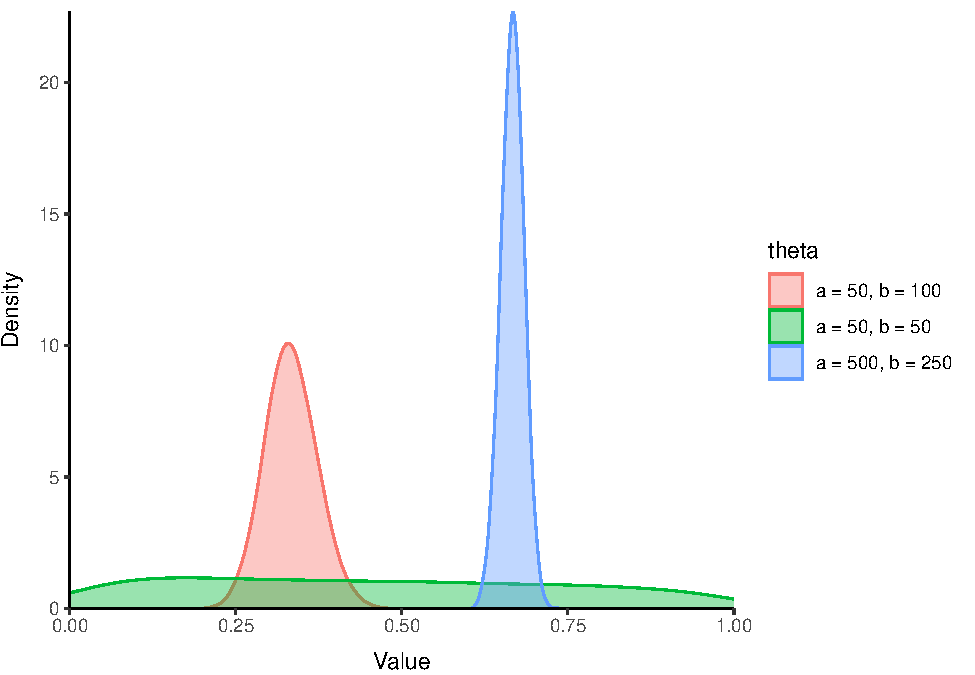
\includegraphics{worstr_files/figure-latex/unnamed-chunk-125-1.pdf}

Play around with these to see what kind of cool shapes you can make and where they are located within the range between zero and one.

\hypertarget{discrete-distributions}{%
\section{Discrete distributions}\label{discrete-distributions}}

\textbf{Discrete} probability distributions are useful for situations in which our random variable of interest can only take specific values within the interval of interest. For example, this might include age, counts, pass/fail, or any number of conceivable categories. As a result, these require a slightly different treatment of probability as a discrete, rather than continuous phenomenon. (Think back to our histogram that we started with in this chapter.)

\hypertarget{bernoulli}{%
\subsection{Bernoulli}\label{bernoulli}}

The \textbf{Bernoulli distribution} is a special case of the binomial distribution with a single trial (see below for clarification). Bernoulli outcomes are those for which the variable we are measuring can take on one of two values: a one or a zero. This distribution is useful for visualizing processes such as coin flips, yes/no responses, live/dead endpoints in lab studies, and a number of other very interesting phenomena. The Bernoulli distribution has a single parameter: the probability of success, but the number of successful outcomes is also governed by sample size: \emph{n}, which R calls \texttt{size} because \texttt{n} was already taken.

We can simulate data from a Bernoulli distribution in one of two ways in R.

The ``old-school'' way of doing this was to draw from a binomial with a single \textbf{trial}. Here we randomly draw a single sample from a binomial with a single trial, and a 50\% chance of success. We'll use the example of hatching chicken eggs with some probability of success. If you are boring, you can think about flipping coins, too!

We'll start with one chicken egg that has a 50\% chance of successfully hatching (probability of success = 0.50).

\begin{Shaded}
\begin{Highlighting}[]
\KeywordTok{rbinom}\NormalTok{(}\DataTypeTok{n=}\DecValTok{1}\NormalTok{, }\DataTypeTok{size=}\DecValTok{1}\NormalTok{, }\DataTypeTok{prob=}\NormalTok{.}\DecValTok{5}\NormalTok{)}
\end{Highlighting}
\end{Shaded}

\begin{verbatim}
## [1] 0
\end{verbatim}

There is also a function called \texttt{rbern} in the \texttt{Rlab} package that simplifies this for the specific case of a Bernoulli.

Let's do it again with that function:

\begin{Shaded}
\begin{Highlighting}[]
\CommentTok{# Hatch one egg with 50% success rate}
\KeywordTok{rbern}\NormalTok{(}\DataTypeTok{n =} \DecValTok{1}\NormalTok{, }\DataTypeTok{prob =} \FloatTok{.5}\NormalTok{)}
\end{Highlighting}
\end{Shaded}

\begin{verbatim}
## [1] 1
\end{verbatim}

Or we could hatch a whole bunch of eggs:

\begin{Shaded}
\begin{Highlighting}[]
\CommentTok{# Hatch ten eggs, each with p = 0.5}
\KeywordTok{rbern}\NormalTok{(}\DataTypeTok{n =} \DecValTok{10}\NormalTok{, }\DataTypeTok{prob =} \FloatTok{.5}\NormalTok{)}
\end{Highlighting}
\end{Shaded}

\begin{verbatim}
##  [1] 0 1 0 0 0 1 1 0 1 0
\end{verbatim}

Then, we could even count how many of those were successful. Do you remember how to do that? There are several different ways. You'll have to come up with one for the homework assignment (hint: see \protect\hyperlink{Chapter2}{Chapter 2}).

\hypertarget{binomial}{%
\subsection{Binomial}\label{binomial}}

The \textbf{binomial distribution} is pretty similar to the Bernoulli distribution. In fact, the Bernoulli is just a special kind of binomial. The binomial includes a parameter called \(N\) (\texttt{size} in R) which corresponds to a number of trials per sample. We assume that this is 1 in the case of Bernoulli. In most cases in biology, it will suffice to use the Bernoulli, but for modeling we will want to understand the binomial for things like random stratified designs and nested models that rely on the use of binomial distribution. Later in your career, you might even get into cool models that estimate \(N\) as a latent state to estimate population size (for example). Plus, using the binomial is way faster and can be more precise for certain regression applications {[}okay, that one should probably have a citation, but this is The Worst Stats Text eveR, so go Google it{]}.

To sample data from a binomial distribution, we can use \texttt{rbinom} from base R. In this example we tell R that we want 10 samples (\texttt{n}) from a binomial distribution that has 10 trials (\texttt{size}) and a probability of success (\texttt{prob}) of 0.5. This is like hatching ten eggs from each of ten chickens instead of just one chicken laying ten eggs.

\begin{Shaded}
\begin{Highlighting}[]
\CommentTok{# Take a random draw of 10 samples}
\CommentTok{# from a binomial distribution with 10 trials}
\CommentTok{# and probability of success equal to 0.50}
\KeywordTok{rbinom}\NormalTok{(}\DataTypeTok{n=}\DecValTok{10}\NormalTok{, }\DataTypeTok{size=}\DecValTok{10}\NormalTok{, }\DataTypeTok{prob=}\FloatTok{0.5}\NormalTok{)}
\end{Highlighting}
\end{Shaded}

\begin{verbatim}
##  [1] 4 5 5 7 6 3 5 5 5 3
\end{verbatim}

Remember as you look through these that your numbers should look different than mine (at least most of the time) because these are being generated randomly.

\hypertarget{multinomial}{%
\subsection{Multinomial}\label{multinomial}}

The \textbf{multinomial distribution} is a further generalization of the Binomial and Bernoulli distributions. Here, there are one or more possible categorical outcomes (states), and the probability of each one occurring is specified individually \textbf{but all of them must sum to one}. The categories are, in this case, assumed to be a \textbf{mutually exclusive} and \textbf{exhaustive} set of possible outcomes.

We can use the multinomial distribution to randomly sample from categories (imagine our response variable is a categorical variable, like the names of the students in this class).

To do this, we need to read in the \texttt{s\_names.csv} file from our \texttt{data} folder that is definitely in your working directory (\textbf{remember to set your working directory first}).

Read in the data file with \texttt{stringsAsFactors\ =\ FALSE} for purposes of demonstrating with categorical variables (not factors).

\begin{Shaded}
\begin{Highlighting}[]
\NormalTok{s_names <-}\StringTok{ }\KeywordTok{read.csv}\NormalTok{(}\StringTok{'data/s_names.csv'}\NormalTok{, }\DataTypeTok{stringsAsFactors =} \OtherTok{FALSE}\NormalTok{)}
\end{Highlighting}
\end{Shaded}

Next, let's assign the variable \texttt{name} in \texttt{s\_names} to a vector for simplicity.

\begin{Shaded}
\begin{Highlighting}[]
\NormalTok{name <-}\StringTok{ }\NormalTok{s_names}\OperatorTok{$}\NormalTok{name}
\end{Highlighting}
\end{Shaded}

Then, we can assign a uniform probability of drawing any given name if we divide one by the number of names.

\begin{Shaded}
\begin{Highlighting}[]
\CommentTok{# Calculate probability of getting a given }
\CommentTok{# name based on the length of the vector}
\NormalTok{prob_each <-}\StringTok{ }\DecValTok{1} \OperatorTok{/}\StringTok{ }\KeywordTok{length}\NormalTok{(name)}

\CommentTok{# Repeat this probability for each }
\CommentTok{# name in our vector of names}
\NormalTok{probs <-}\StringTok{ }\KeywordTok{rep}\NormalTok{(prob_each, }\DataTypeTok{times =} \KeywordTok{length}\NormalTok{(name))      }
\NormalTok{probs      }
\end{Highlighting}
\end{Shaded}

\begin{verbatim}
##  [1] 0.03846154 0.03846154 0.03846154 0.03846154 0.03846154 0.03846154
##  [7] 0.03846154 0.03846154 0.03846154 0.03846154 0.03846154 0.03846154
## [13] 0.03846154 0.03846154 0.03846154 0.03846154 0.03846154 0.03846154
## [19] 0.03846154 0.03846154 0.03846154 0.03846154 0.03846154 0.03846154
## [25] 0.03846154 0.03846154
\end{verbatim}

This shows us that the probability of drawing any of the individual names is \texttt{\{r\ prob\_each\}}.

Now, we can sample from a multinomial distribution using our objects. Here we are taking 5 samples from the distribution, each time we sample there is only one trial, and we are sampling with the 26 probabilities above.

Have a look:

\begin{Shaded}
\begin{Highlighting}[]
\KeywordTok{rmultinom}\NormalTok{(}\DataTypeTok{n=}\DecValTok{5}\NormalTok{, }\DataTypeTok{size=}\DecValTok{1}\NormalTok{, }\DataTypeTok{prob=}\NormalTok{probs)}
\end{Highlighting}
\end{Shaded}

\begin{verbatim}
##       [,1] [,2] [,3] [,4] [,5]
##  [1,]    0    0    1    0    0
##  [2,]    0    0    0    0    0
##  [3,]    0    0    0    0    0
##  [4,]    0    0    0    0    0
##  [5,]    0    0    0    0    1
##  [6,]    0    0    0    0    0
##  [7,]    0    0    0    1    0
##  [8,]    0    0    0    0    0
##  [9,]    0    0    0    0    0
## [10,]    0    0    0    0    0
## [11,]    0    0    0    0    0
## [12,]    0    0    0    0    0
## [13,]    1    0    0    0    0
## [14,]    0    0    0    0    0
## [15,]    0    0    0    0    0
## [16,]    0    0    0    0    0
## [17,]    0    0    0    0    0
## [18,]    0    0    0    0    0
## [19,]    0    0    0    0    0
## [20,]    0    0    0    0    0
## [21,]    0    0    0    0    0
## [22,]    0    1    0    0    0
## [23,]    0    0    0    0    0
## [24,]    0    0    0    0    0
## [25,]    0    0    0    0    0
## [26,]    0    0    0    0    0
\end{verbatim}

\textbf{WHOA} a matrix??!!! \textbf{What does it all mean}?

Take a step back, breathe, and think about this. The rows in this matrix are you and your classmates. If we took one random sample from the multinomial distribution, it would look like this:

\begin{Shaded}
\begin{Highlighting}[]
\CommentTok{# Take a single sample from}
\CommentTok{# the list of student names    }
\KeywordTok{rmultinom}\NormalTok{(}\DataTypeTok{n=}\DecValTok{1}\NormalTok{, }\DataTypeTok{size=}\DecValTok{1}\NormalTok{, }\DataTypeTok{prob=}\NormalTok{probs)}
\end{Highlighting}
\end{Shaded}

\begin{verbatim}
##       [,1]
##  [1,]    0
##  [2,]    0
##  [3,]    0
##  [4,]    0
##  [5,]    0
##  [6,]    0
##  [7,]    0
##  [8,]    0
##  [9,]    0
## [10,]    0
## [11,]    0
## [12,]    0
## [13,]    0
## [14,]    0
## [15,]    0
## [16,]    0
## [17,]    0
## [18,]    0
## [19,]    0
## [20,]    0
## [21,]    0
## [22,]    0
## [23,]    1
## [24,]    0
## [25,]    0
## [26,]    0
\end{verbatim}

Here, we pulled a single sample from the distribution, and probability of sampling a given individual was 0.04 (1/26). If it makes it easier, we can put your names next to it:

\begin{Shaded}
\begin{Highlighting}[]
\KeywordTok{cbind}\NormalTok{(name, }\KeywordTok{rmultinom}\NormalTok{(}\DataTypeTok{n=}\DecValTok{1}\NormalTok{, }\DataTypeTok{size=}\DecValTok{1}\NormalTok{, }\DataTypeTok{prob=}\NormalTok{probs))}
\end{Highlighting}
\end{Shaded}

\begin{verbatim}
##       name             
##  [1,] "Ava"         "0"
##  [2,] "Dillon"      "0"
##  [3,] "Delaney"     "0"
##  [4,] "Manolo"      "0"
##  [5,] "Sarah"       "0"
##  [6,] "Shannon"     "0"
##  [7,] "Olivia"      "0"
##  [8,] "Ebony"       "0"
##  [9,] "Julia"       "0"
## [10,] "Davi"        "0"
## [11,] "Gabrielle"   "0"
## [12,] "Jordan"      "0"
## [13,] "Tayler"      "0"
## [14,] "Summer"      "0"
## [15,] "Leah"        "0"
## [16,] "Christine"   "0"
## [17,] "Ashley"      "0"
## [18,] "Katherine"   "0"
## [19,] "James"       "0"
## [20,] "Emily"       "0"
## [21,] "Cassidy"     "0"
## [22,] "Maximillion" "0"
## [23,] "Sierra"      "1"
## [24,] "Kyle"        "0"
## [25,] "Diana"       "0"
## [26,] "Amanda"      "0"
\end{verbatim}

Now, if I was calling on you randomly in class, after 10 questions, the spread of people who would have participated in class might look like this (or whatever you got - remember, it is random):

\begin{Shaded}
\begin{Highlighting}[]
\KeywordTok{cbind}\NormalTok{(name, }\KeywordTok{rmultinom}\NormalTok{(}\DataTypeTok{n=}\DecValTok{10}\NormalTok{, }\DataTypeTok{size=}\DecValTok{1}\NormalTok{, }\DataTypeTok{prob=}\NormalTok{probs))}
\end{Highlighting}
\end{Shaded}

\begin{verbatim}
##       name                                                 
##  [1,] "Ava"         "0" "0" "0" "0" "1" "0" "0" "0" "0" "0"
##  [2,] "Dillon"      "0" "1" "0" "0" "0" "0" "0" "0" "0" "0"
##  [3,] "Delaney"     "1" "0" "0" "0" "0" "0" "0" "0" "0" "0"
##  [4,] "Manolo"      "0" "0" "0" "0" "0" "0" "0" "0" "0" "1"
##  [5,] "Sarah"       "0" "0" "0" "0" "0" "0" "0" "0" "0" "0"
##  [6,] "Shannon"     "0" "0" "0" "0" "0" "0" "0" "0" "0" "0"
##  [7,] "Olivia"      "0" "0" "0" "0" "0" "0" "0" "0" "0" "0"
##  [8,] "Ebony"       "0" "0" "0" "0" "0" "0" "0" "0" "0" "0"
##  [9,] "Julia"       "0" "0" "0" "0" "0" "0" "0" "0" "0" "0"
## [10,] "Davi"        "0" "0" "1" "0" "0" "0" "0" "0" "0" "0"
## [11,] "Gabrielle"   "0" "0" "0" "0" "0" "1" "0" "0" "0" "0"
## [12,] "Jordan"      "0" "0" "0" "0" "0" "0" "0" "0" "0" "0"
## [13,] "Tayler"      "0" "0" "0" "0" "0" "0" "0" "0" "0" "0"
## [14,] "Summer"      "0" "0" "0" "0" "0" "0" "0" "0" "0" "0"
## [15,] "Leah"        "0" "0" "0" "0" "0" "0" "0" "0" "0" "0"
## [16,] "Christine"   "0" "0" "0" "0" "0" "0" "0" "0" "0" "0"
## [17,] "Ashley"      "0" "0" "0" "0" "0" "0" "0" "0" "0" "0"
## [18,] "Katherine"   "0" "0" "0" "0" "0" "0" "0" "0" "0" "0"
## [19,] "James"       "0" "0" "0" "0" "0" "0" "0" "0" "0" "0"
## [20,] "Emily"       "0" "0" "0" "0" "0" "0" "0" "0" "0" "0"
## [21,] "Cassidy"     "0" "0" "0" "0" "0" "0" "0" "0" "1" "0"
## [22,] "Maximillion" "0" "0" "0" "1" "0" "0" "0" "0" "0" "0"
## [23,] "Sierra"      "0" "0" "0" "0" "0" "0" "1" "1" "0" "0"
## [24,] "Kyle"        "0" "0" "0" "0" "0" "0" "0" "0" "0" "0"
## [25,] "Diana"       "0" "0" "0" "0" "0" "0" "0" "0" "0" "0"
## [26,] "Amanda"      "0" "0" "0" "0" "0" "0" "0" "0" "0" "0"
\end{verbatim}

Taking this one step further, we could just draw a name and stop looking at these ugly (no but really they are \textbf{awesome}!) matrices:

\begin{Shaded}
\begin{Highlighting}[]
\NormalTok{name[}\KeywordTok{which}\NormalTok{(}\KeywordTok{rmultinom}\NormalTok{(}\DataTypeTok{n=}\DecValTok{1}\NormalTok{, }\DataTypeTok{size=}\DecValTok{1}\NormalTok{, }\DataTypeTok{prob=}\NormalTok{probs)}\OperatorTok{>}\DecValTok{0}\NormalTok{)]}
\end{Highlighting}
\end{Shaded}

\begin{verbatim}
## [1] "Amanda"
\end{verbatim}

And now we have a way to randomly select an individual based on a multinomial distribution. What fun!

\hypertarget{poisson}{%
\subsection{Poisson}\label{poisson}}

The \textbf{Poisson distribution} is used for counts or other integer data. This distribution is widely used (and just as widely misused!) for its ability to account for a large number of biological and ecological processes in the models that we will discuss this semester. The Poisson distribution has a single parameter, \(\lambda\), which is both the mean and the variance of the distribution. So, despite its utility, the distribution is relatively inflexible with respect to shape and spread. \textbf{Fun fact}: this distribution was made widely known by a Russian economist to predict the number of soldiers who were accidentally killed from being kicked by horses in the Prussian army each year. It is named, however, after French mathematician Siméon Denis Poisson. {[}fails to provide citations for any of this{]}

Take a look at how the distribution changes when you change \(\lambda\), and you will get an idea of how this one works. It is probably the most straightforward of any we've considered.

\begin{Shaded}
\begin{Highlighting}[]
\KeywordTok{hist}\NormalTok{(}\KeywordTok{rpois}\NormalTok{(}\DataTypeTok{n=}\FloatTok{1e4}\NormalTok{, }\DataTypeTok{lambda=}\DecValTok{100}\NormalTok{), }\DataTypeTok{main=}\StringTok{''}\NormalTok{)}
\end{Highlighting}
\end{Shaded}

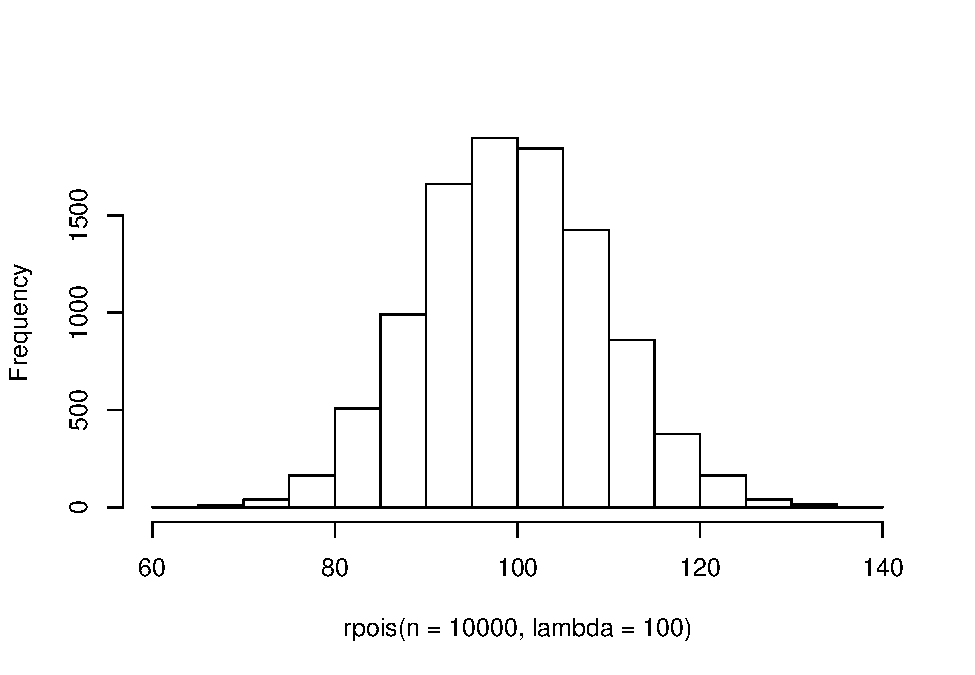
\includegraphics{worstr_files/figure-latex/unnamed-chunk-138-1.pdf}

We'll set it aside for now because it often fails us (or our data fail it, I suppose).

\hypertarget{the-negative-binomial-distribution}{%
\subsection{The negative binomial distribution}\label{the-negative-binomial-distribution}}

Okay, this one can be a little difficult to wrap your head around but it's an important one for us to know about. So, we will spend a little extra time setting this one up to try and be clear. Often, folks start out thinking that they're going to use a Poisson distribution and they end up collecting with data that do not conform to the relative inflexibility of that single-parameter distribution. Where they end up usually tends to be a negative binomial in a best case (we'll talk about challenges associated with lots of zeros later in the book).

For the purpose of this class, we are not going to dive into the mechanics of the \textbf{negative binomial distribution}, but we do need to know what it looks like and why we might need it.

One useful way to conceptualize the negative binomial is ``how long does it take for some event to occur?'' For example, we might ask how long it takes a fish to start migrating, how long it takes a sea turtle to recover in a rehabilitation center, how long it will take for a terminal patient to expire (ooh, that's dark), or how frequently we see the expression of a gene of interest. These kinds of questions are asked in aptly named ``time-to-event'' models that rely on the variance structure of the negative binomial. In the context of these kinds of questions, the negative binomial is a discrete probability distribution (and not a continuous distribution) because the ``time'' component of the distribution is actually a series of independent Bernoulli trials (holy crap!). For example: if we want to know how many days it will take for a turtle to recover from an injury, what we are really doing is asking on each day until recovery, ``Is today the day?''. Then, we flip a coin and find out. So, each day in this example is a Bernoulli trial. Another way to think about this is the number of failures occurring in a sequence before a target number of sucesses is achieved.

For the classical parameterization:

We will start by looking at how many failures are observed before one success in a sequence of Bernoulli trials.

With probability of succes equal to 0.95, it doesn't take long and most of the probability mass is near zero, with a couple of stragglers further out.

\begin{Shaded}
\begin{Highlighting}[]
\CommentTok{# Take a random sample from the negative binomial}
\NormalTok{Value <-}\StringTok{ }\KeywordTok{rnbinom}\NormalTok{(}\FloatTok{1e4}\NormalTok{, }\DataTypeTok{size=}\DecValTok{1}\NormalTok{, }\DataTypeTok{prob=}\NormalTok{.}\DecValTok{95}\NormalTok{)}

\CommentTok{# Make a histogram of it with ggplot}
\KeywordTok{ggplot}\NormalTok{() }\OperatorTok{+}\StringTok{ }\KeywordTok{geom_histogram}\NormalTok{( }\KeywordTok{aes}\NormalTok{(}\DataTypeTok{x =}\NormalTok{ Value) )}
\end{Highlighting}
\end{Shaded}

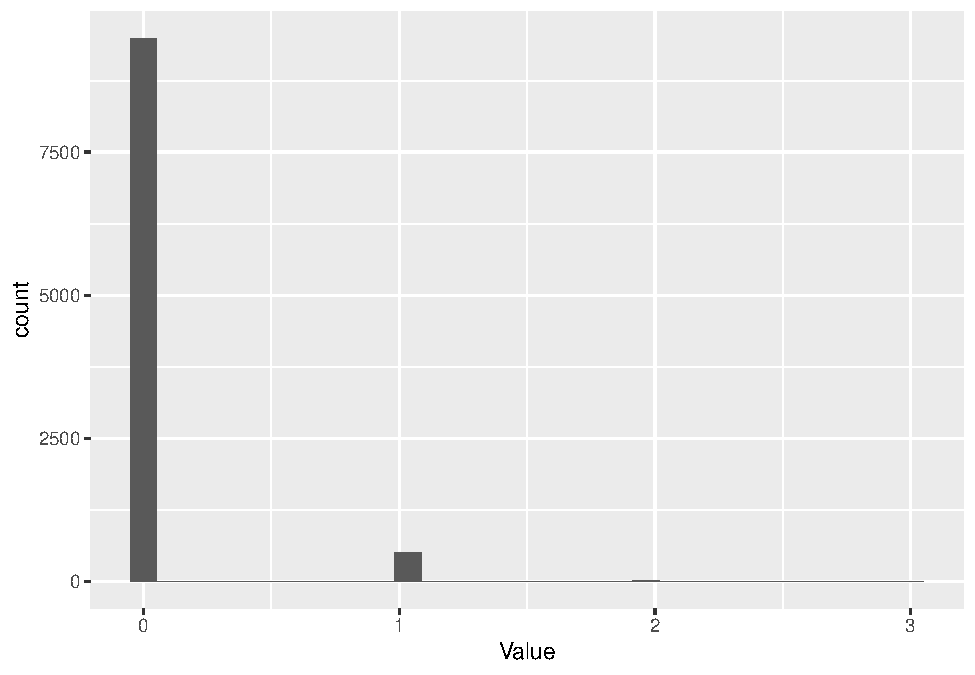
\includegraphics{worstr_files/figure-latex/unnamed-chunk-139-1.pdf}

If we decrease probability of success in each trial to 0.25, we see more failures on average before we reach success. Most of the time, it still takes less than 5 trials to reach a success, but some times it takes much longer.

\begin{Shaded}
\begin{Highlighting}[]
\CommentTok{# Take a random sample from the negative binomial}
\NormalTok{Value <-}\StringTok{ }\KeywordTok{rnbinom}\NormalTok{(}\FloatTok{1e4}\NormalTok{, }\DataTypeTok{size=}\DecValTok{1}\NormalTok{, }\DataTypeTok{prob=}\NormalTok{.}\DecValTok{25}\NormalTok{)}

\CommentTok{# Make a histogram of it with ggplot}
\KeywordTok{ggplot}\NormalTok{() }\OperatorTok{+}\StringTok{ }\KeywordTok{geom_histogram}\NormalTok{( }\KeywordTok{aes}\NormalTok{(}\DataTypeTok{x =}\NormalTok{ Value) )}
\end{Highlighting}
\end{Shaded}

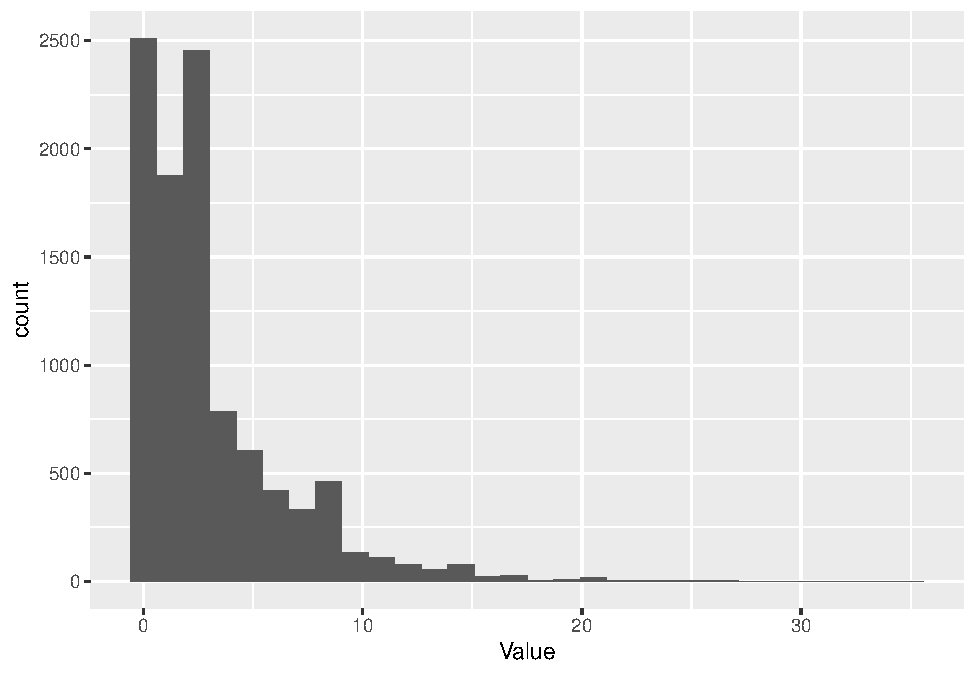
\includegraphics{worstr_files/figure-latex/unnamed-chunk-140-1.pdf}

And, if we increase the number of successes that we use for our criterion, or target, then it spreads the distribution out even further.

\begin{Shaded}
\begin{Highlighting}[]
\CommentTok{# Take a random sample from the negative binomial}
\NormalTok{Value <-}\StringTok{ }\KeywordTok{rnbinom}\NormalTok{(}\FloatTok{1e4}\NormalTok{, }\DataTypeTok{size=}\DecValTok{10}\NormalTok{, }\DataTypeTok{prob=}\NormalTok{.}\DecValTok{25}\NormalTok{)}

\CommentTok{# Make a histogram of it with ggplot}
\KeywordTok{ggplot}\NormalTok{() }\OperatorTok{+}\StringTok{ }\KeywordTok{geom_histogram}\NormalTok{( }\KeywordTok{aes}\NormalTok{(}\DataTypeTok{x =}\NormalTok{ Value) )}
\end{Highlighting}
\end{Shaded}

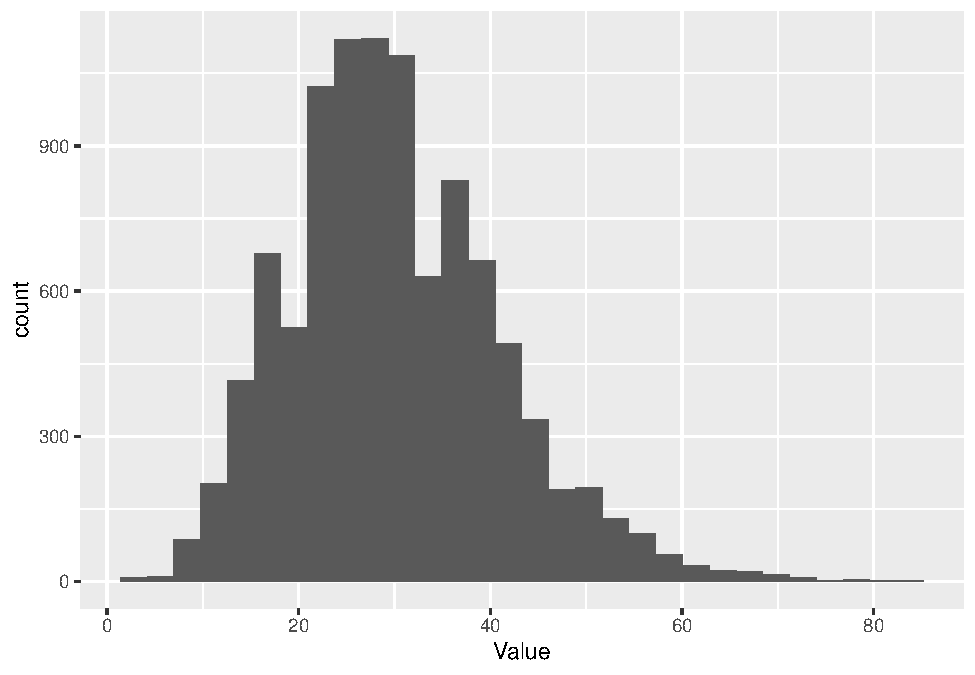
\includegraphics{worstr_files/figure-latex/unnamed-chunk-141-1.pdf}

Now, because of it's properties, the negative binomial is also useful for number of other applications that have nothing to do with interpretting the results of repeated binomial trials. Specifically, it has been widely used to represent Poisson-like processes in which the mean and variance are not equal (e.g., \textbf{overdispersion}). This has seen a lot of application in the field of ecology, especially for overdispersed count data.

Here, we draw 10,000 random samples from a negative binomial distribution with a mean of 10 and an overdispersion parameter of 1. The overdispersion parameter is called `size' because this is an alternative parameterization that is just making use of the relationships between existing parameters of the negative binomial. It's easy to grasp how the mean changes the location of the distribution.

\begin{Shaded}
\begin{Highlighting}[]
\CommentTok{# Take a random sample from the negative binomial}
\NormalTok{Value <-}\StringTok{ }\KeywordTok{rnbinom}\NormalTok{(}\FloatTok{1e4}\NormalTok{, }\DataTypeTok{mu =} \DecValTok{10}\NormalTok{, }\DataTypeTok{size =} \DecValTok{1}\NormalTok{)}

\CommentTok{# Make a histogram of it with ggplot}
\KeywordTok{ggplot}\NormalTok{() }\OperatorTok{+}\StringTok{ }\KeywordTok{geom_histogram}\NormalTok{( }\KeywordTok{aes}\NormalTok{(}\DataTypeTok{x =}\NormalTok{ Value), }\DataTypeTok{bins =} \DecValTok{20}\NormalTok{ )}
\end{Highlighting}
\end{Shaded}

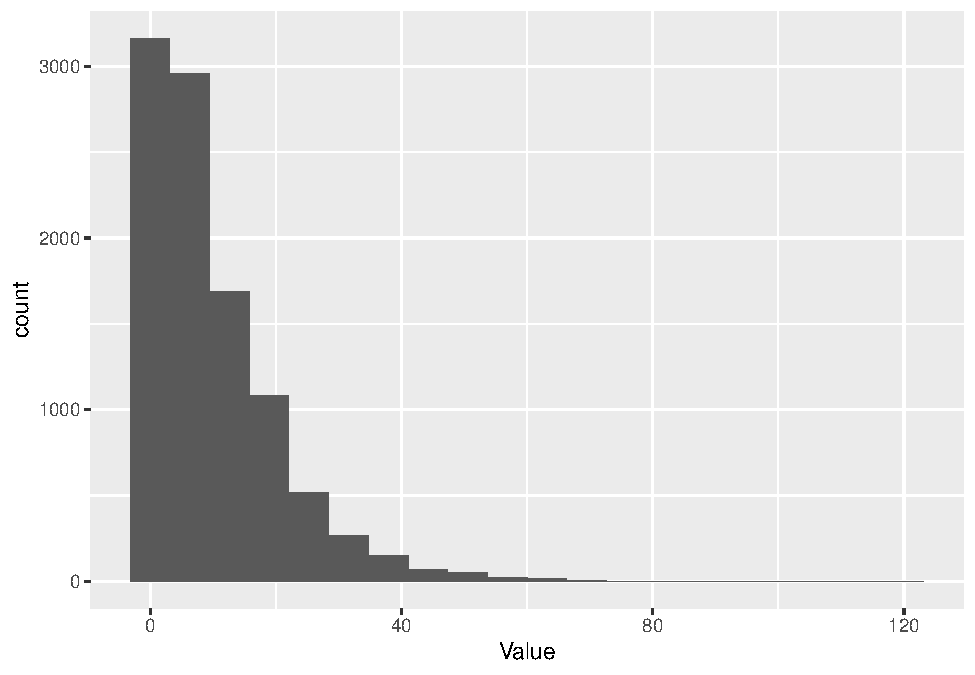
\includegraphics{worstr_files/figure-latex/unnamed-chunk-142-1.pdf}

But, note how the overdispersion parameter changes things if you run the following code:

\begin{Shaded}
\begin{Highlighting}[]
\CommentTok{# Take a random sample from the negative binomial}
\NormalTok{Value <-}\StringTok{ }\KeywordTok{rnbinom}\NormalTok{(}\FloatTok{1e4}\NormalTok{, }\DataTypeTok{mu =} \DecValTok{10}\NormalTok{, }\DataTypeTok{size =} \DecValTok{1000}\NormalTok{)}

\CommentTok{# Make a histogram of it with ggplot}
\KeywordTok{ggplot}\NormalTok{() }\OperatorTok{+}\StringTok{ }\KeywordTok{geom_histogram}\NormalTok{( }\KeywordTok{aes}\NormalTok{(}\DataTypeTok{x =}\NormalTok{ Value), }\DataTypeTok{bins =} \DecValTok{20}\NormalTok{ )}
\end{Highlighting}
\end{Shaded}

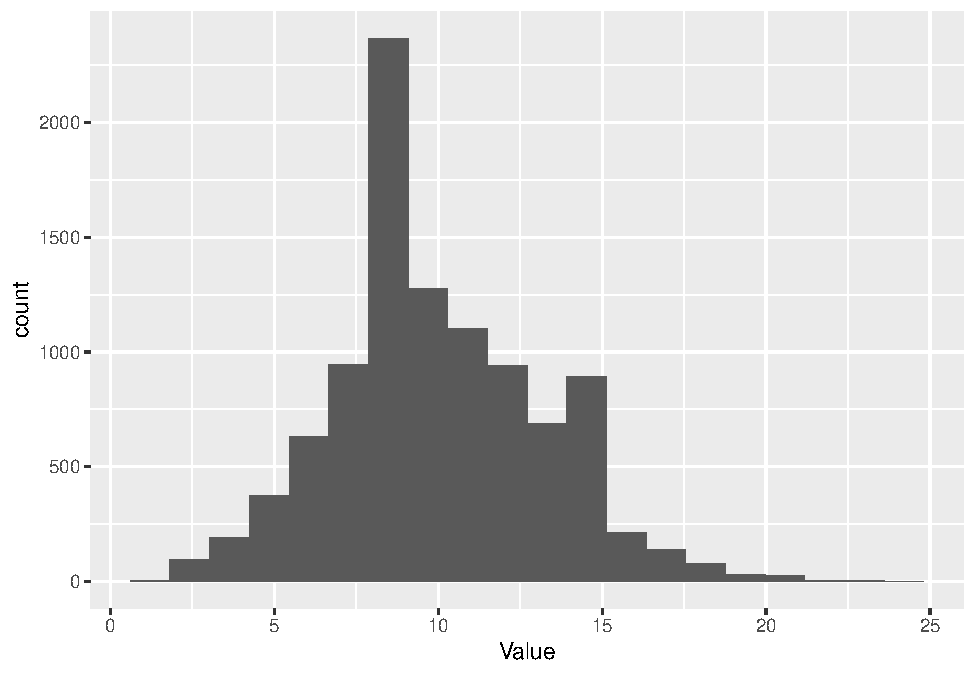
\includegraphics{worstr_files/figure-latex/unnamed-chunk-143-1.pdf}

A more intuitive way (I think) to work with the negative binomial in R is by using the \texttt{MASS} package. In this parameterization, we use the mean and the
dispersion parameter explicitly so it makes more sense:

\begin{Shaded}
\begin{Highlighting}[]
\CommentTok{# Take a random sample from the negative binomial}
\NormalTok{Value <-}\StringTok{ }\KeywordTok{rnegbin}\NormalTok{(}\FloatTok{1e4}\NormalTok{, }\DataTypeTok{mu =} \DecValTok{10}\NormalTok{, }\DataTypeTok{theta =} \DecValTok{1000}\NormalTok{)}

\CommentTok{# Make a histogram of it with ggplot}
\KeywordTok{ggplot}\NormalTok{() }\OperatorTok{+}\StringTok{ }\KeywordTok{geom_histogram}\NormalTok{( }\KeywordTok{aes}\NormalTok{(}\DataTypeTok{x =}\NormalTok{ Value), }\DataTypeTok{bins =} \DecValTok{20}\NormalTok{ )}
\end{Highlighting}
\end{Shaded}

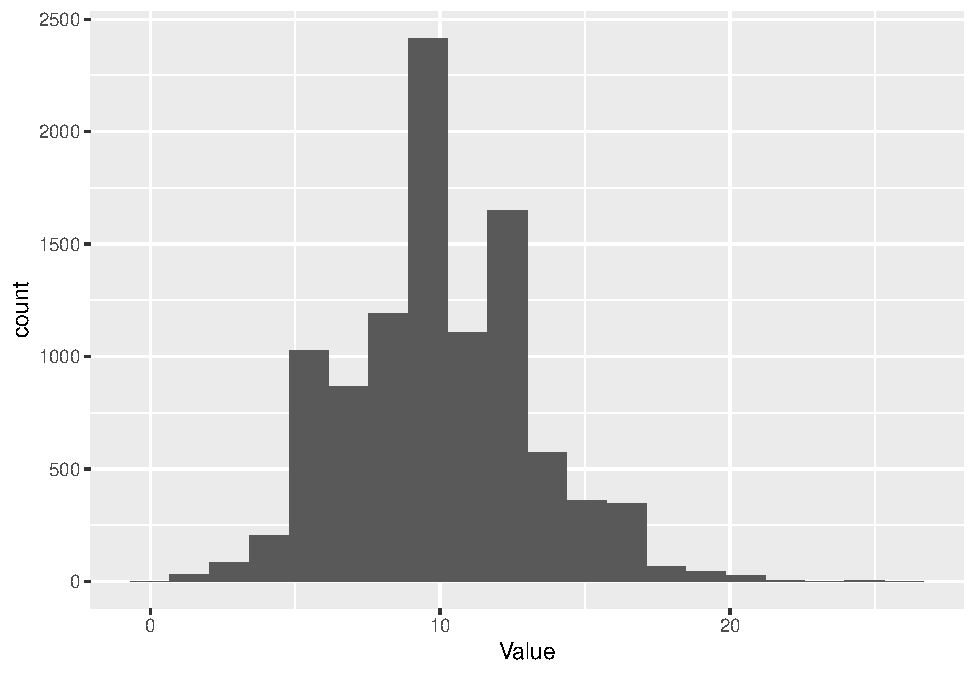
\includegraphics{worstr_files/figure-latex/unnamed-chunk-144-1.pdf}

The results are pretty much identical. Just two different naming systems for the parameters.

\hypertarget{sample-statistics}{%
\section{Sample statistics}\label{sample-statistics}}

In this section, we will learn how to derive the parameters of the \textbf{normal distribution} using a few different methods in R. We will use this opportunity to re-introduce the parameters as \textbf{moments} of the distribution so we can talk about what we mean by \textbf{confidence intervals}. We also will introduce a couple of different methods for calculating moments of a distribution. Specifically, we will look at how to derive\ldots{}

\hypertarget{moments-about-the-mean}{%
\subsection{Moments about the mean}\label{moments-about-the-mean}}

Sounds fancy, huh? Here they are, like a bandaid:

\begin{enumerate}
\def\labelenumi{\arabic{enumi}.}
\tightlist
\item
  Zeroth moment

  \begin{itemize}
  \tightlist
  \item
    This is the sum of the total probability of the distribution 1.00, always
  \end{itemize}
\item
  First moment

  \begin{itemize}
  \tightlist
  \item
    The mean
  \item
    We will look at a few ways to calculate this
  \end{itemize}
\item
  Second moment

  \begin{itemize}
  \tightlist
  \item
    The variance
  \item
    As with the mean, we will examine a couple of options for calculating
  \end{itemize}
\item
  Third moment

  \begin{itemize}
  \tightlist
  \item
    Skew
  \item
    We won't calculate for this class, but we have discussed, and this
    parameter contributes to the location/spread of the distribution (how
    far left or right the peak is)
  \end{itemize}
\item
  Fourth moment

  \begin{itemize}
  \tightlist
  \item
    Kurtosis
  \item
    Similarly, we won't cover the calculation, but this is another moment
    that we may have discussed with respect to departure from a z\\
    distribution in the normal
  \end{itemize}
\end{enumerate}

\hypertarget{estimating-parameters-of-the-normal-distribution-from-a-sample}{%
\subsection{Estimating parameters of the normal distribution from a sample}\label{estimating-parameters-of-the-normal-distribution-from-a-sample}}

The tools demonstrated below can be used for most of the probability distributions that have been implemented in R, and we could go on and on forever about them. But, for the sake of our collective sanity we will walk through the tools available using the normal distribution alone. Most of the time this will suffice because our objective in understanding other distributions is really just so that we can use them to assume asymptotic normality in response variables (with transformations) or parameter distributions (with link functions) later on anyway.

\hypertarget{method-of-moments-estimator}{%
\subsubsection{Method of moments estimator}\label{method-of-moments-estimator}}

The moments of the normal distribution are well defined, and you are probably familiar with how to calculate a mean (average) already. See if you can rearrange this in a way that makes sense with how you know to calculate a \textbf{mean} and a \textbf{variance}!

Start by simulating a variable with a known mean and standard deviation. We'll pretend that we are simulating cold temperatures here:

\begin{Shaded}
\begin{Highlighting}[]
\CommentTok{# Take a random sample from a normal}
\CommentTok{# with a mean of 20 and a standard}
\CommentTok{# deviation of 2}
\NormalTok{test_norm <-}\StringTok{ }\KeywordTok{rnorm}\NormalTok{(}\FloatTok{1e4}\NormalTok{, }\DecValTok{20}\NormalTok{, }\DecValTok{2}\NormalTok{)}
\end{Highlighting}
\end{Shaded}

First, we'll estimate it by making our own function:

\begin{Shaded}
\begin{Highlighting}[]
\CommentTok{# Write the function}
\CommentTok{# First, define a function by name}
\NormalTok{norm.mom =}\StringTok{ }\ControlFlowTok{function}\NormalTok{(x)\{      }
  
  \CommentTok{# Calculate mean}
\NormalTok{  x_bar =}\StringTok{ }\NormalTok{(}\DecValTok{1}\OperatorTok{/}\KeywordTok{length}\NormalTok{(x)) }\OperatorTok{*}\StringTok{ }\KeywordTok{sum}\NormalTok{(x) }
  
  \CommentTok{# Calculate variance}
\NormalTok{  sigma2 =}\StringTok{ }\NormalTok{(}\DecValTok{1}\OperatorTok{/}\KeywordTok{length}\NormalTok{(x)) }\OperatorTok{*}\StringTok{ }\KeywordTok{sum}\NormalTok{((x}\OperatorTok{-}\NormalTok{x_bar)}\OperatorTok{^}\DecValTok{2}\NormalTok{)}
  
  \CommentTok{# Return the calculations}
  \KeywordTok{return}\NormalTok{(}\KeywordTok{c}\NormalTok{(x_bar, sigma2))      }
  
\NormalTok{\}}
\CommentTok{# Test the function}
\KeywordTok{norm.mom}\NormalTok{(test_norm)}
\end{Highlighting}
\end{Shaded}

\begin{verbatim}
## [1] 19.970094  3.990084
\end{verbatim}

Because this one is so common, R has built-in estimators that rely on
the exact solution provided by the formulas for the first two moments
of the normal distribution:

\begin{Shaded}
\begin{Highlighting}[]
\KeywordTok{mean}\NormalTok{(test_norm)}
\end{Highlighting}
\end{Shaded}

\begin{verbatim}
## [1] 19.97009
\end{verbatim}

\begin{Shaded}
\begin{Highlighting}[]
\KeywordTok{var}\NormalTok{(test_norm)}
\end{Highlighting}
\end{Shaded}

\begin{verbatim}
## [1] 3.990483
\end{verbatim}

Wow, that was a lot less code. That is the beauty of having these functions available. How do these compare to the answers returned by our function if you scroll back up?

\hypertarget{maximum-likelihood-estimator}{%
\subsubsection{Maximum likelihood estimator}\label{maximum-likelihood-estimator}}

R also has built-in \textbf{maximum likelihood} estimators that provide an exact solution to the first two moments of the normal distribution. These are available through the \texttt{MASS} package.

\begin{Shaded}
\begin{Highlighting}[]
\KeywordTok{fitdistr}\NormalTok{(test_norm, }\StringTok{'normal'}\NormalTok{)}
\end{Highlighting}
\end{Shaded}

\begin{verbatim}
##       mean           sd     
##   19.97009390    1.99751941 
##  ( 0.01997519) ( 0.01412460)
\end{verbatim}

Only one problem here: R doesn't report the second moment! It reports
the square root of the second moment: the \textbf{standard deviation}!

Finally, let's write our own function and maximize the likelihood with the \texttt{optim()} function in R.

\begin{Shaded}
\begin{Highlighting}[]
\CommentTok{# Define the function}
\NormalTok{normal.lik =}\StringTok{ }\ControlFlowTok{function}\NormalTok{(theta, y)\{}
  
  \CommentTok{# The starting value for}
  \CommentTok{# mu that we provide}
\NormalTok{  mu =}\StringTok{ }\NormalTok{theta[}\DecValTok{1}\NormalTok{]}
  
  \CommentTok{# The starting value for}
  \CommentTok{# sigma2 that we provide}
\NormalTok{  sigma2 =}\StringTok{ }\NormalTok{theta[}\DecValTok{2}\NormalTok{]}
  
  \CommentTok{# Number of observations in the data}
\NormalTok{  n =}\StringTok{ }\KeywordTok{nrow}\NormalTok{(y)}
  
  \CommentTok{# Compute the log likelihood of the}
  \CommentTok{# data (y) using the likelihood}
  \CommentTok{# function for the normal distribution}
  \CommentTok{# given the starting values for our}
  \CommentTok{# parameters (contained in the vector 'theta')}
\NormalTok{  logl =}\StringTok{ }\FloatTok{-.5}\OperatorTok{*}\NormalTok{n}\OperatorTok{*}\KeywordTok{log}\NormalTok{(}\DecValTok{2}\OperatorTok{*}\NormalTok{pi) }\FloatTok{-.5}\OperatorTok{*}\NormalTok{n}\OperatorTok{*}\KeywordTok{log}\NormalTok{(sigma2)}\OperatorTok{-}\NormalTok{(}\DecValTok{1}\OperatorTok{/}\NormalTok{(}\DecValTok{2}\OperatorTok{*}\NormalTok{sigma2))}\OperatorTok{*}\KeywordTok{sum}\NormalTok{((y}\OperatorTok{-}\NormalTok{mu)}\OperatorTok{**}\DecValTok{2}\NormalTok{)}
  \KeywordTok{return}\NormalTok{(}\OperatorTok{-}\NormalTok{logl)}
\NormalTok{\}}
\end{Highlighting}
\end{Shaded}

Now, we use the \texttt{optim} function to maximize the likelihood of the data
(technically by minimizing the -2*log{[}likehood{]}) given different values of
our parameters (\texttt{mu} and \texttt{sigma2}).

To get started, we need to take a guess at what those parameters could be. (Yes, we know they are mu = 20 and sd = 2)

\begin{Shaded}
\begin{Highlighting}[]
\KeywordTok{optim}\NormalTok{(}\KeywordTok{c}\NormalTok{(}\DecValTok{20}\NormalTok{, }\DecValTok{4}\NormalTok{), normal.lik, }\DataTypeTok{y=}\KeywordTok{data.frame}\NormalTok{(test_norm))}
\end{Highlighting}
\end{Shaded}

\begin{verbatim}
## $par
## [1] 19.969855  3.991037
## 
## $value
## [1] 21108.45
## 
## $counts
## function gradient 
##       47       NA 
## 
## $convergence
## [1] 0
## 
## $message
## NULL
\end{verbatim}

The pieces are in \texttt{pars} here (right where we told R to put them!). We can also make the output into an object and call the parts by name:

\begin{Shaded}
\begin{Highlighting}[]
\CommentTok{# Make it into an object}
\NormalTok{est =}\StringTok{ }\KeywordTok{optim}\NormalTok{(}\KeywordTok{c}\NormalTok{(}\DecValTok{0}\NormalTok{, }\DecValTok{1}\NormalTok{),}
\NormalTok{            normal.lik,}
            \DataTypeTok{y=}\KeywordTok{data.frame}\NormalTok{(test_norm)}
\NormalTok{            ) }
\end{Highlighting}
\end{Shaded}

\begin{verbatim}
## Warning in log(sigma2): NaNs produced

## Warning in log(sigma2): NaNs produced

## Warning in log(sigma2): NaNs produced

## Warning in log(sigma2): NaNs produced

## Warning in log(sigma2): NaNs produced

## Warning in log(sigma2): NaNs produced
\end{verbatim}

Look at the structure I'll be damned, it's a list! Hey, we learned about those!

\begin{Shaded}
\begin{Highlighting}[]
\KeywordTok{str}\NormalTok{(est)   }
\end{Highlighting}
\end{Shaded}

\begin{verbatim}
## List of 5
##  $ par        : num [1:2] 20 4
##  $ value      : num 21108
##  $ counts     : Named int [1:2] 97 NA
##   ..- attr(*, "names")= chr [1:2] "function" "gradient"
##  $ convergence: int 0
##  $ message    : NULL
\end{verbatim}

And, here are the estimates:

\begin{Shaded}
\begin{Highlighting}[]
\CommentTok{# Both}
\NormalTok{est}\OperatorTok{$}\NormalTok{par }
\end{Highlighting}
\end{Shaded}

\begin{verbatim}
## [1] 19.967219  3.995283
\end{verbatim}

\begin{Shaded}
\begin{Highlighting}[]
\CommentTok{# The mean  }
\NormalTok{est}\OperatorTok{$}\NormalTok{par[}\DecValTok{1}\NormalTok{]}
\end{Highlighting}
\end{Shaded}

\begin{verbatim}
## [1] 19.96722
\end{verbatim}

\begin{Shaded}
\begin{Highlighting}[]
\CommentTok{# The variance  }
\NormalTok{est}\OperatorTok{$}\NormalTok{par[}\DecValTok{2}\NormalTok{] }
\end{Highlighting}
\end{Shaded}

\begin{verbatim}
## [1] 3.995283
\end{verbatim}

There you have it, a couple of different ways to calculate parameters of the normal distribution using a couple of different approaches each.

\hypertarget{quantiles-and-other-descriptive-statistics}{%
\subsection{Quantiles and other descriptive statistics}\label{quantiles-and-other-descriptive-statistics}}

There are a number of other ways we might like to describe this this (or any) sampling distribution. Here are a few examples that we will work with this semester.

\begin{Shaded}
\begin{Highlighting}[]
\CommentTok{# Here is the median, or 50th percentile}
\KeywordTok{median}\NormalTok{(test_norm) }
\end{Highlighting}
\end{Shaded}

\begin{verbatim}
## [1] 19.96312
\end{verbatim}

\begin{Shaded}
\begin{Highlighting}[]
\CommentTok{# The 95% confidence limits}
\KeywordTok{quantile}\NormalTok{(test_norm, }\DataTypeTok{probs =} \KeywordTok{c}\NormalTok{(}\FloatTok{0.025}\NormalTok{, }\FloatTok{0.975}\NormalTok{)) }
\end{Highlighting}
\end{Shaded}

\begin{verbatim}
##     2.5%    97.5% 
## 16.03437 23.89289
\end{verbatim}

\begin{Shaded}
\begin{Highlighting}[]
\CommentTok{# Interquartile range (Q1 and Q3)}
\KeywordTok{quantile}\NormalTok{(test_norm, }\DataTypeTok{probs =} \KeywordTok{c}\NormalTok{(}\FloatTok{0.25}\NormalTok{, }\FloatTok{0.75}\NormalTok{))    }
\end{Highlighting}
\end{Shaded}

\begin{verbatim}
##      25%      75% 
## 18.60878 21.31663
\end{verbatim}

\begin{Shaded}
\begin{Highlighting}[]
\CommentTok{# Range of sample}
\KeywordTok{range}\NormalTok{(test_norm)                             }
\end{Highlighting}
\end{Shaded}

\begin{verbatim}
## [1] 12.40963 27.28385
\end{verbatim}

\hypertarget{next5}{%
\section{Next steps}\label{next5}}

Here, we have explored some of the probability distributions that we use to describe samples (data) that we collect from the real world. In \protect\hyperlink{Chapter6}{Chapter 6} we will explore how these sampling distributions can be used for statistical inference before diving into applied statistical analyses for the remainder of the book. Hopefully the order of things is starting to make some sense! If not, well\ldots this \emph{is} The Worst Stats Text eveR.

\hypertarget{inferential-statistics}{%
\chapter{Inferential statistics}\label{inferential-statistics}}

These are hot peppers. Like hot peppers, statistics can cause pain and heartburn if you are not accustomed to them. Ready or not, let's get munching!!

This week we will begin conducting our first statistical tests! We are going to start small and simple, and we will build complexity during the remainder of the semester. We will also start to make more use of some of the programming techniques that you have been developing, and we will build a foundation for moving into regression models in coming weeks.

We'll start with some simple methods for testing hypotheses about sampling distributions this week. Although relatively limited in scope within the fields of biology and ecology, these tend to be fairly robust tests, and can be powerful tools if studies are designed thoughtfully. For this week, we will focus on implementation of one-sample t-tests, two-sample t-tests, Wilcox tests, and frequency analysis using a \(\chi^2\) test. Within the context of the assumptions of these tests we will also discuss the F-test and the Shapiro-Wilk test of normality. In short, you probably will learn more statistical tests in this preliminary chapter about statistical inference than you have in your college career to this point. Take your time and soak in all the mathy goodness. We'll need it!

For this Chapter, we will continue working with packages from the \texttt{tidyverse}. You can go ahead and put this in the top of your code for the chapter if you want to load it all at once:

\begin{Shaded}
\begin{Highlighting}[]
\KeywordTok{library}\NormalTok{(tidyverse)}
\end{Highlighting}
\end{Shaded}

We will also need the grass carp data for this exercise, which we will load from \texttt{grasscarp.csv}. Remember that you can download all of the class data here or you can get the individual \texttt{grasscarp.csv} file by clicking here and saving with \texttt{Ctrl\ +\ S} (Windows) or \texttt{Command\ +\ S} (Mac OS-X).

These data come from a long-term study of fish population responses to changes in their primary food source, the invasive hydrilla (\emph{Hydrilla verticallata}). There are a whole bunch of columns in here! The important variables for this chapter are \texttt{Year} (year of fish collection), \texttt{Age} (the age of each fish), \texttt{Length} (total length of fish in mm), and \texttt{hydrilla} (hectares of hydrilla measured each \texttt{Year}).

\hypertarget{one-sample-tests}{%
\section{One-sample tests}\label{one-sample-tests}}

Sometimes, we are interested in simply knowing whether or not the measurements we've obtained from an individual or a group are representative of a larger population. For example, we may have a `control' group in an experiment and we want to know if the group is truly representative of the population average or some measurement we have collected from a different biological population. For these situations, we will rely on one-sample tests this week and we'll look at other (totally related) options moving forward.

\hypertarget{one-sample-t-test}{%
\subsection{One sample t-test}\label{one-sample-t-test}}

We will examine parametric and non-parametric examples of one-sample tests here to demonstrate why and how we use them.

Let's start with a simple example of how we might do this, and what the results actually mean. We'll use some data from grass carp (\emph{Ctenopharyngodon idella}) from Lake Gaston, Virginia and North Carolina, USA for this example. We will compare the size of grass carp at specific ages with their population density using a few different tools

Read in the data set:

\begin{Shaded}
\begin{Highlighting}[]
\NormalTok{  grasscarp <-}\StringTok{ }\KeywordTok{read.csv}\NormalTok{(}\StringTok{'data/grasscarp.csv'}\NormalTok{)}
\end{Highlighting}
\end{Shaded}

Just for funsies, you could also read this in directly from the link to the raw data in the \href{https://github.com/danStich/worst-r/tree/master/data}{GitHub repository for this book} if you have an internet connection:

\begin{Shaded}
\begin{Highlighting}[]
\NormalTok{grasscarp <-}\StringTok{ }\KeywordTok{read.csv}\NormalTok{(}\StringTok{'https://raw.githubusercontent.com/danStich/worst-r/master/data/grasscarp.csv'}\NormalTok{)}
\end{Highlighting}
\end{Shaded}

Remember to check out the data set in your Environment tab so you understand how many observations there are and how many variables (as well as their types).

Let's start by asking a simple biological question: is the size of age-3 grass carp different from the average size of fish in this population?

First, let's create a sample that includes only age-3 fish. We will store this to a new vector called \texttt{age3\_lengths}.

\begin{Shaded}
\begin{Highlighting}[]
\NormalTok{age3_lengths <-}\StringTok{ }\NormalTok{grasscarp}\OperatorTok{$}\NormalTok{Length[grasscarp}\OperatorTok{$}\NormalTok{Age }\OperatorTok{==}\StringTok{ }\DecValTok{3}\NormalTok{]}
\end{Highlighting}
\end{Shaded}

Now, let's compare the \texttt{Length} of age-3 fish to the rest of the population using a one-sample t-test. To do this, we need to pass \texttt{age3\_lengths}

\begin{Shaded}
\begin{Highlighting}[]
\CommentTok{# Run the test and save the output to an object}
\NormalTok{our_test =}\StringTok{ }\KeywordTok{t.test}\NormalTok{(age3_lengths,}
                  \DataTypeTok{mu =} \KeywordTok{mean}\NormalTok{(grasscarp}\OperatorTok{$}\NormalTok{Length),}
                  \DataTypeTok{conf.level =} \FloatTok{0.95}
\NormalTok{                  )}

\CommentTok{# Print the results of the object to the console}
\KeywordTok{print}\NormalTok{(our_test)}
\end{Highlighting}
\end{Shaded}

\begin{verbatim}
## 
## 	One Sample t-test
## 
## data:  age3_lengths
## t = -18.829, df = 47, p-value < 2.2e-16
## alternative hypothesis: true mean is not equal to 973.0118
## 95 percent confidence interval:
##  749.2547 792.4536
## sample estimates:
## mean of x 
##  770.8542
\end{verbatim}

Okay, so what does that mean???

\begin{quote}
First, let's look at what we've done here.
\end{quote}

We've conducted a one-sample t-test.

The null hypothesis was that:

\begin{quote}
(H\textsubscript{0}): the sample (age-3 fish) did not differ in \texttt{Length} from the mean of the population.
\end{quote}

This is because we stated no specific alternative hypothesis when we executed the t-test above. If we had used a different alternative hypothesis (i.e.~\texttt{greater} or \texttt{less} in the argument \texttt{alternative}) then our null would be formalized as: ``The length of age-3 fish is not significantly greater (or less) than the population mean''.

Finally, we specified the confidence level. Here, we are told R that we want to know the result with a confidence level of 95\% (0.95). This corresponds to a Type-I error rate (\(\alpha\)) of 0.05. This means we are looking for \emph{p} \textless{} 0.05 to conclude that the sample is statistically different from the population mean. Since p \textless{} 0.001, we reject the H\textsubscript{0} and conclude that age-3 fish are significantly shorter than the population mean.

\hypertarget{output}{%
\subsubsection{Output}\label{output}}

R returns the output of statistical tests as objects, and you can reference any part of those objects by name or index. The type of object that R returns, and how you access the parts depends on the type of test you ran and with what options.

Like so many other models objects, our one sample t-test is stored as a list:

\begin{Shaded}
\begin{Highlighting}[]
\KeywordTok{str}\NormalTok{(our_test)}
\end{Highlighting}
\end{Shaded}

\begin{verbatim}
## List of 10
##  $ statistic  : Named num -18.8
##   ..- attr(*, "names")= chr "t"
##  $ parameter  : Named num 47
##   ..- attr(*, "names")= chr "df"
##  $ p.value    : num 1.57e-23
##  $ conf.int   : num [1:2] 749 792
##   ..- attr(*, "conf.level")= num 0.95
##  $ estimate   : Named num 771
##   ..- attr(*, "names")= chr "mean of x"
##  $ null.value : Named num 973
##   ..- attr(*, "names")= chr "mean"
##  $ stderr     : num 10.7
##  $ alternative: chr "two.sided"
##  $ method     : chr "One Sample t-test"
##  $ data.name  : chr "age3_lengths"
##  - attr(*, "class")= chr "htest"
\end{verbatim}

We can just look at the names if there are specific pieces in which we are interested. For example, we might want to save the p-value (\texttt{p.value}):

\begin{Shaded}
\begin{Highlighting}[]
\CommentTok{# Shows us the names of the things inside the model list}
  \KeywordTok{names}\NormalTok{(our_test) }
\end{Highlighting}
\end{Shaded}

\begin{verbatim}
##  [1] "statistic"   "parameter"   "p.value"     "conf.int"    "estimate"   
##  [6] "null.value"  "stderr"      "alternative" "method"      "data.name"
\end{verbatim}

\begin{Shaded}
\begin{Highlighting}[]
\CommentTok{# This stores our p-value to an object for use}
\NormalTok{  p_out =}\StringTok{ }\NormalTok{our_test}\OperatorTok{$}\NormalTok{p.value }
  
\CommentTok{# And of course we can look at it}
  \KeywordTok{print}\NormalTok{(p_out)             }
\end{Highlighting}
\end{Shaded}

\begin{verbatim}
## [1] 1.572767e-23
\end{verbatim}

Now we can go through the output as it is displayed by:

\begin{Shaded}
\begin{Highlighting}[]
\CommentTok{# Print a summary of the test}
  \KeywordTok{print}\NormalTok{(our_test)}
\end{Highlighting}
\end{Shaded}

\begin{verbatim}
## 
## 	One Sample t-test
## 
## data:  age3_lengths
## t = -18.829, df = 47, p-value < 2.2e-16
## alternative hypothesis: true mean is not equal to 973.0118
## 95 percent confidence interval:
##  749.2547 792.4536
## sample estimates:
## mean of x 
##  770.8542
\end{verbatim}

The first line of the output gives us the actual data that with which we are working- nothing of interest here other than a quick sanity check until later on in the course.

The second line shows the `statistics' that we are interested in: \texttt{t} is the calculated value of the test statistic for the t-test in this case. The \texttt{df}, or degrees of freedom, is the number of observations in the sample, minus the number of parameters that we are estimating (in this case, just one: the mean). Our \texttt{p-value} is the probability of observing data that are more extreme than what we observed if the null hypothesis is in fact true (i.e.~the probability that rejection of the null is inappropriate). Again, because it is smaller than \(\alpha\) we reject the null and accept the alternative hypothesis.

Our \texttt{alteranive\ hypothesis} (H\textsubscript{A}) was that the sample mean is not equal to population mean. We can specify other alternatives (and therefore nulls) in this and other models in R.

Finally, R reports the mean and the 95\% confidence interval of \texttt{age3\_lengths}.

\hypertarget{assumptions}{%
\subsubsection{Assumptions}\label{assumptions}}

It's always important for us to think about the assumptions that we are making when (read \emph{before}) conducting a statistical test. First, there are implicit assumptions that we make. For example, we assume that the data are representative and were collected in a random manner in this case. Then, there are explicit assumptions that we make in specific tests.

For the one-sample t-test, the assumption that we really care about is:

\begin{enumerate}
\def\labelenumi{\arabic{enumi}.}
\tightlist
\item
  The data are normally distributed
\end{enumerate}

The t-test is generally robust to violations of this assumption provided that sample sizes are large enough (Google Central Limit Theorem, this is The Worst Stats Text eveR). But, it is always good to check. In particular, when we are working with small sample sizes like this example (n = \texttt{48}), we should really make sure that things look okay.

\hypertarget{checking-assumptions}{%
\subsubsection{Checking assumptions}\label{checking-assumptions}}

Visual check for normality

One simple way to gauge assumptions of normality is to look at a plot of the data. As you will see later, we are usually concerned with the \emph{residuals}, but we can look at the actual data here because we have only one group and if it's normal so are its errors.

Have a quick look at these to see what we are working with using the histogram code from \protect\hyperlink{Chapter4}{Chapter 4}. I set the x-axis limits below using the maximum \texttt{Length} from the \texttt{grasscarp} data so we can see what part of the length range we've sampled here.

\begin{Shaded}
\begin{Highlighting}[]
\NormalTok{p <-}\StringTok{ }\KeywordTok{ggplot}\NormalTok{() }\OperatorTok{+}\StringTok{ }
\StringTok{  }\KeywordTok{geom_histogram}\NormalTok{(}\KeywordTok{aes}\NormalTok{(age3_lengths), }\DataTypeTok{bins =} \DecValTok{30}\NormalTok{) }\OperatorTok{+}\StringTok{ }
\StringTok{  }\KeywordTok{scale_x_continuous}\NormalTok{(}\DataTypeTok{limits=}\KeywordTok{c}\NormalTok{(}\DecValTok{0}\NormalTok{, }\KeywordTok{max}\NormalTok{(grasscarp}\OperatorTok{$}\NormalTok{Length)), }\DataTypeTok{expand =} \KeywordTok{c}\NormalTok{(}\DecValTok{0}\NormalTok{, }\DecValTok{0}\NormalTok{)) }\OperatorTok{+}\StringTok{ }
\StringTok{  }\KeywordTok{scale_y_continuous}\NormalTok{(}\DataTypeTok{expand =} \KeywordTok{c}\NormalTok{(}\DecValTok{0}\NormalTok{, }\DecValTok{0}\NormalTok{)) }\OperatorTok{+}\StringTok{ }
\StringTok{  }\KeywordTok{xlab}\NormalTok{(}\StringTok{"Total length (mm)"}\NormalTok{) }\OperatorTok{+}
\StringTok{  }\KeywordTok{ylab}\NormalTok{(}\StringTok{"Count"}\NormalTok{) }\OperatorTok{+}
\StringTok{  }\KeywordTok{theme_classic}\NormalTok{() }\OperatorTok{+}
\StringTok{  }\KeywordTok{theme}\NormalTok{(}
    \DataTypeTok{axis.title.x =} \KeywordTok{element_text}\NormalTok{(}\DataTypeTok{vjust =} \DecValTok{-1}\NormalTok{),}
    \DataTypeTok{axis.title.y =} \KeywordTok{element_text}\NormalTok{(}\DataTypeTok{vjust =} \DecValTok{3}\NormalTok{),}
    \DataTypeTok{panel.grid =} \KeywordTok{element_blank}\NormalTok{()}
\NormalTok{  )}
\KeywordTok{print}\NormalTok{(p)}
\end{Highlighting}
\end{Shaded}

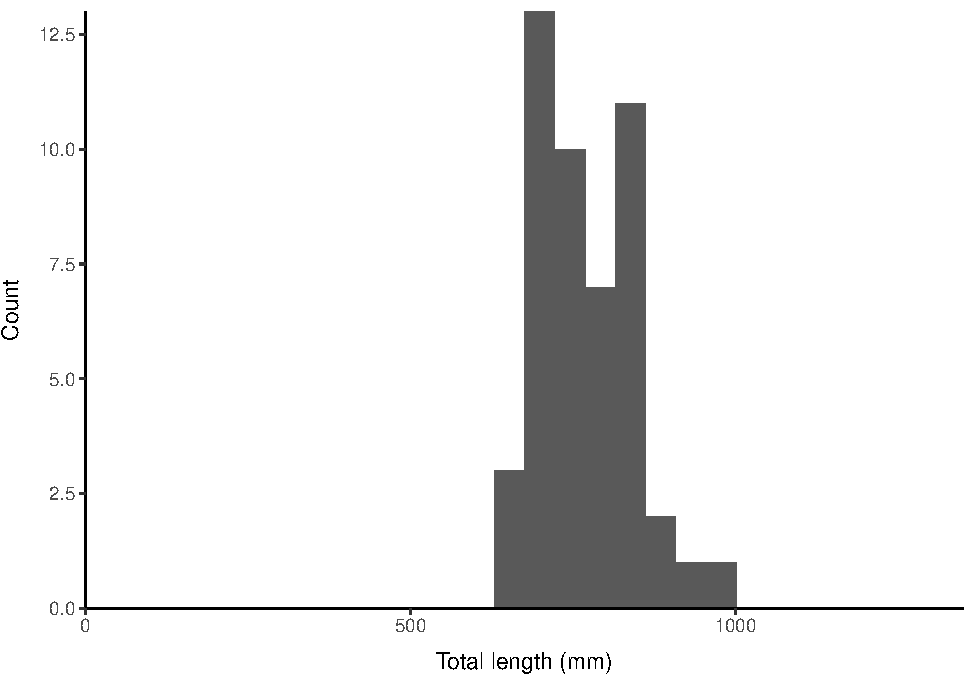
\includegraphics{worstr_files/figure-latex/unnamed-chunk-163-1.pdf}
Sure, looks totally normal to me? Wouldn't it be great if there were a statistical test for determining whether this sample is different from the normal? Great that you should ask.

\hypertarget{tests-of-normality-shapiro-wilk}{%
\paragraph{Tests of normality (Shapiro-Wilk)}\label{tests-of-normality-shapiro-wilk}}

The Shapiro-Wilk test is commonly used to test normality of a distribution as a check of assumptions. We can use this to test whether our data deviate from normal in the following manner:

\begin{Shaded}
\begin{Highlighting}[]
\KeywordTok{shapiro.test}\NormalTok{(age3_lengths)}
\end{Highlighting}
\end{Shaded}

\begin{verbatim}
## 
## 	Shapiro-Wilk normality test
## 
## data:  age3_lengths
## W = 0.95715, p-value = 0.07746
\end{verbatim}

First, note that the test statistic is the \texttt{W} statistic for this test.

Second, we have a p-value of \texttt{0.0774637}. \textbf{Oh, no}! Wait, what does that mean?

For this test, we actually don't want p \textless{} 0.05 if we are relying on assumptions of normality, so this is a ``good'' thing. But, it doesn't necessarily mean \texttt{age3\_lengths} is normally distributed. It just means that we can't tell if the sample we have collected is different from normal (we fail to reject the null but can't ``accept'' it). I guess that is good enough, but that p-value is awfully close to 0.05 for my taste.

So, are we up that proverbial tributary without a paddle, or can we salvage the mess and move on with life? Don't worry, there's a statistical test for that, too.

\hypertarget{wilcox-test}{%
\subsection{Wilcox test}\label{wilcox-test}}

You can think of the Wilcox test as a non-parametric analog of the t-test. In general, non-parametric tests tend to be slightly more ``conservative'' than the parametric alternatives because they require fewer assumptions. However, non-parametric tests can be useful where our data are not normal, or we don't feel we have sufficient data to know (hmm\ldots maybe don't conduct any tests, in that case!).

Here, we are checking for shifts in the median (not the mean) of one or more samples.

Why is this? The mean of a non-normal distribution is not always a useful descriptor of the probability mass under a distribution (it still describes `central tendency' but does not necessarily describe the place where `most of the data are'). But, the median always (as in always, always, always) describes central tendency of the data, so we can pretty much use it for describing any sample. This is because the median is defined as the ``middle'' value. That is, half of the data should fall on either side of the median if you lined up all of your data on the equator (wrong metaphor?).

\ldots back to the Wilcox test.

\begin{Shaded}
\begin{Highlighting}[]
\CommentTok{# First, do this and have a quick read:}
\NormalTok{  ?wilcox.test}
\end{Highlighting}
\end{Shaded}

Now we can actually run a test to see if the median length of age-3 fish is statistically different from the median value of length in the sample.

\begin{Shaded}
\begin{Highlighting}[]
    \KeywordTok{wilcox.test}\NormalTok{(}
\NormalTok{      age3_lengths,}
      \DataTypeTok{mu =} \KeywordTok{median}\NormalTok{(grasscarp}\OperatorTok{$}\NormalTok{Length),}
      \DataTypeTok{alternative =} \StringTok{'less'}\NormalTok{,    }\CommentTok{# Note different alternative here!}
      \DataTypeTok{exact =} \OtherTok{FALSE}            \CommentTok{# Not much data, so not exact}
\NormalTok{    )}
\end{Highlighting}
\end{Shaded}

\begin{verbatim}
## 
## 	Wilcoxon signed rank test with continuity correction
## 
## data:  age3_lengths
## V = 0, p-value = 8.414e-10
## alternative hypothesis: true location is less than 1007
\end{verbatim}

Interpretting the results is essentially the same as for the t-test, but without the degrees of freedom, so we won't belabor this. Importantly, the test, being robust to any distributional assumptions, should also (and does) tell us that the length of age-3 fish is significantly shorter than the population mean (or median- whichever you used).

\hypertarget{two-sample-tests}{%
\section{Two-sample tests}\label{two-sample-tests}}

Okay, with that out of the way, now we can get on to some tests that might be a little more meaningful to most people. We can use \textbf{two-sample} tests to whether two groups differ in some metric of interest. This lends itself naturally to use in controlled experiments that we conduct in laboratories, for example.

\hypertarget{the-two-sample-t-test}{%
\subsection{The two-sample t-test}\label{the-two-sample-t-test}}

If you have been exposed to only one statistical test already it is probably the two-sample t-test. This is a test that is used to test for differences in some continuous variable between two groups. The test statistic itself is pretty trivial to calculate. You can find a video of that \href{https://www.khanacademy.org/math/ap-statistics/two-sample-inference/two-sample-t-test-means/v/two-sample-t-test-for-difference-of-means}{here}. \textbf{Seriously, if you have never done a t-test, watch the 6-minute video now}. Otherwise, you may not understand what follows. I am not going to go into the math here because this is The Worst Stats Text eveR. The video will also help you understand how ANOVA and other tests work later. Understanding how these tests work will give you phenomenal cosmic powers when it comes to analyzing biological data. If you email asking me how a t-test works, I am going to send you this video.

Let's keep working with the \texttt{grasscarp} data for now for the sake of consistency. But, now we want to know if there is a difference in mean length of fish depending on whether their population density is high or low. To look at this, we'll need to make some groups in our \texttt{grasscarp} data that correspond to years of high and low density.

You can compare fish density between years quickly using the summary pipeline demonstrated in \protect\hyperlink{Chapter3}{Chapter 3}

\begin{Shaded}
\begin{Highlighting}[]
\NormalTok{grasscarp }\OperatorTok
\StringTok{  }\KeywordTok{group_by}\NormalTok{(Year) }\OperatorTok
\StringTok{  }\KeywordTok{summarize}\NormalTok{(}\DataTypeTok{dens =} \KeywordTok{unique}\NormalTok{(nha))}
\end{Highlighting}
\end{Shaded}

\begin{verbatim}
## # A tibble: 5 x 2
##    Year  dens
##   <int> <int>
## 1  2006    21
## 2  2007    58
## 3  2009    44
## 4  2010    43
## 5  2017   127
\end{verbatim}

You can see that density was much higher in \texttt{2017} than in any of the preceding years. This is because hydrilla area was reduced by several hundred hectares (\texttt{ha}) between 2010 and 2014 (which was actually the reason we went out to collect more data in 2017). But, these are just means and we need to be able to account for the variability in these measurements to call it science.

So, let's build some groups based on high and low density years. First, we'll add a new categorical variable to \texttt{grasscarp} called ``\texttt{density}'', and we'll fill it all in with the word \texttt{"low"} because there is only one year when density was high.

\begin{Shaded}
\begin{Highlighting}[]
\NormalTok{grasscarp}\OperatorTok{$}\NormalTok{density <-}\StringTok{ "low"}
\end{Highlighting}
\end{Shaded}

Next, we'll change all of the observations for 2017 to \texttt{"high"} so we have low density and high density groupings in our \texttt{density} column. This way, we only have to change the variable for one year.

\begin{Shaded}
\begin{Highlighting}[]
\NormalTok{grasscarp}\OperatorTok{$}\NormalTok{density[grasscarp}\OperatorTok{$}\NormalTok{Year }\OperatorTok{==}\StringTok{ }\DecValTok{2017}\NormalTok{] <-}\StringTok{ "high"}
\end{Highlighting}
\end{Shaded}

Then, we'll subset the data to look at a single age so our comparisons are fair between years. I picked \texttt{Age\ ==\ 10} because 10 years is in the middle of the range of ages in the data set. You can try it with another age as long as there are enough data.

\begin{Shaded}
\begin{Highlighting}[]
\NormalTok{mid_carps <-}\StringTok{ }\NormalTok{grasscarp }\OperatorTok\StringTok{ }\KeywordTok{subset}\NormalTok{(Age }\OperatorTok{==}\StringTok{ }\DecValTok{10}\NormalTok{)}
\end{Highlighting}
\end{Shaded}

Now, we can conduct our two-sample t-test!

The syntax is pretty straightforward, and is similar to what we used above, except that now we have two groups so we will omit \texttt{mu} and specify the t-test as a formula with independent (x, \texttt{density}) and dependent (y, \texttt{Length}) variables. There is no pairing of our observations, so we specify \texttt{paired\ =\ FALSE}, and we tell R we don't want to assume that the variance of \texttt{Length} is equal between \texttt{density} groups.

\begin{Shaded}
\begin{Highlighting}[]
  \KeywordTok{t.test}\NormalTok{(Length }\OperatorTok{~}\StringTok{ }\NormalTok{density,}
         \DataTypeTok{data =}\NormalTok{ mid_carps,}
         \DataTypeTok{paired =} \OtherTok{FALSE}\NormalTok{,      }\CommentTok{# 2-sample test, not "paired"}
         \DataTypeTok{var.equal =} \OtherTok{FALSE}\NormalTok{,   }\CommentTok{# We make no variance assumption}
         \DataTypeTok{conf.level =} \FloatTok{0.95}    \CommentTok{# Alpha = 0.05}
\NormalTok{    )}
\end{Highlighting}
\end{Shaded}

\begin{verbatim}
## 
## 	Welch Two Sample t-test
## 
## data:  Length by density
## t = -3.2263, df = 11.133, p-value = 0.007952
## alternative hypothesis: true difference in means is not equal to 0
## 95 percent confidence interval:
##  -190.03710  -36.03433
## sample estimates:
## mean in group high  mean in group low 
##           987.7143          1100.7500
\end{verbatim}

The interpretation of the results is much the same as with the one-sample t-test, except that we are now testing the null hypothesis that there is no difference between groups.

We reject the null hypothesis, and we conclude that age-10 fish were significantly larger during periods of low population density than they were during years of high population density (\emph{t} = \texttt{-3.2262903}, df = \texttt{11.1326183}, \emph{p} \textless{} 0.05). Makes perfect sense!

\hypertarget{assumptions-1}{%
\subsubsection{Assumptions}\label{assumptions-1}}

Equal variance

Now that we are using two samples, we should be cognizant that this test assumes equal variances in the independent variable between our two groups. If our variances are not equal, then we need to account for that (R actually assumes that the variances are unequal by default).

Let's test to see if the variances were equal between age-10 fish in the \texttt{high} and \texttt{low} density groups. To do this, we will conduct an F-test on the ratio of the two variances. If the ratio of the variances is different than one, we reject the null that the variances are the same.

\begin{Shaded}
\begin{Highlighting}[]
\KeywordTok{var.test}\NormalTok{(Length}\OperatorTok{~}\NormalTok{density, mid_carps)}
\end{Highlighting}
\end{Shaded}

\begin{verbatim}
## 
## 	F test to compare two variances
## 
## data:  Length by density
## F = 0.72988, num df = 20, denom df = 7, p-value = 0.5423
## alternative hypothesis: true ratio of variances is not equal to 1
## 95 percent confidence interval:
##  0.1634026 2.1950440
## sample estimates:
## ratio of variances 
##           0.729877
\end{verbatim}

Wow, this is way to easy. I hope that you are beginning to understand the \textbf{GLORY OF R}. This test could be a real pain in other software programs, and may not even be an option in many.

Back on topic\ldots we fail to reject the null hypothesis that the variances were equal. In this case, we now feel validated in the use of a two-sample t-test regardless of what R uses as the default (yes, sarcasm intended).

\hypertarget{normality}{%
\paragraph{Normality}\label{normality}}

Yes, we are still worried about this one because of the reasons given in the previous section. We can check this the same way as before. End of section.

\hypertarget{two-sample-wilcox-test}{%
\subsection{Two-sample Wilcox test}\label{two-sample-wilcox-test}}

If we were in violation of normality, we would use the Wilcox test to test for differences in ranks. I will not go through the whole thing again here. As with the t-test, if you have not been exposed to doing a rank-sum test by hand you really should \href{https://www.youtube.com/watch?v=AM87jjnNt8U}{\textbf{watch a video of how to do it}}. It really is easy once you've seen it and the video demystify the test for you.

I will note that the syntax is very much the same to that of the t-test now. This will pretty much stay the same for the next 6 chapters. Thank R, not me.

\begin{Shaded}
\begin{Highlighting}[]
\KeywordTok{wilcox.test}\NormalTok{(Length}\OperatorTok{~}\NormalTok{density, mid_carps)}
\end{Highlighting}
\end{Shaded}

\begin{verbatim}
## 
## 	Wilcoxon rank sum test with continuity correction
## 
## data:  Length by density
## W = 26, p-value = 0.005015
## alternative hypothesis: true location shift is not equal to 0
\end{verbatim}

As expected, this test also shows that the two samples differ significantly.

\emph{Note: this is equivelent to the Mann-Whitney U-test you may have learned about elsewhere. Had these samples been paired, R would have defaulted to a signed-rank test, with which you may also be familiar.}

\hypertarget{presenting-your-results}{%
\subsection{Presenting your results}\label{presenting-your-results}}

While it is important to report the test statistics, df, etc., it can be just as meaningful to give the sample means (reported in the \texttt{t.test}) and show a graph. \textbf{Remember}: don't make shitty graphs. Be proud of your results and show your readers what they mean.

In this case, a boxplot or a violin plot would work great. We haven't looked at violin plots yet, so let's give them a whirl!

Violins are a lot like box plots except they give us a little better visual description of the shape of sampling distributions within groups. I added some \texttt{ggplot2} functions to control fill and color of the violins in the example below. You can check out \href{https://www.datanovia.com/en/blog/ggplot-colors-best-tricks-you-will-love/\#predefined-ggplot-color-palettes}{this blog post} for some other cool examples with other \texttt{ggplot} geometries. Play around with the plotting code above to change what you like. Remember, all of the customization achieved using the \texttt{theme()} function is the same across plot types.

Here is a quick, ugly violin plot with some basic options. Pretty easy to make, but also kind of makes you want to puke.

\begin{Shaded}
\begin{Highlighting}[]
\KeywordTok{ggplot}\NormalTok{(mid_carps, }\KeywordTok{aes}\NormalTok{(}\DataTypeTok{x =}\NormalTok{ density, }\DataTypeTok{y =}\NormalTok{ Length)) }\OperatorTok{+}\StringTok{ }
\StringTok{  }\KeywordTok{geom_violin}\NormalTok{(}\KeywordTok{aes}\NormalTok{(}\DataTypeTok{group =}\NormalTok{ density), }\DataTypeTok{trim =} \OtherTok{FALSE}\NormalTok{)}
\end{Highlighting}
\end{Shaded}

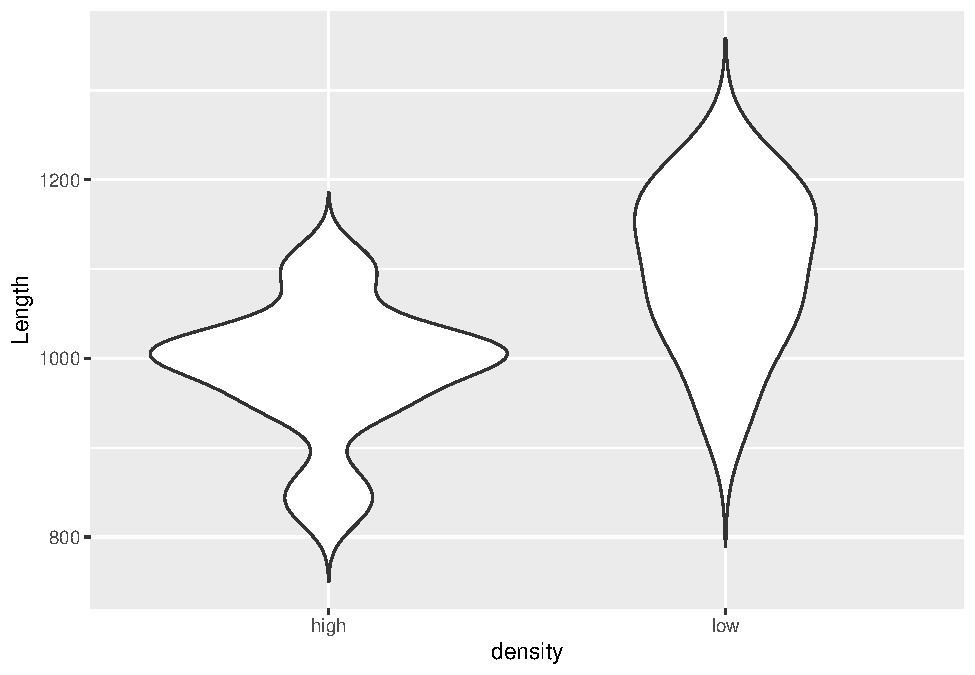
\includegraphics{worstr_files/figure-latex/unnamed-chunk-175-1.pdf}

Here is a much better plot. Not that much more difficult to make, and doesn't make you want to puke even if the code does a little bit.

\begin{Shaded}
\begin{Highlighting}[]
\NormalTok{mid_carps }\OperatorTok
\KeywordTok{ggplot}\NormalTok{(}\KeywordTok{aes}\NormalTok{(}\DataTypeTok{x =}\NormalTok{ density, }\DataTypeTok{y =}\NormalTok{ Length, }\DataTypeTok{fill =}\NormalTok{ density, }\DataTypeTok{color =}\NormalTok{ density)) }\OperatorTok{+}\StringTok{ }
\StringTok{  }\KeywordTok{geom_violin}\NormalTok{(}\KeywordTok{aes}\NormalTok{(}\DataTypeTok{group =}\NormalTok{ density), }\DataTypeTok{trim =} \OtherTok{FALSE}\NormalTok{, }\DataTypeTok{size =} \FloatTok{.75}\NormalTok{) }\OperatorTok{+}
\StringTok{  }\KeywordTok{scale_x_discrete}\NormalTok{(}\DataTypeTok{breaks=}\KeywordTok{c}\NormalTok{(}\StringTok{"high"}\NormalTok{, }\StringTok{"low"}\NormalTok{), }\DataTypeTok{labels =} \KeywordTok{c}\NormalTok{(}\StringTok{"High"}\NormalTok{, }\StringTok{"Low"}\NormalTok{)) }\OperatorTok{+}
\StringTok{  }\KeywordTok{scale_fill_grey}\NormalTok{(}\DataTypeTok{start =} \FloatTok{0.9}\NormalTok{, }\DataTypeTok{end =} \FloatTok{0.4}\NormalTok{) }\OperatorTok{+}
\StringTok{  }\KeywordTok{scale_color_grey}\NormalTok{(}\DataTypeTok{start =} \FloatTok{0.8}\NormalTok{, }\DataTypeTok{end =} \FloatTok{0.3}\NormalTok{) }\OperatorTok{+}
\StringTok{  }\KeywordTok{xlab}\NormalTok{(}\StringTok{"Density"}\NormalTok{) }\OperatorTok{+}
\StringTok{  }\KeywordTok{ylab}\NormalTok{(}\StringTok{"Total length (mm) at age 10"}\NormalTok{) }\OperatorTok{+}
\StringTok{  }\KeywordTok{labs}\NormalTok{(}\DataTypeTok{fill =} \StringTok{"Density"}\NormalTok{, }\DataTypeTok{color =} \StringTok{"Density"}\NormalTok{) }\OperatorTok{+}
\StringTok{  }\KeywordTok{theme_bw}\NormalTok{() }\OperatorTok{+}
\StringTok{  }\KeywordTok{theme}\NormalTok{(}
    \DataTypeTok{axis.title.x =} \KeywordTok{element_text}\NormalTok{(}\DataTypeTok{vjust =} \DecValTok{-1}\NormalTok{),}
    \DataTypeTok{axis.title.y =} \KeywordTok{element_text}\NormalTok{(}\DataTypeTok{vjust =} \DecValTok{3}\NormalTok{),}
    \DataTypeTok{panel.grid =} \KeywordTok{element_blank}\NormalTok{()}
\NormalTok{  )}
\end{Highlighting}
\end{Shaded}

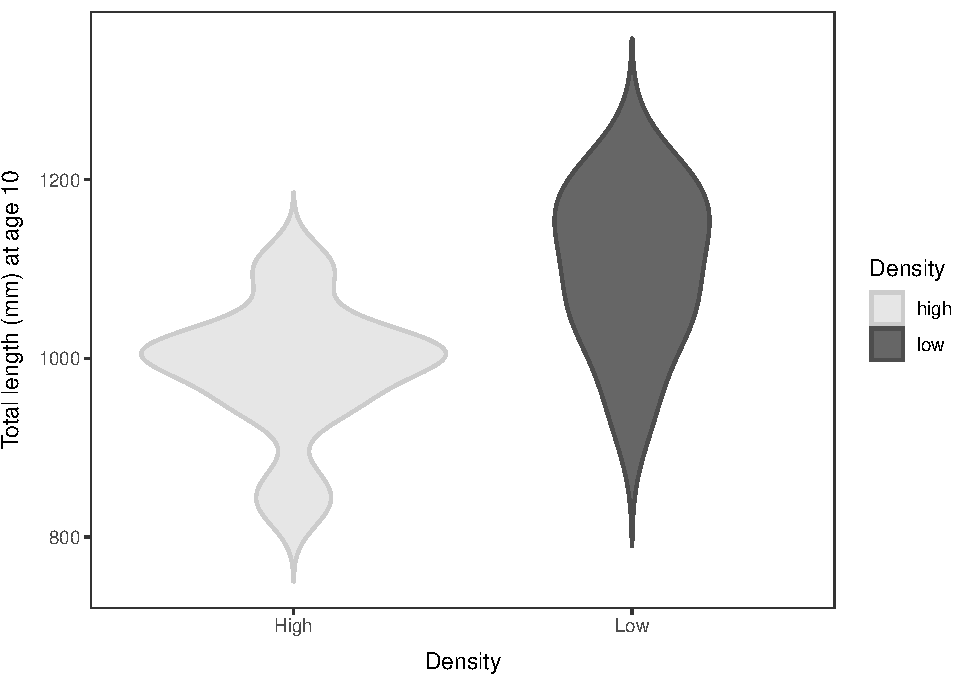
\includegraphics{worstr_files/figure-latex/unnamed-chunk-176-1.pdf}

There, isn't that fancy? I think that gives you a much more detailed understanding of how \texttt{Length} varies between \texttt{high} and \texttt{low} population density than a simple p-value. But, maybe its just me\ldots{}

\hypertarget{frequency-analysis}{%
\section{Frequency analysis}\label{frequency-analysis}}

Now, what if we didn't collect very good data, or we binned our data into low-resolution categories for the sake of ease in our study design? Often, and for a variety of reasons other than crappy data collection, we want to compare frequencies of events between two (or more) groups. We may even design studies specifically to test these kinds of hypotheses when we think about rates, for example. This is very common in studies of population genetics {[}definitely citations available for that one - go Google them{]}

The simplest way to test for differences in the frequency of a categorical response between two groups is (some would argue) the \(\chi^2\) test. The \(\chi^2\) is another one of those that you should really work out by hand because it is used in a variety of settings ``under the hood'' of more complex routines. Here is your token \href{https://www.youtube.com/watch?v=V4SRgabFbz0}{video link showing and example}. Watch it. Please.

\hypertarget{worked-example}{%
\subsection{Worked example}\label{worked-example}}

Let's say we want to know if the number of grass carp in a given age group (say age 10) varies between years. These fish are sterile hybrids, so we would expect that the number of fish in each age would change drastically with increasing time since the year of initial stocking (1995).

First, make a table showing the number of fish in each \texttt{Age} by \texttt{Year} with the \texttt{grasscarp} data.

\begin{Shaded}
\begin{Highlighting}[]
\NormalTok{agexyear <-}\StringTok{ }\KeywordTok{with}\NormalTok{(grasscarp, }\KeywordTok{table}\NormalTok{(Age, Year))}

\KeywordTok{print}\NormalTok{(agexyear)}
\end{Highlighting}
\end{Shaded}

\begin{verbatim}
##     Year
## Age  2006 2007 2009 2010 2017
##   1     0    0    0    2    0
##   2     6    7    7    8    0
##   3    11   10   10   14    3
##   4     4    3    6    3    3
##   5     0    1    3    2   10
##   6     0    1    2    1   12
##   7     0    0    1    3   11
##   8     0    1    1    2   12
##   9     1    0    1    3   21
##   10    4    1    1    2   21
##   11    4    9    0    6   15
##   12    3   15    2    3   18
##   13    0    1    4    3    7
##   14    0    0   11    8    6
##   15    0    0    2   12   12
##   16    0    0    0    2   10
##   17    0    0    0    0    8
##   18    0    0    0    0    9
##   19    0    0    0    0   12
##   20    0    0    0    0   12
##   21    0    0    0    0    5
##   22    0    0    0    0    3
##   23    0    0    0    0    2
\end{verbatim}

Basically what we are going to do is analyze the proportion of total fish in each column

You should see some pretty obvious patterns here. We have a couple of things to think about now. First, this is the kind of question you don't need statistics for. Second, we have a whole bunch of empty groups, and these are not random with respect to year. Some of these come from ages that were not yet available in years 2006 - 2010 and some from patterns in fish stocking. The large number of empty pairings and the fact that most age classes had fewer than five fish in any year prior to 2017 means we should probably break the data down a little further. This stinks because we lose resolution, but that is the cost.

For the sake of demonstration, let's summarize the data by \texttt{high} and \texttt{low} density again and we'll look at the number of fish collected in each age class during high and low density years.

\begin{Shaded}
\begin{Highlighting}[]
\NormalTok{freqs <-}\StringTok{ }\NormalTok{grasscarp }\OperatorTok\StringTok{ }\CommentTok{# Pass grass carp data frame to group_by()}
\StringTok{    }\KeywordTok{filter}\NormalTok{(Age }\OperatorTok\StringTok{ }\KeywordTok{c}\NormalTok{(}\DecValTok{10}\OperatorTok{:}\DecValTok{15}\NormalTok{)) }\CommentTok{# Select only shared age range}

\KeywordTok{head}\NormalTok{(freqs)}
\end{Highlighting}
\end{Shaded}

\begin{verbatim}
##   Year Length Weight_kg Age cohort n_stocked     n acre   ha nha     kg kg_ha
## 1 2006   1262    23.154  12   1994      7000 25128 2957 1203  21 129929   108
## 2 2006   1138    23.923  10   1996      7000 25128 2957 1203  21 129929   108
## 3 2006   1187    18.614  10   1996      7000 25128 2957 1203  21 129929   108
## 4 2006   1207    19.522  12   1994      7000 25128 2957 1203  21 129929   108
## 5 2006   1086    21.285  10   1996      7000 25128 2957 1203  21 129929   108
## 6 2006   1095    18.160  12   1994      7000 25128 2957 1203  21 129929   108
##   density
## 1     low
## 2     low
## 3     low
## 4     low
## 5     low
## 6     low
\end{verbatim}

We will test the null hypothesis that there is no difference in the number of age-10 fish between high and low densities.

\begin{Shaded}
\begin{Highlighting}[]
\CommentTok{# Run the test}
\NormalTok{chi_test <-}\StringTok{ }\KeywordTok{with}\NormalTok{(freqs, }\KeywordTok{chisq.test}\NormalTok{(}\DataTypeTok{x =}\NormalTok{ density, }\DataTypeTok{y =}\NormalTok{ Age))}

\CommentTok{# Have a look}
\KeywordTok{print}\NormalTok{(chi_test)}
\end{Highlighting}
\end{Shaded}

\begin{verbatim}
## 
## 	Pearson's Chi-squared test
## 
## data:  density and Age
## X-squared = 13.107, df = 5, p-value = 0.0224
\end{verbatim}

And, bam! We see that there is a difference in the frequency of fish collected in each age class in high and low density years. Shocker.

Data visualization techniques for contingency table analyses like this seem to have generally lagged behind theory in terms of wide-spread implementation. There is a base R \texttt{mosaicplot} that plots relative freqencies. You can interpret the width of the bars as the proportion of total observations in each age class. Likewise, the height of the vertical segnmens corresponds to proportion of \texttt{high} or \texttt{low} \texttt{density} observations in each \texttt{Age}.

\begin{Shaded}
\begin{Highlighting}[]
\KeywordTok{mosaicplot}\NormalTok{(Age }\OperatorTok{~}\StringTok{ }\NormalTok{density, }\DataTypeTok{data =}\NormalTok{ freqs)}
\end{Highlighting}
\end{Shaded}

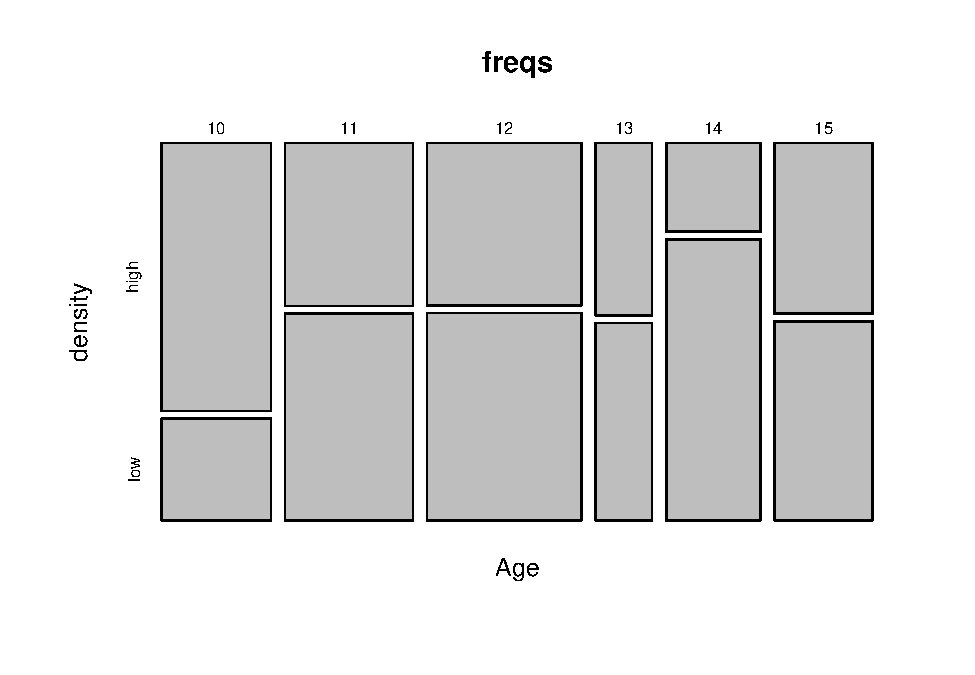
\includegraphics{worstr_files/figure-latex/unnamed-chunk-180-1.pdf}

The need for improved graphical representation for these data types is recognized. There have been recent efforts to extend the philosophies used \texttt{ggplot()} to contingency analysis by r developers (see Wickham and Hofmann 2011\textless\textgreater). It was even the topic of a recent master's thesis (see Grant 2017). But as far as I know the ideas from these works have not been integrated into \texttt{ggplot2} or the \texttt{tidyverse} yet. Sorry about the citations. I don't know what I was thinking. This is supposed to be the Worst Stats Text eveR.

\hypertarget{next6}{%
\section{Next steps}\label{next6}}

In this chapter, we introduced inferential statistics and walked through examples of a few simple statistical tests for comparing samples to one another using two-sample tests, or to a single value using a one-sample test. In \protect\hyperlink{Chapter7}{Chapter 7} we will continue to build on these tools as we press on to linear models and the rest of statistics.

  \bibliography{book.bib,packages.bib}

\end{document}
